\chapter{Results}
\label{chap:results}
This chapter assesses the computational implementation accomplished by the author. The aim is to determine if the programming and computational implementation of the model is correct. The implementation in syn3D and NX Flow are validated on the following cases:
\begin{itemize}
    \item Flat plate (syn3D \& NX Flow)
    \item Two-dimensional bump (syn3D)
    \item Three-dimensional bump (syn3D)
    \item NACA 0012 (NX Flow)
    \item RAE 2822 (syn3D \& NX Flow)
    \item High-lift configuration 30P30N (syn3D)
\end{itemize}
The first four cases are taken from the Turbulence Modeling Resource (TMR)~\cite{tmr}, which provides a set of grids as well as results from established CFD codes, namely CFL3D and FUN3D, which are developed at NASA. 

It should be noted that the difference in results using either wall distance methods (brute force and Poisson) was negligible and a comparison between the results obtained with the two methods is not shown.
\section{Flat plate}
The turbulent flow over a flat plate is investigated. All grids and results are available in~\cite{tmr} under the name: ``2D Zero pressure gradient flat plate''. The problem domain and flow conditions are shown in~\Cref{fig:flat}. NX Flow does not offer far-field BCs and uses an inlet BC on the leftmost face and openings on the top and rightmost face. Moreover, the problem was run with a fixed density in NX Flow so as to reduce computational cost, since this is essentially an incompressible case.

The Turbulence Modeling Resource provides five grids, each finer than the next, in order to compare so-called mesh independent results and to perform a grid study. The goal of a grid study is to establish that the obtained results will not vary significantly by further refining the mesh, and thus that the obtained results are as accurate as possible.
\begin{figure}
    \centering
    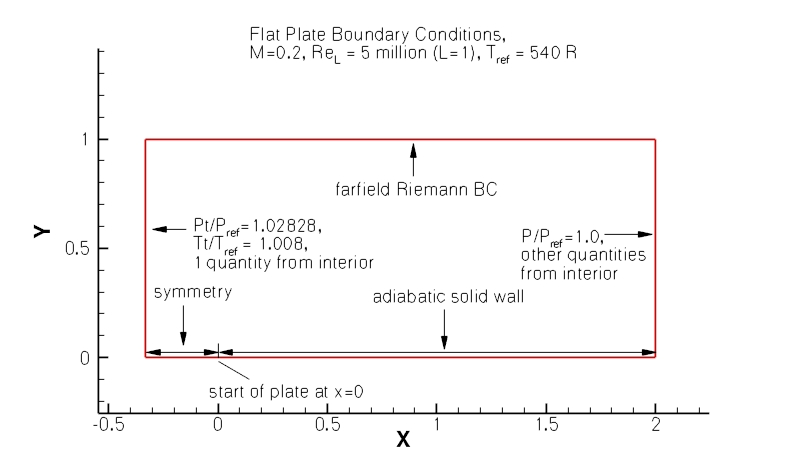
\includegraphics[width=0.7\textwidth]{figs/flat/flatplate.png}
    \caption{Turbulent flat plate case~\cite{tmr}.}
    \label{fig:flat}
\end{figure}

The skin friction coefficient $C_f$ at $x = 0.97$ and drag coefficient $C_D$ are compared to CFL3D, a cell-centered finite volume code developed by NASA, in~\Cref{tab:flat}. These coefficients are calculated as:
\begin{align*}
    C_f = \frac{2\tau_w}{\rho_\infty U_\infty^2}\\
    C_D = \frac{2D}{\rho_\infty U_\infty^2 A},
\end{align*}
where $D$ is the drag force and $A$ the reference area. For this case, the reference area is the length of the plate times its width, i.e. the length of the mesh in the $z$ direction. \Cref{tab:flat} tabulates the skin friction coefficient and drag coefficient values.
All values are within 2\% of each other. Reasons for discrepancies are given below.
\begin{table}
\centering
\caption{Flat Plate (syn3D \& NX Flow): Comparison of force coefficients on the finest grid.}
\label{tab:flat}
\begin{tabular}{@{}lcc@{}}
    \toprule
    Solver & $C_D$ & $C_f$ at $x=0.97$ \\
    \midrule
    CFL3D & 0.00286 & 0.00270 \\
    NX Flow & 0.00288 & 0.00272 \\
    syn3D & 0.00280 & 0.00269\\
    \bottomrule
\end{tabular}
\end{table}
\Cref{fig:synflatcnvstudy} shows the residual convergence of the density residual and turbulence residual for all grids with syn3D. \Cref{fig:nxflatcnvstudy} shows the residual of all equations for all grids with NX Flow. As expected, the coarser grids show faster convergence than the finer ones -- this phenomenon is detailed in~\cite{blazek2015computational}. While the residual was never driven down to machine precision, differences in the obtained solution field were found to be marginal by further reducing the residual.

\Cref{tab:flatcpu} compares the number of iterations and CPU time between syn3D and NX Flow for the medium grid, which demonstrates the advantages of an implicit solver over an explicit solver: around two thousand times more iterations are taken by syn3D. On the other hand, explicit iterations are much less computationally expensive and require less storage. It should also be noted that NX Flow does not solve the conservation of energy equation for this particular case, since it uses a fixed density. Moreover, multigrid was not used with syn3D for this case, which significantly accelerates convergence in most cases.
\begin{table}
\caption{Flat Plate (syn3D \& NX Flow): Convergence metrics on the medium grid.}
\label{tab:flatcpu}
\begin{tabular}{@{}l ccccc@{}}
\toprule
Solver & Processors & Iterations & Time taken & Time per iteration & Residual reduction \\
       &            &            & (min)      & (sec)              &                    \\
\midrule
% NX Flow (4 cores) & 205 & 34 & $\approx$ 10 & $10^{-10}$ \\
% syn3D (8 cores) & 400000 & 156 & $\approx$ 0.023 & $10^{-8}$
NX Flow & 4 & 205 & 34 & $\approx$ 10 & $10^{-10}$ \\
syn3D & 8 & 400000 & 156 & $\approx$ 0.023 & $10^{-8}$
\\
\bottomrule
\end{tabular}
\end{table}

\begin{figure}[ht!]
\centering
\begin{subfigure}{.45\textwidth}
  \centering
  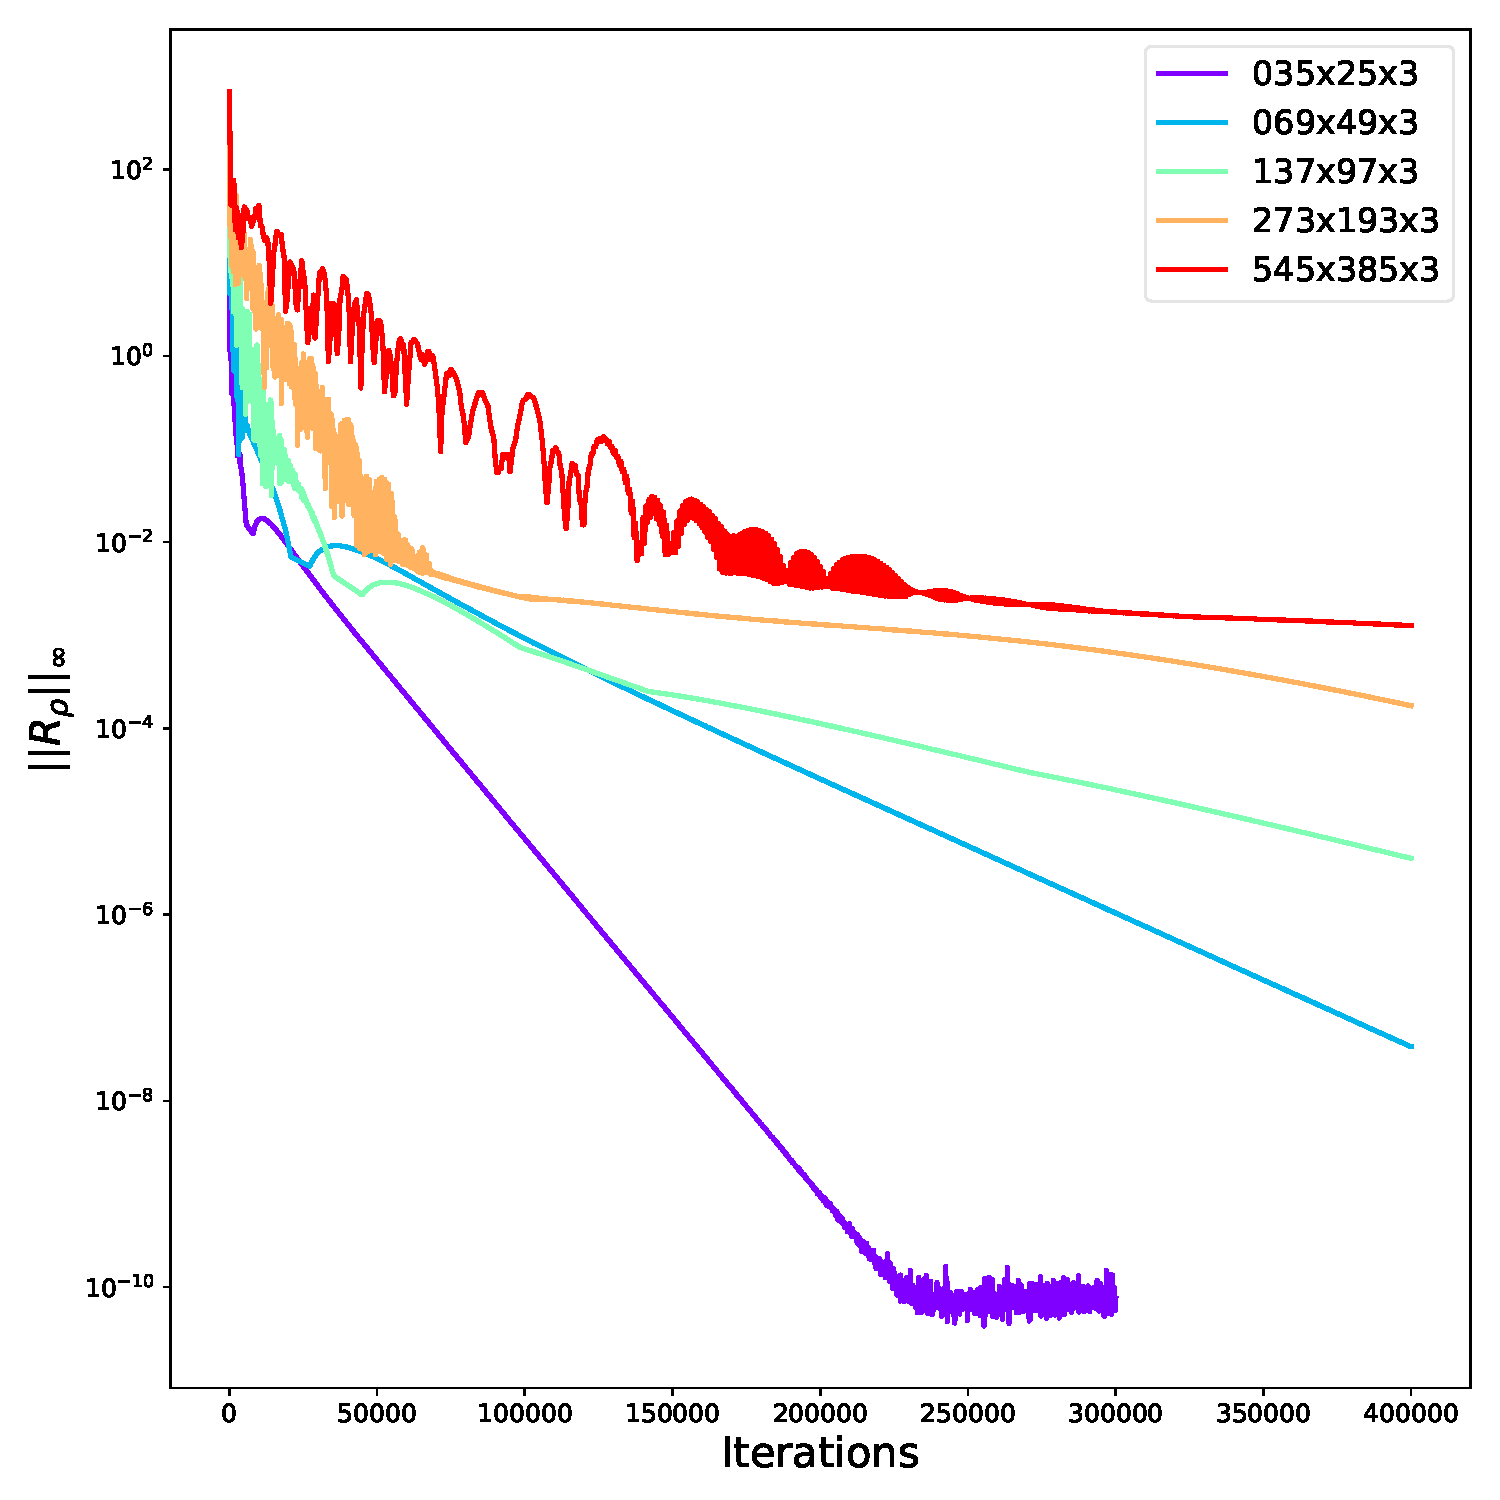
\includegraphics[width=1.0\textwidth]{figs/flat/gov_convergence_gridstudy.pdf}
  \caption{Maximum density residual.}
\end{subfigure}%
\begin{subfigure}{.45\textwidth}
    \centering
    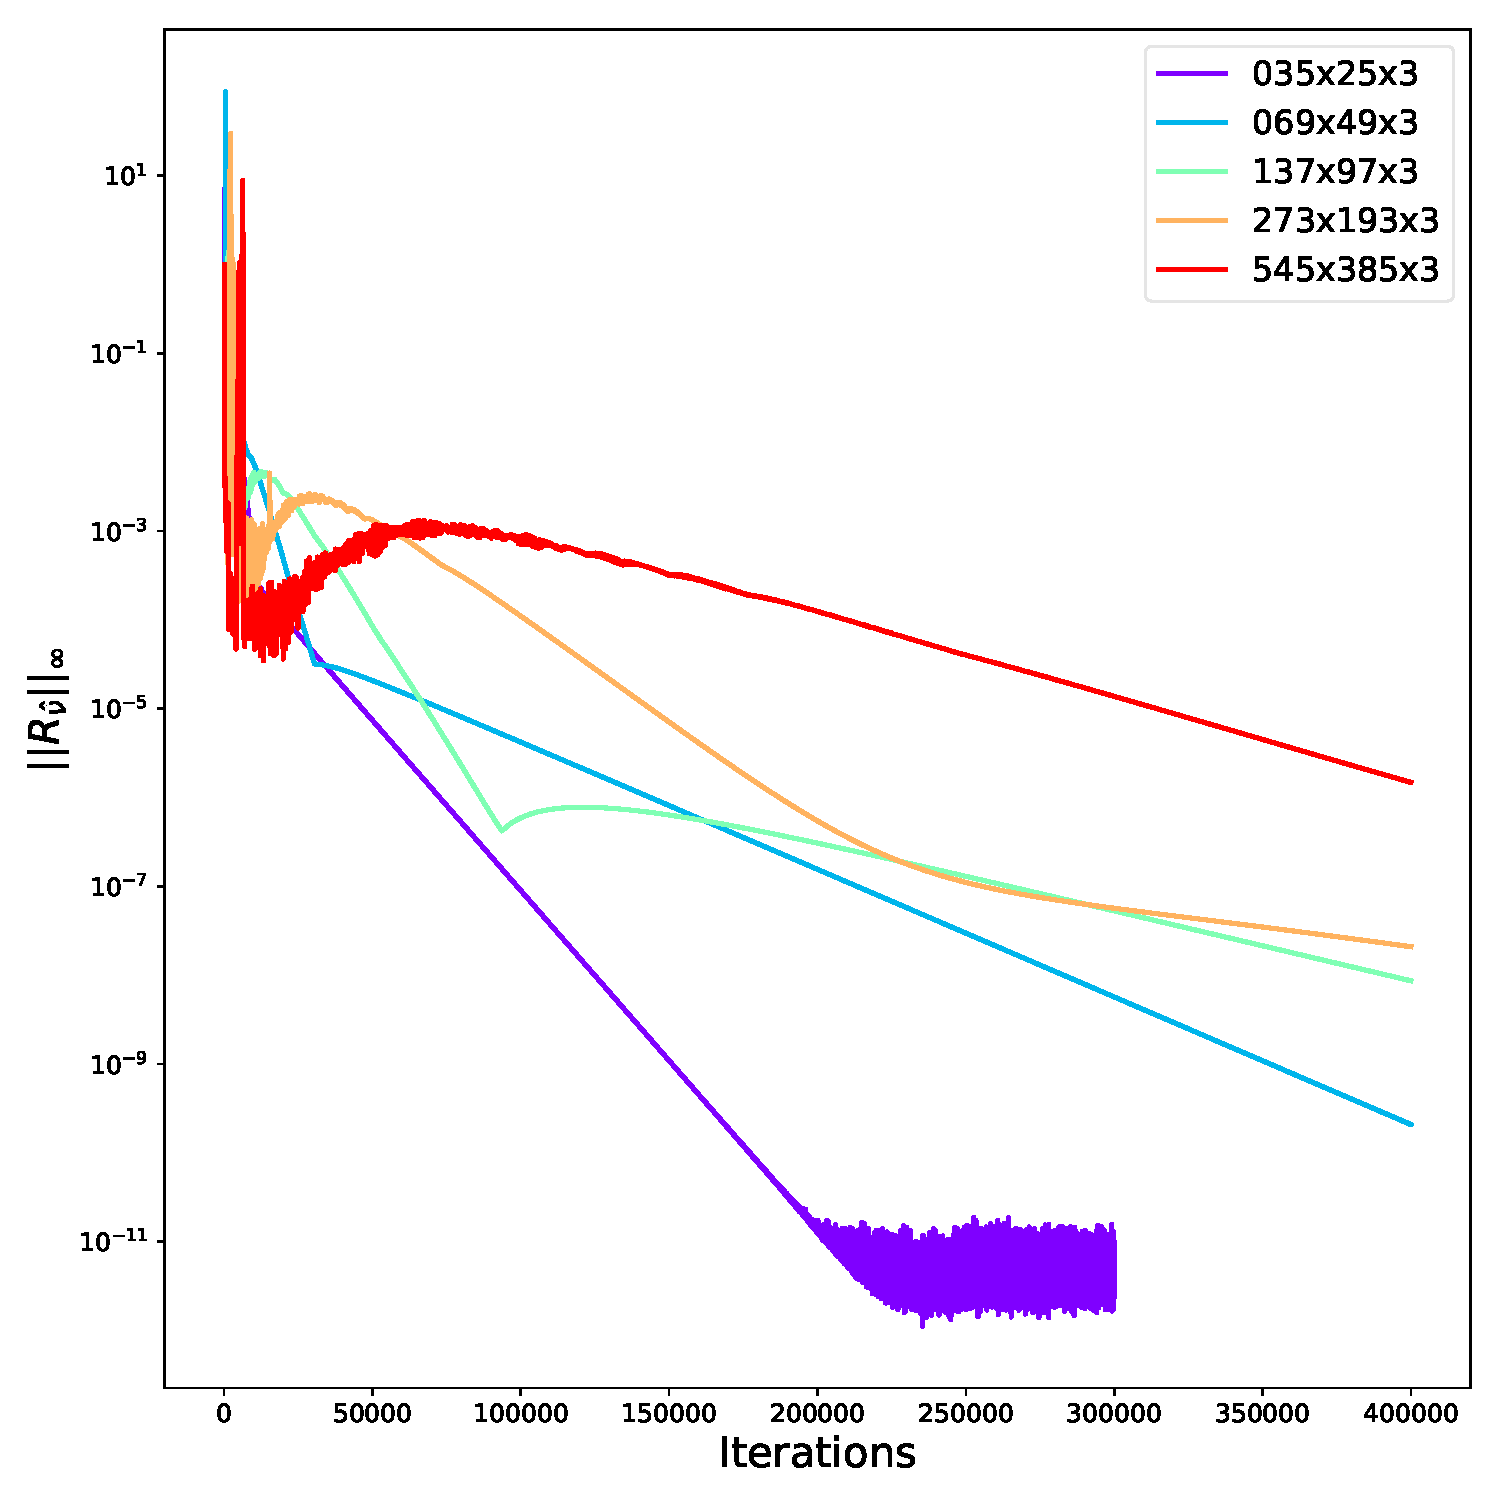
\includegraphics[width=1.0\textwidth]{figs/flat/SA_convergence_gridstudy.pdf}
    \caption{Maximum turbulence variable residual.}
\end{subfigure}
\caption{Flat Plate (syn3D): Convergence of flow and turbulence variables on various grid sizes.}
\label{fig:synflatcnvstudy}
\end{figure}
\begin{figure}[ht!]
    \centering
    \begin{subfigure}{0.48\textwidth}
        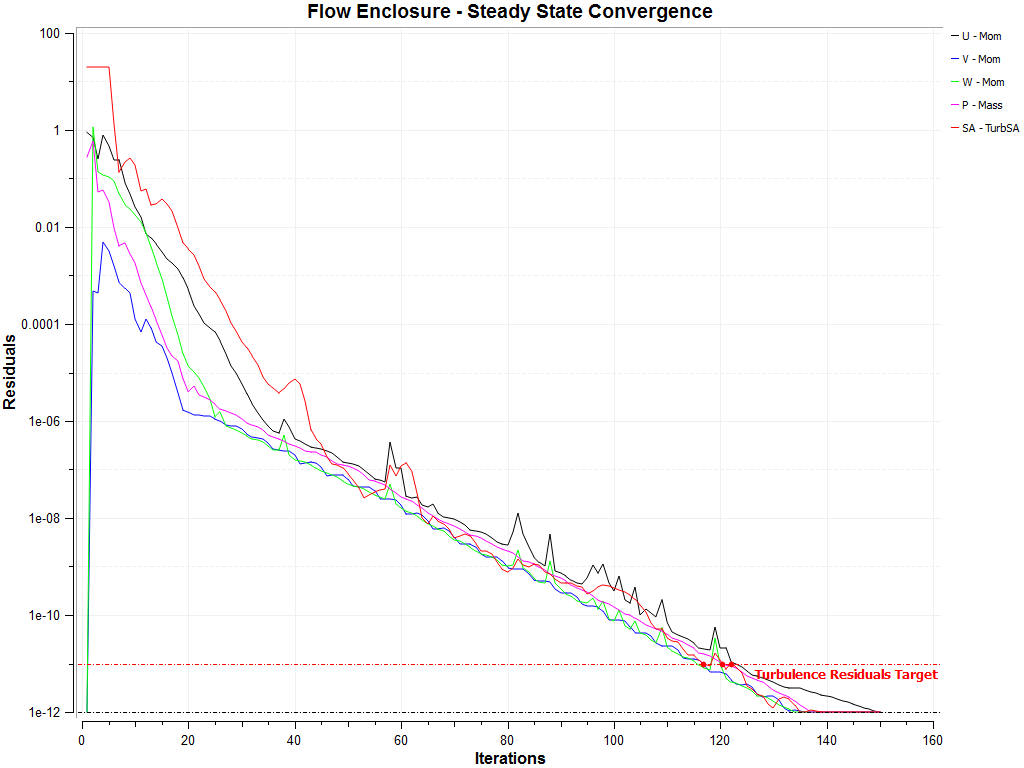
\includegraphics[width=\textwidth]{./figs/flatnx/35x25_conv.png}
        \caption{35x25}
    \end{subfigure}
    \hfill
    \begin{subfigure}{0.48\textwidth}
        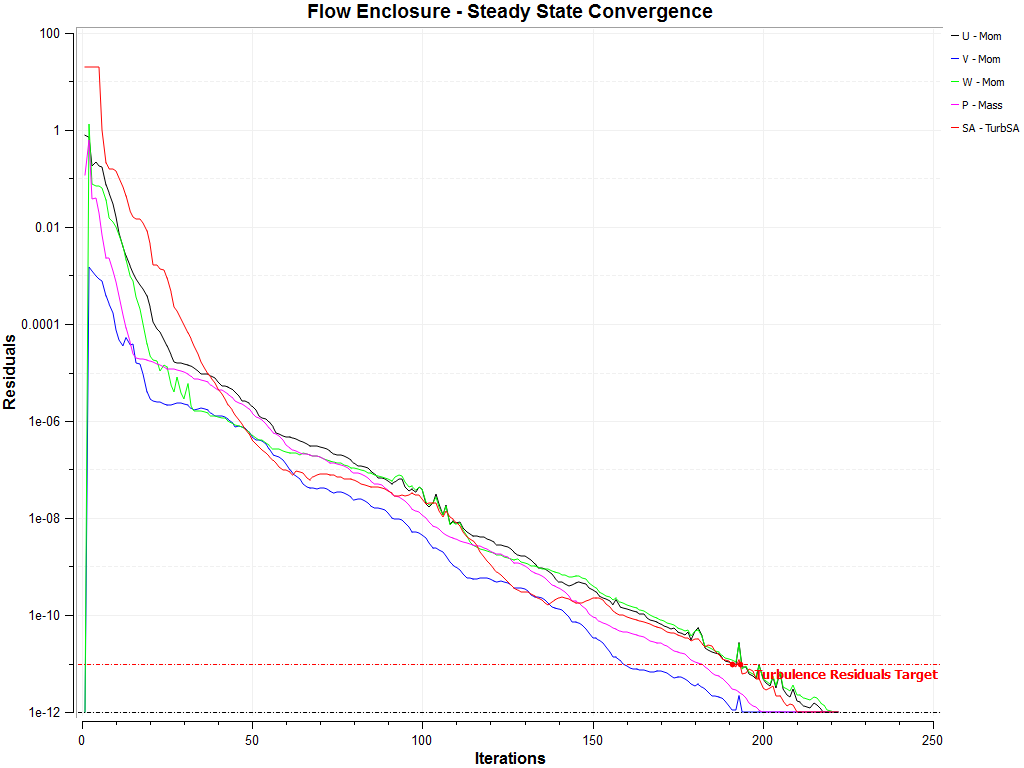
\includegraphics[width=\textwidth]{./figs/flatnx/69x49_conv.png}
        \caption{69x49}
    \end{subfigure}
    \\
    \begin{subfigure}{0.48\textwidth}
        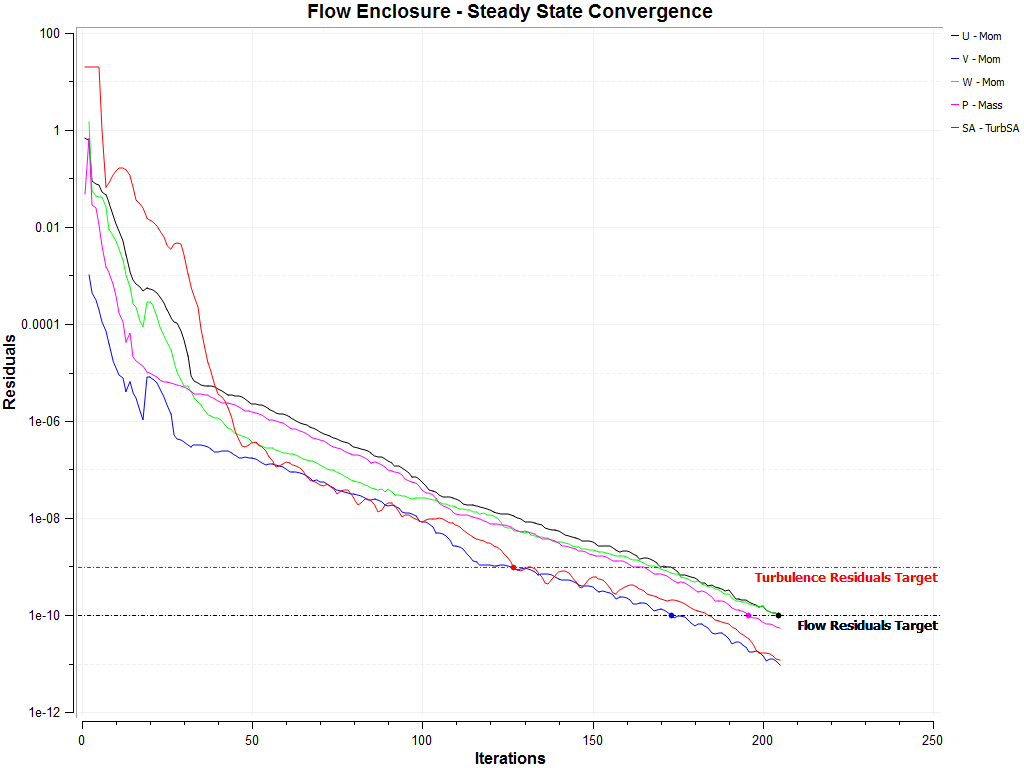
\includegraphics[width=\textwidth]{./figs/flatnx/137x97_conv.png}
        \caption{137x97}
    \end{subfigure}
    \hfill
    \begin{subfigure}{0.48\textwidth}
        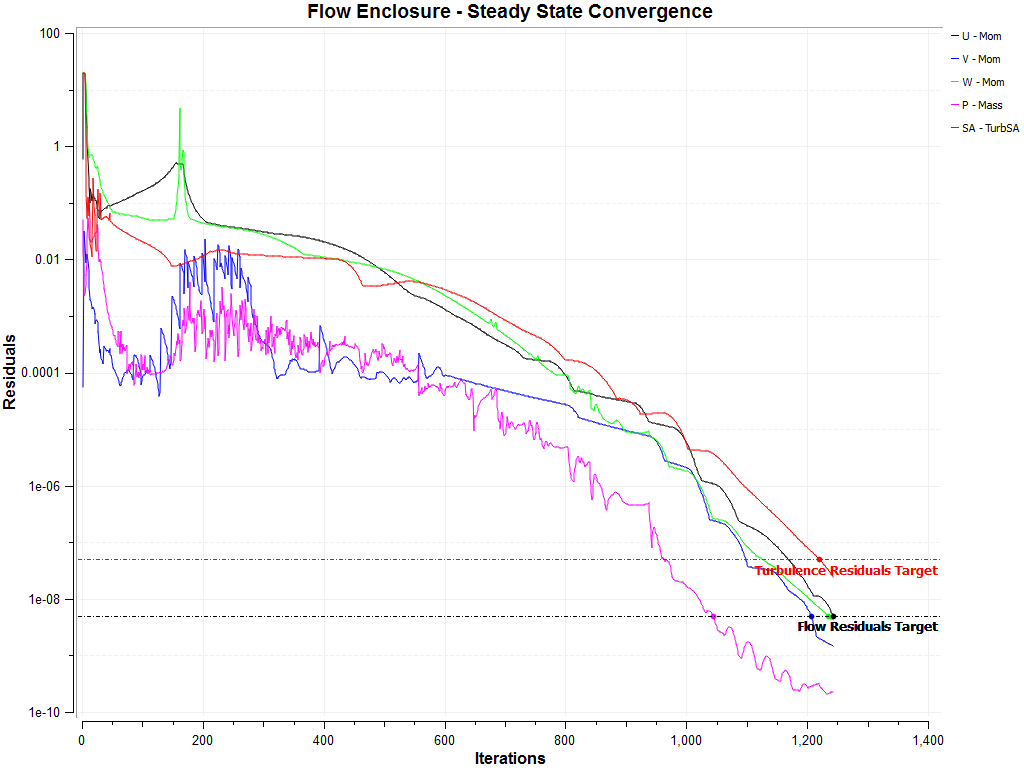
\includegraphics[width=\textwidth]{./figs/flatnx/273x193_conv.png}
        \caption{273x193}
    \end{subfigure}
    \\
    \begin{subfigure}{0.48\textwidth}
        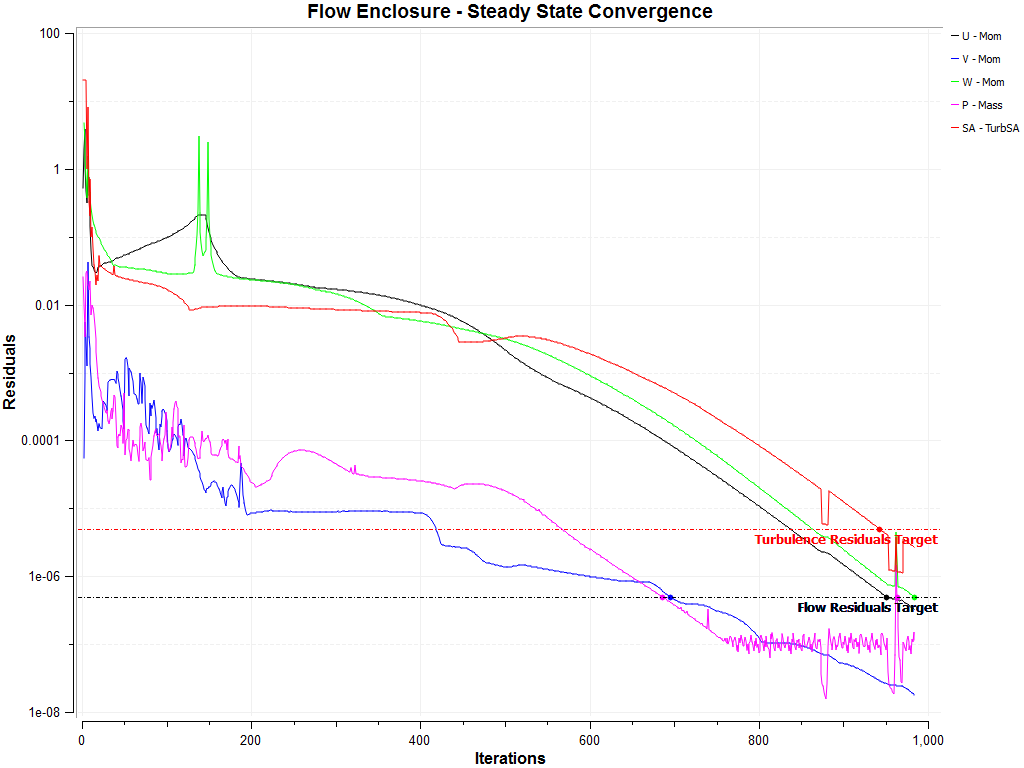
\includegraphics[width=\textwidth]{./figs/flatnx/545x385_conv.png}
        \caption{545x385}
    \end{subfigure}
    \caption{Flat Plate (NX Flow): Convergence of residuals on various grid sizes.}
    \label{fig:nxflatcnvstudy}
\end{figure}

Several plots have been generated to compare the results between all solvers. Unless otherwise noted, all results were obtained with the finest grid. \Cref{fig:flatcf} compares the skin friction along the plate, which is maximal at the leading edge and then gradually decreases. NX Flow and syn3D display slight over-prediction and under-prediction respectively. The skin friction coefficient is a measure of the velocity gradient at the wall.

\Cref{fig:flatmutcontour} shows contour plots of the dimensionless eddy viscosity $\frac{\mu_t}{\mu_{\infty}}$ and \Cref{fig:flatmu} shows line plots of the dimensionless eddy viscosity. As expected, the eddy viscosity increases gradually as the wall distance increases, as turbulence effects are more significant in the log-law region, and then diminishes as it reaches the far-field region. This is in accordance with the law of the wall, which states that turbulent stresses are minimal in the viscous sublayer and maximal in the log-law layer. Moreover, the eddy viscosity, initially close to zero, increases with $x$ due to production near the wall as well as advection.

\Cref{fig:flatu,fig:flatupyp} show profiles of the dimensionless velocity $u/u_\infty$ and $u^+$ respectively. The velocity profile shows a sharp gradient near the wall, typical of turbulent flows. Moreover, the height of the boundary layer, the region where velocity is reduced as compared to the far-field, grows with increasing $x$. It can also be seen that the $u^+$ profile agrees with the theory: $u^+$ follows the $u^+=y^+$ curve in the viscous sublayer and the log-law curve in the log-law region.

Overall, there is excellent agreement between NX Flow and CFL3D and some level of discrepancy between syn3D and CFL3D. The source of discrepancy is easily seen in~\Cref{fig:flatmutmax}: the eddy viscosity jumps abruptly right at the leading edge for syn3D but not for the other two. It should be noted that the spike occurs at the interface between block boundaries, which could be the cause of this phenomenon. These blocks thus have different boundary conditions at their $y=0$ face. Moreover, the jump does not occur if the domain only includes the plate, i.e. starts at $x=0$.
% The cause of this jump was investigated by the author as well as others working on the code, but a definite answer was unfortunately not found.
\begin{figure}[ht!]
\centering
	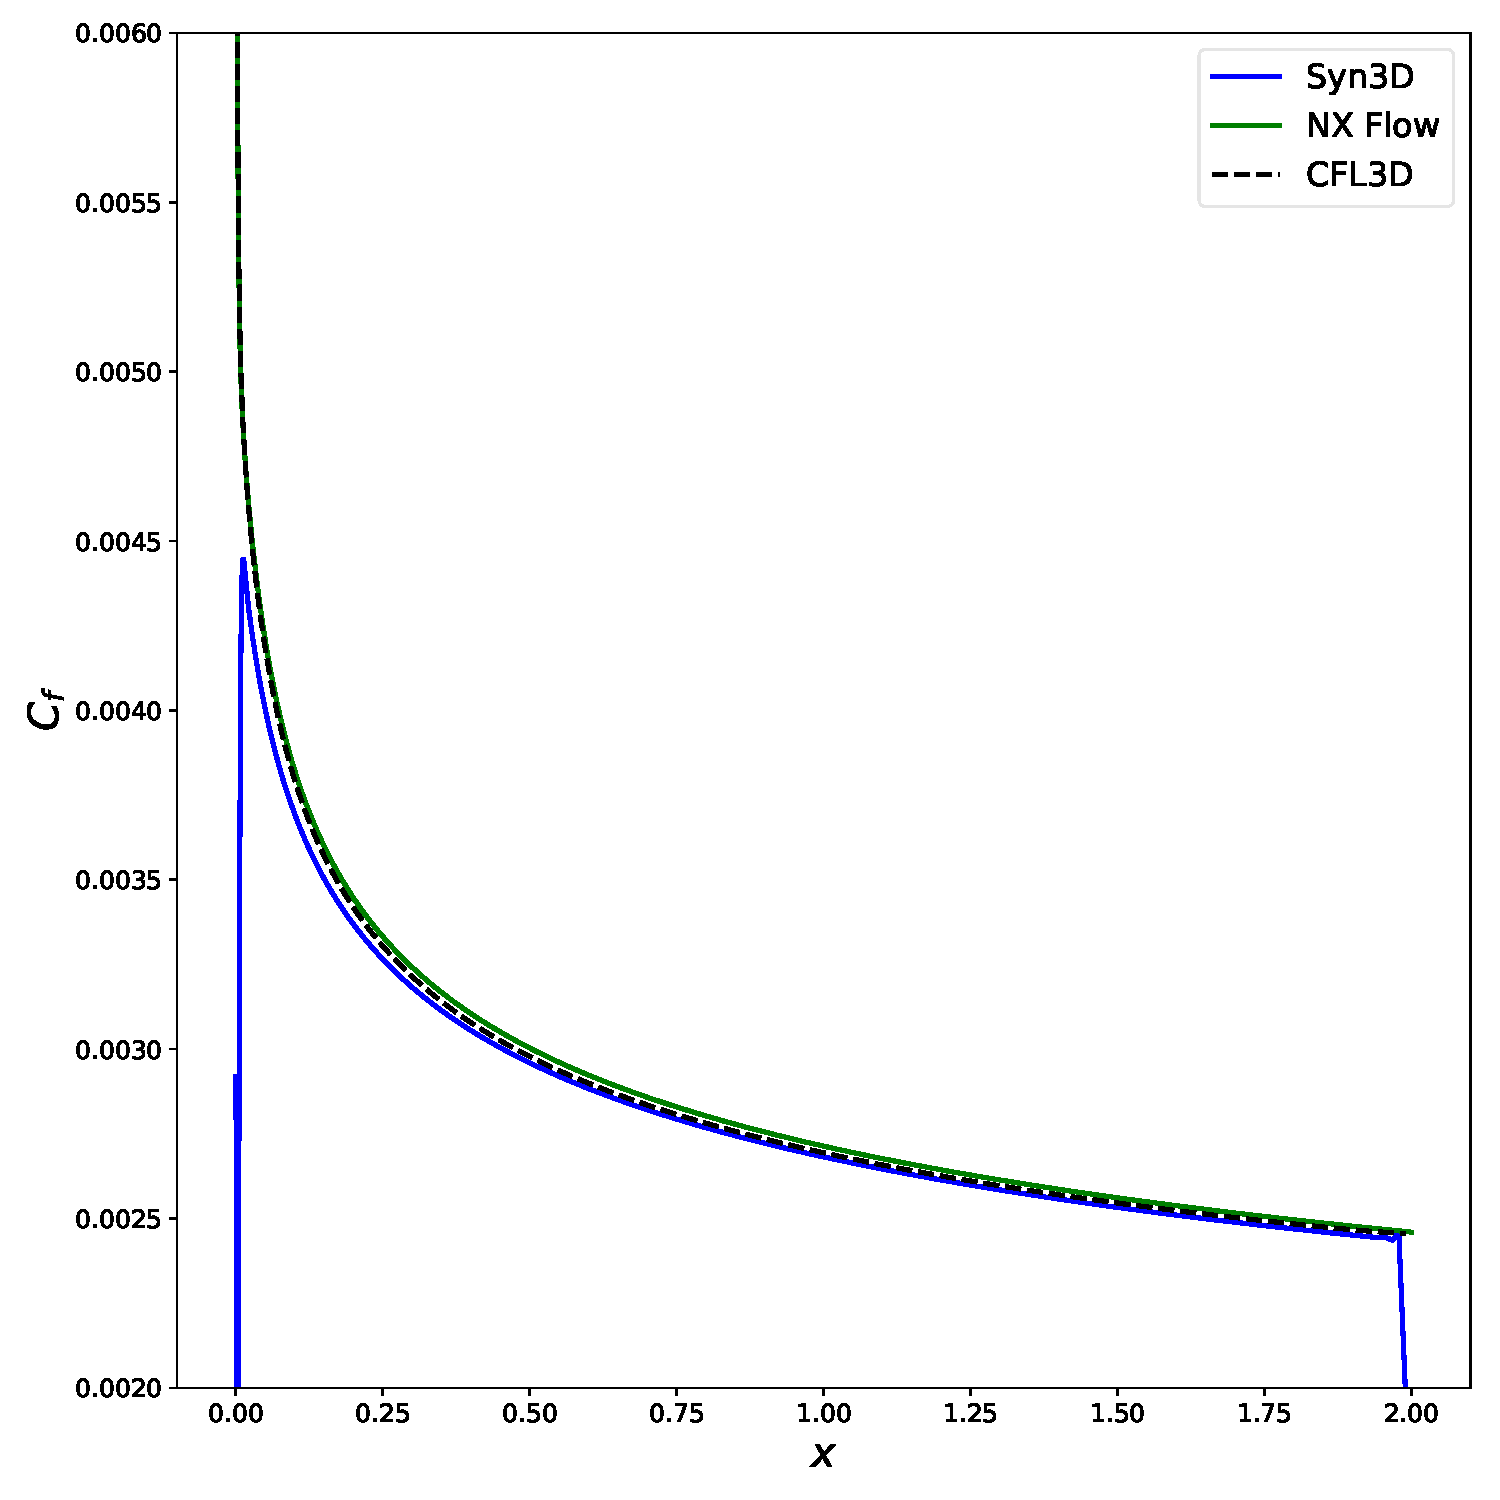
\includegraphics[width=0.7\textwidth]{figs/flat/skin_friction.pdf}
    \caption{Flat Plate (syn3D \& NX Flow): Coefficient of skin friction along the plate.}
    \label{fig:flatcf}
\end{figure}

\begin{figure}[ht!]
\centering
\begin{subfigure}{.32\textwidth}
  \centering
  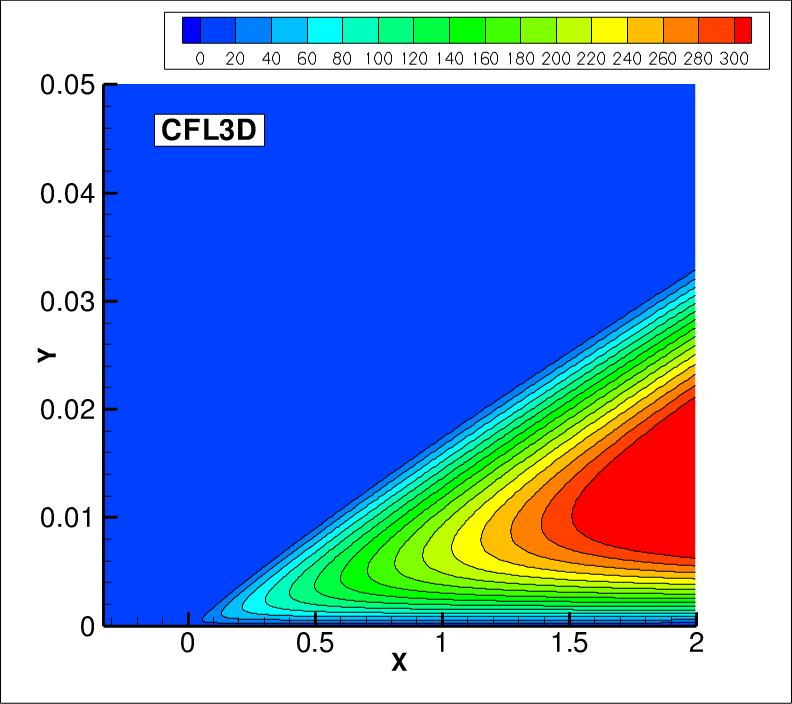
\includegraphics[width=1.0\textwidth]{figs/flat/mut_contours_cfl3d.jpg}
  \caption{CFL3D}
\end{subfigure}%
\begin{subfigure}{.32\textwidth}
  \centering
  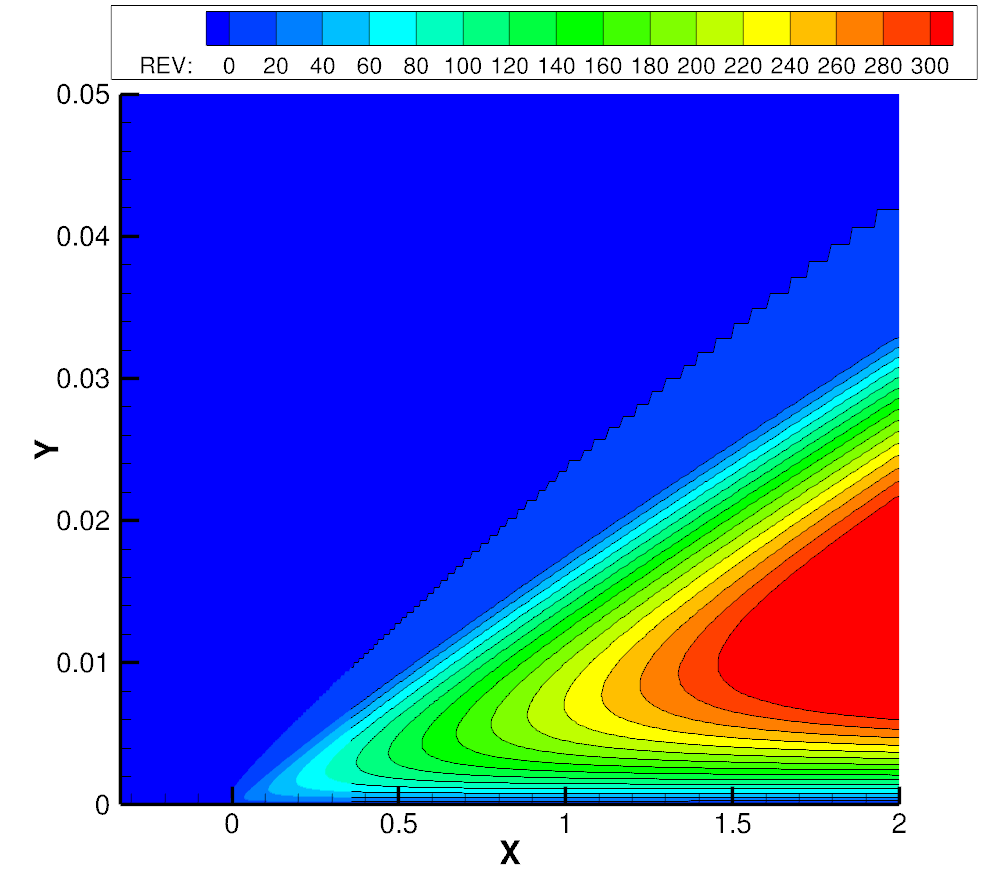
\includegraphics[width=1.0\textwidth]{figs/flat/rev_sa.png}
  \caption{syn3D}
\end{subfigure}
\begin{subfigure}{.32\textwidth}
  \centering
  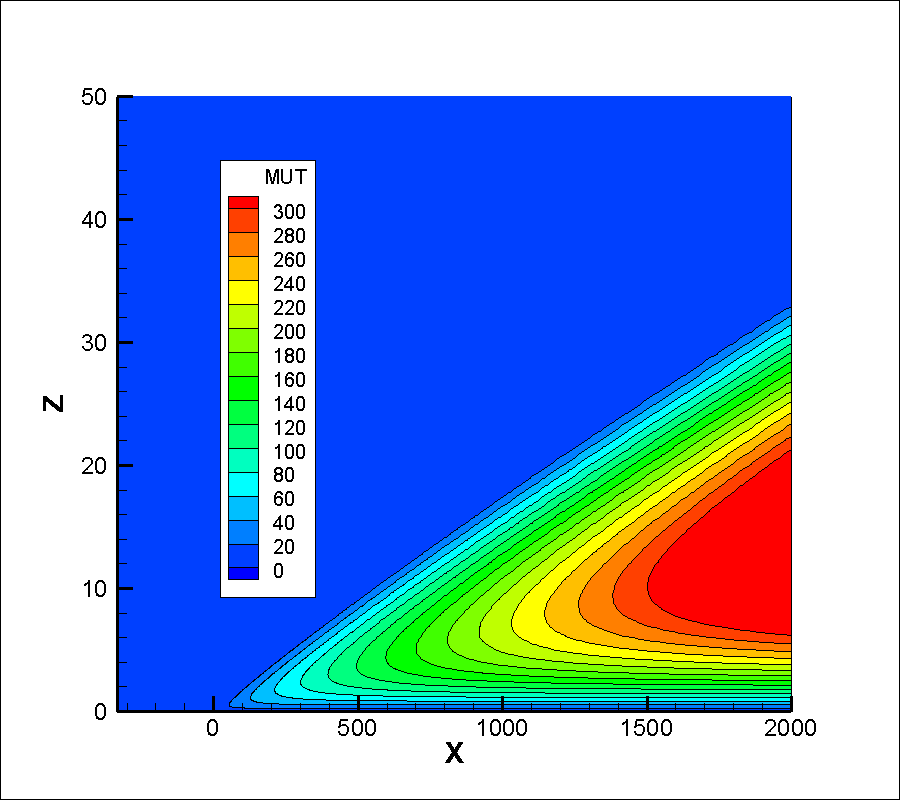
\includegraphics[width=1.0\textwidth]{figs/flatnx/mut_contour.png}
  \caption{NX Flow}
\end{subfigure}
\caption{Flat Plate (syn3D \& NX Flow): Contours of non-dimensionalized eddy viscosity}
\label{fig:flatmutcontour}
\end{figure}

\begin{figure}[ht!]
\centering
\begin{subfigure}{.45\textwidth}
  \centering
  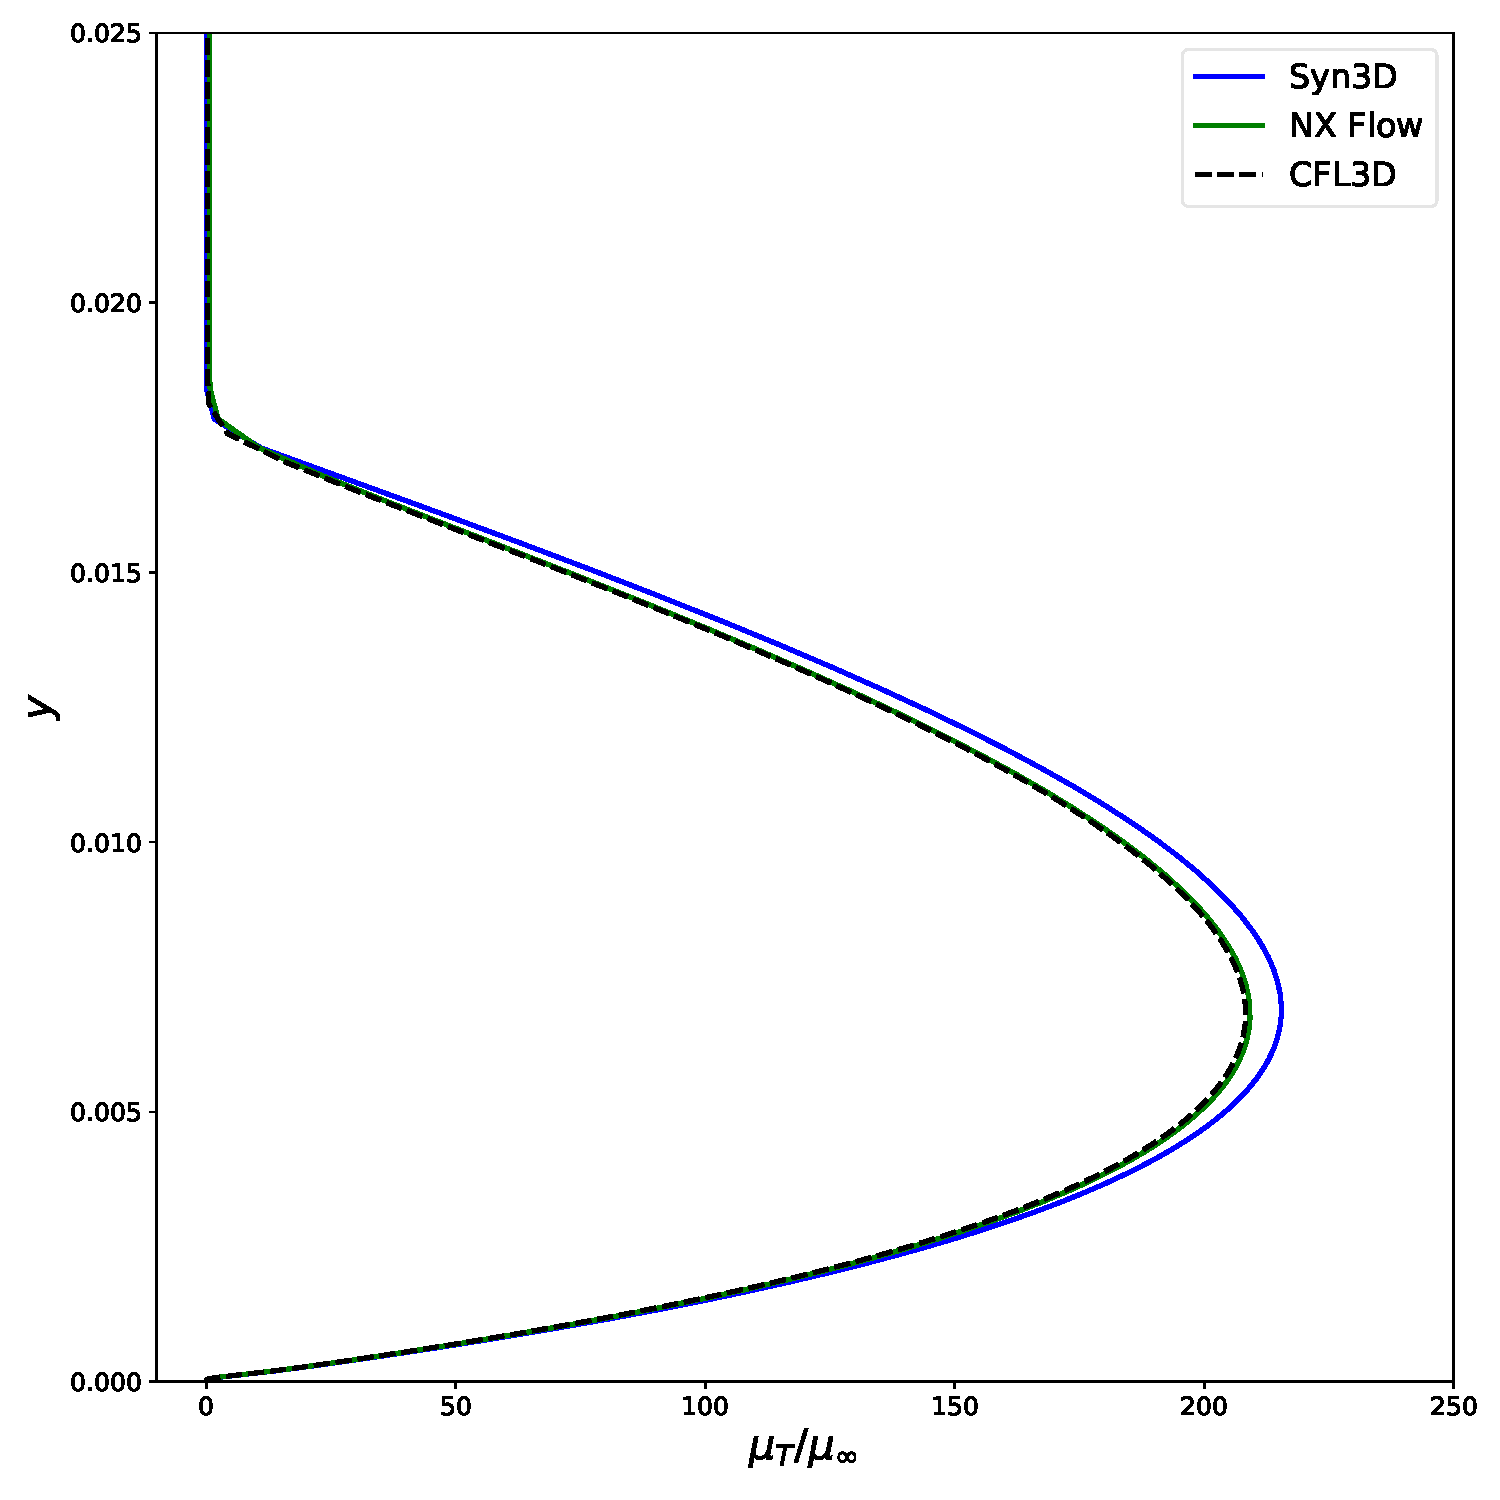
\includegraphics[width=1.0\textwidth]{figs/flat/mut_x097.pdf}
  \caption{Nondimensional eddy viscosity at x=0.97 }
\end{subfigure}%
\begin{subfigure}{.45\textwidth}
  \centering
  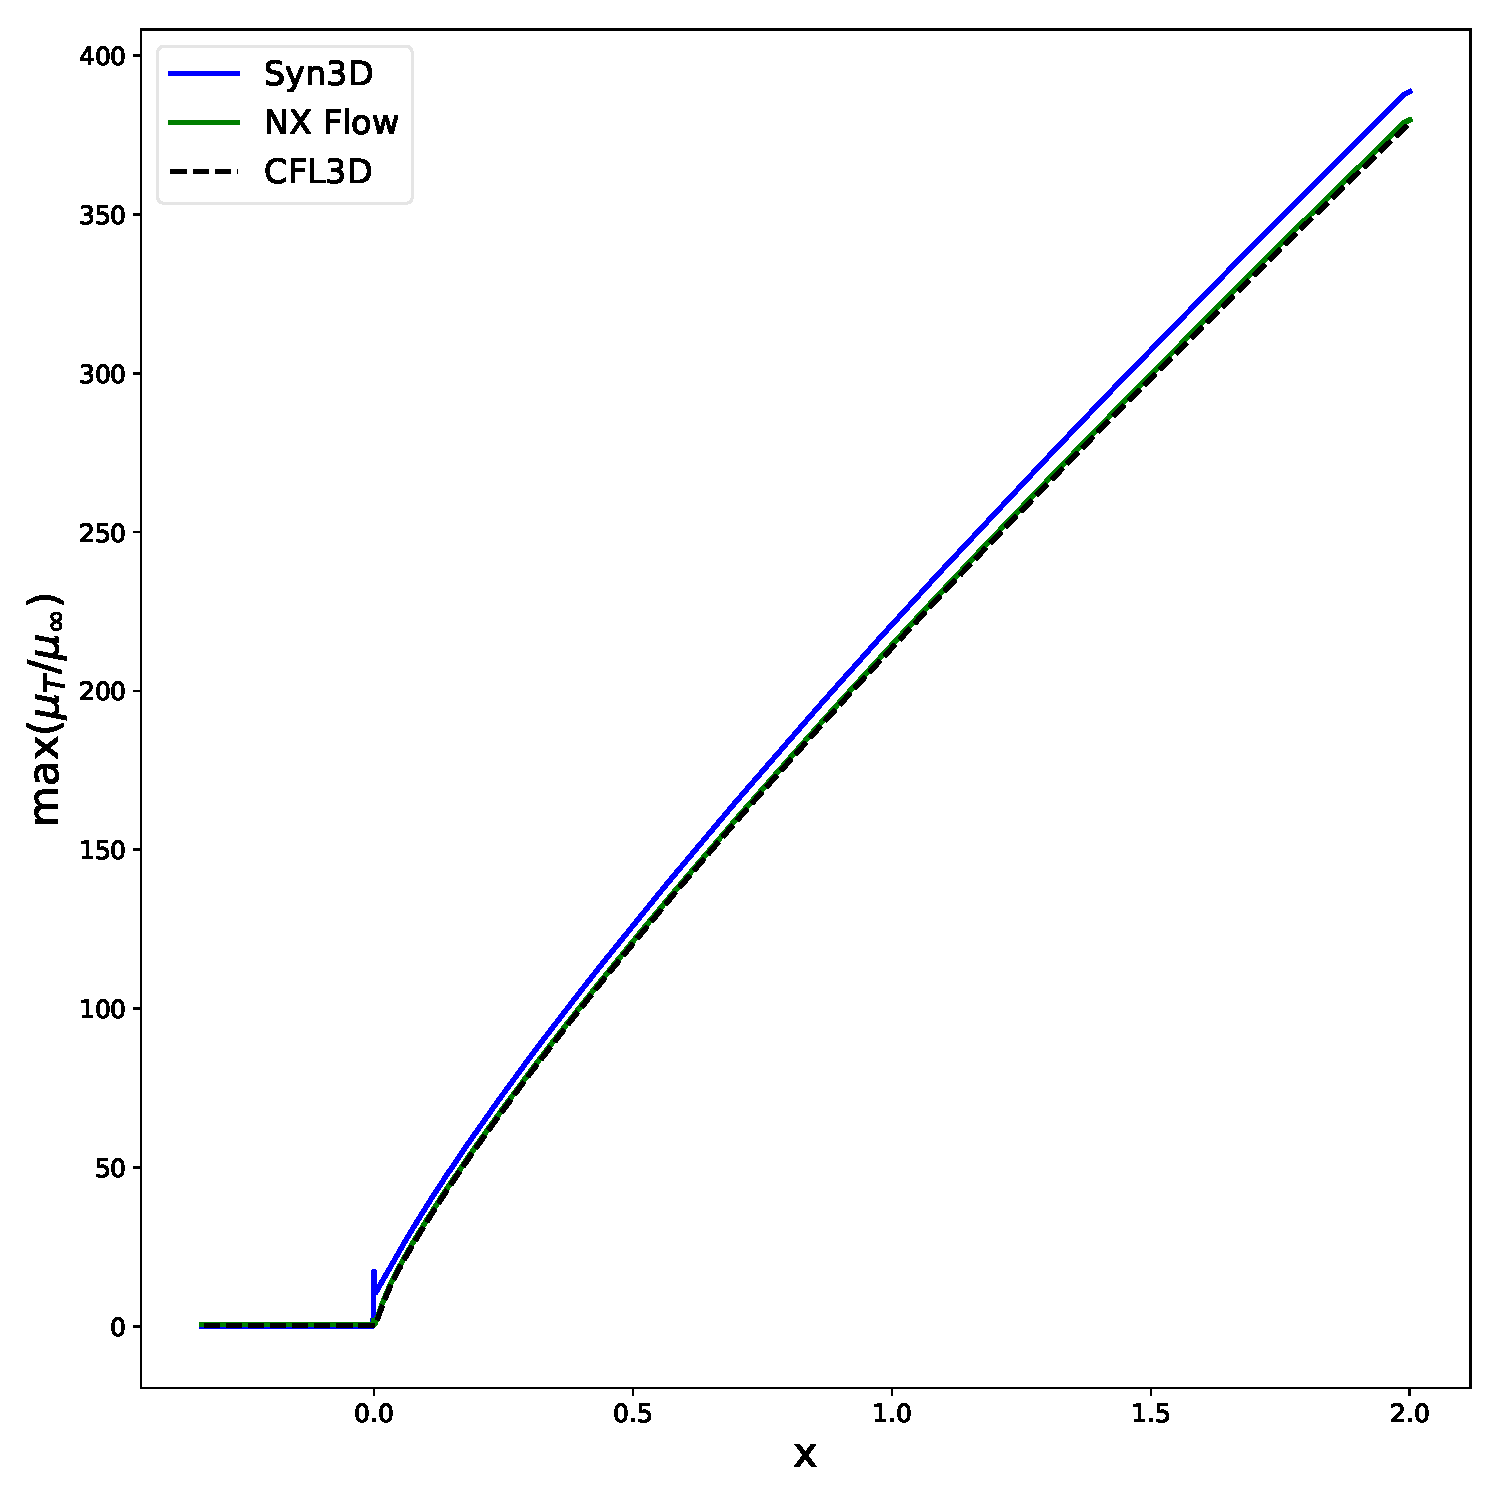
\includegraphics[width=1.0\textwidth]{figs/flat/maxmut.pdf}
  \caption{Maximum $\frac{\mu_t}{\mu_{\infty}}$ in the boundary layer}
  \label{fig:flatmutmax}
\end{subfigure}
\caption{Flat Plate (syn3D \& NX Flow): Dimensionless eddy viscosity line plots}
\label{fig:flatmu}
\end{figure}

\begin{figure}[ht!]
\centering
\begin{subfigure}{.45\textwidth}
  \centering
  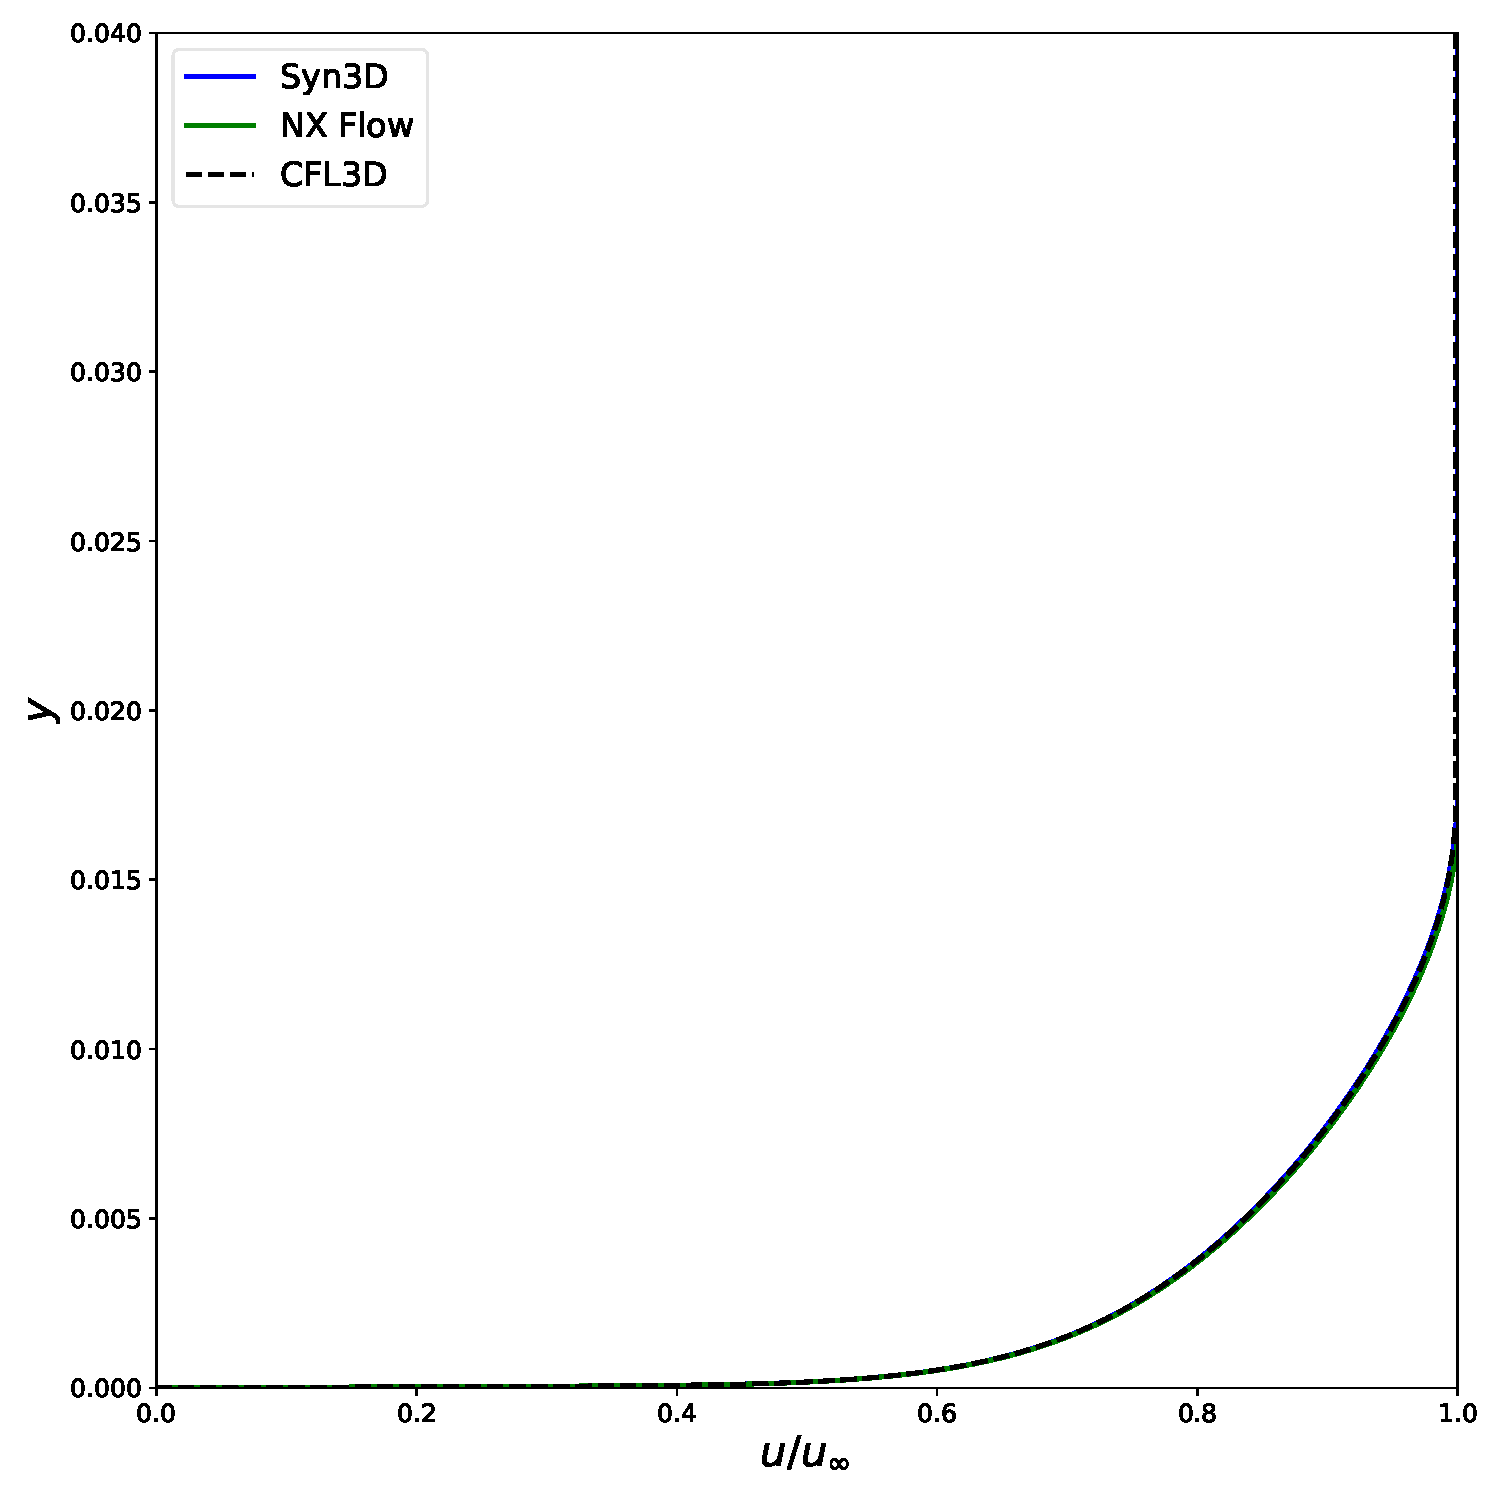
\includegraphics[width=1.0\textwidth]{figs/flat/u097.pdf}
  \caption{$x=0.97$}
\end{subfigure}%
\begin{subfigure}{.45\textwidth}
  \centering
  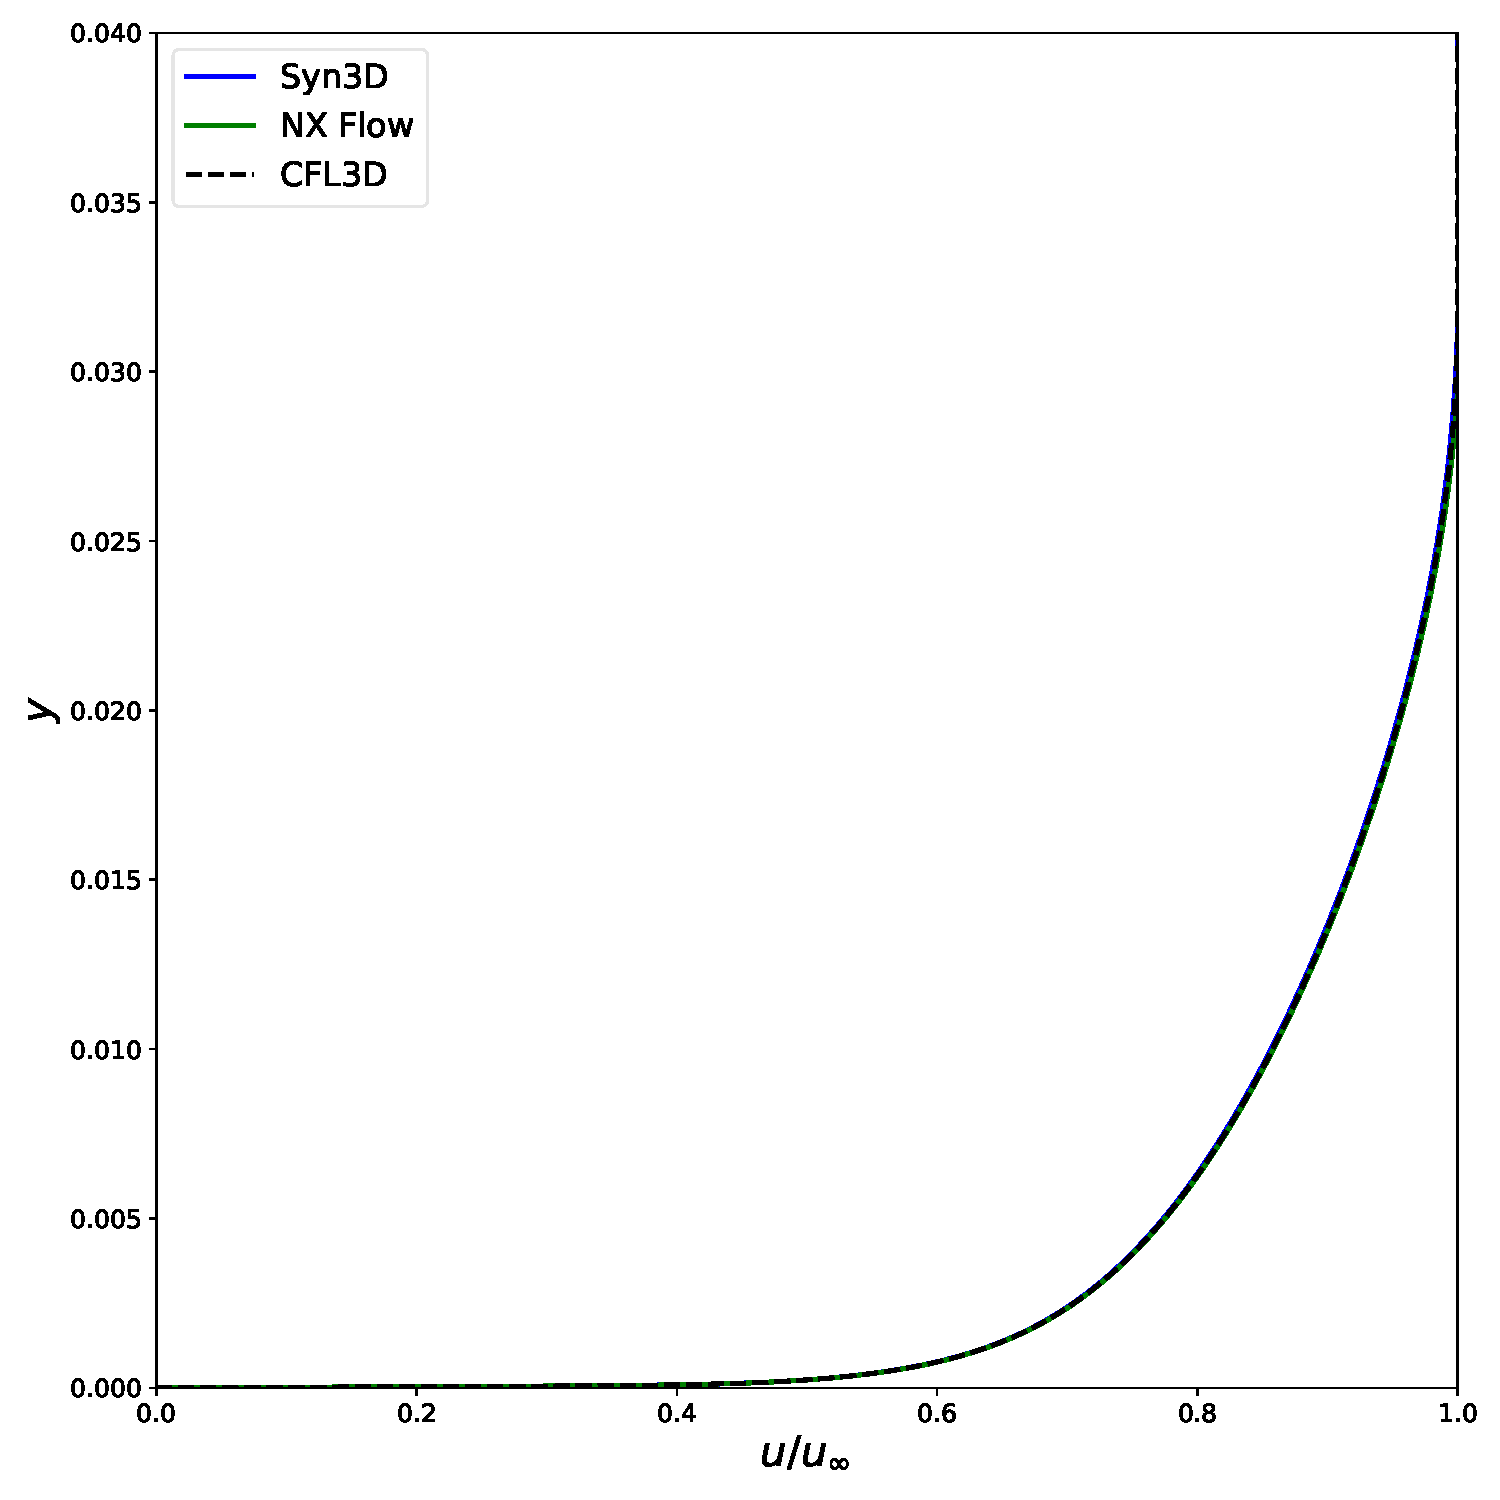
\includegraphics[width=1.0\textwidth]{figs/flat/u190.pdf}
  \caption{$x=1.90$}
\end{subfigure}
\caption{Flat Plate (syn3D \& NX Flow): $\frac{U}{U_{\infty}}$ profiles in the boundary layer}
\label{fig:flatu}
\end{figure}

\begin{figure}[ht!]
\centering
\begin{subfigure}{.45\textwidth}
  \centering
  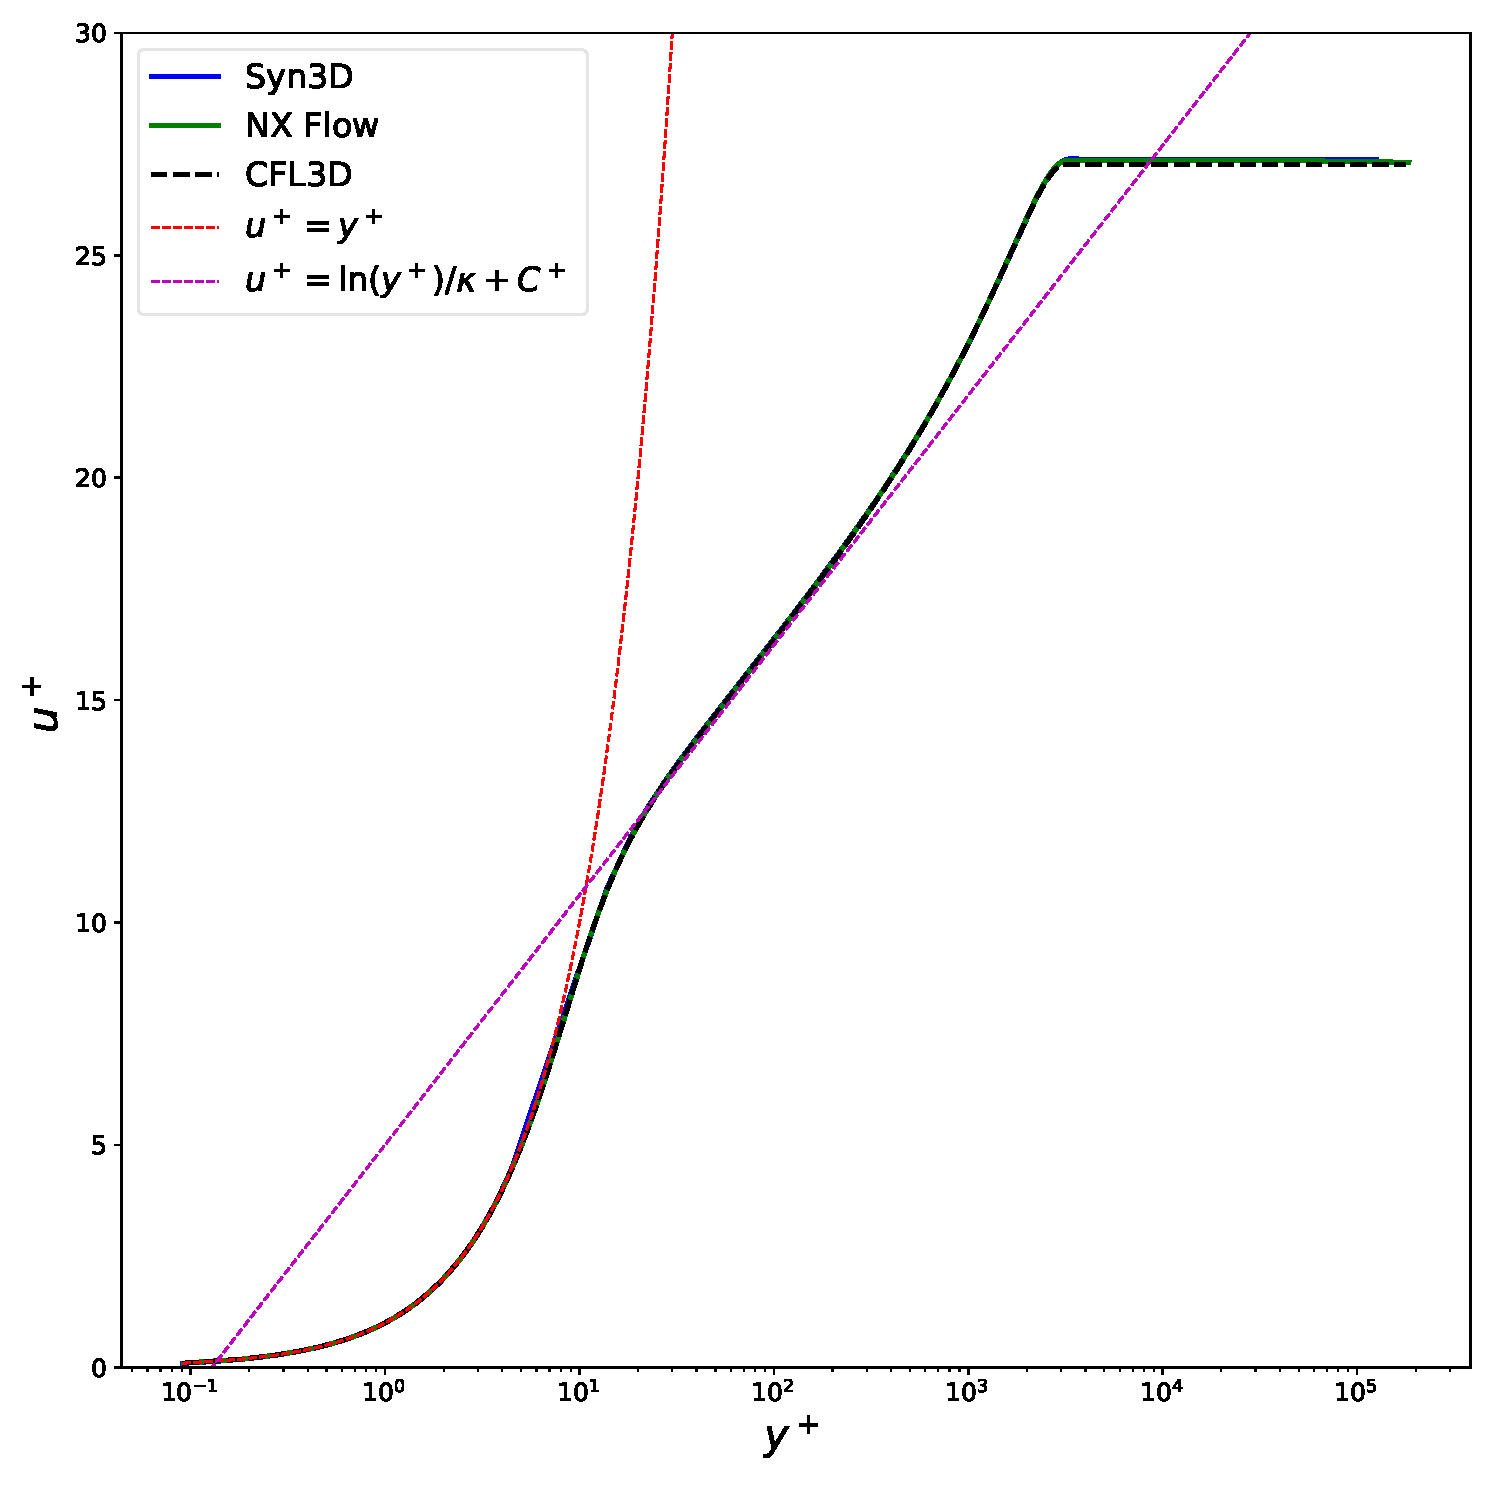
\includegraphics[width=1.0\textwidth]{figs/flat/uplus_yplus_097.pdf}
  \caption{$x=0.97$}
\end{subfigure}%
\begin{subfigure}{.45\textwidth}
  \centering
  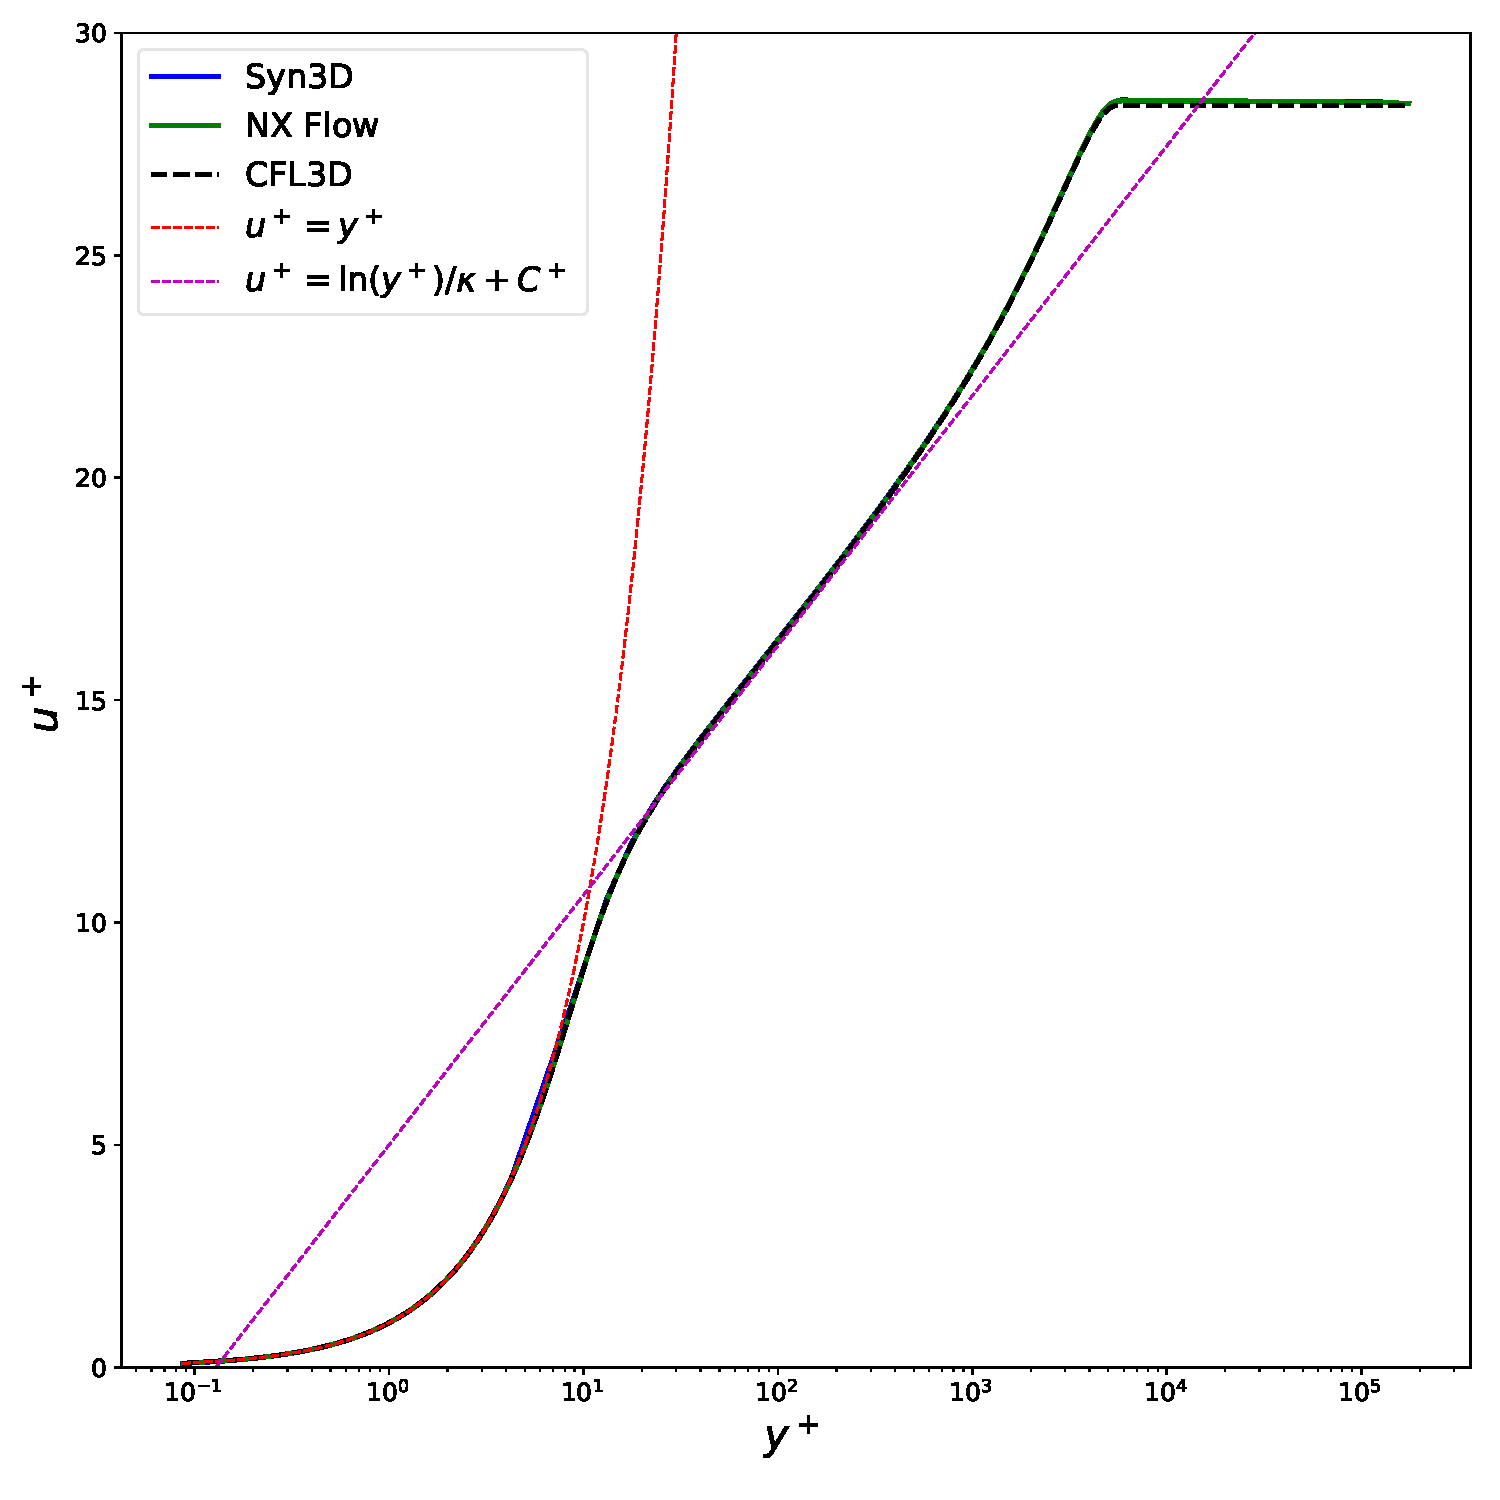
\includegraphics[width=1.0\textwidth]{figs/flat/uplus_yplus_190.pdf}
  \caption{$x=1.90$}
\end{subfigure}
\caption{Flat Plate (syn3D \& NX Flow): $u^+$ vs. $y^+$ profiles in the boundary layer. Law of the wall is also shown for comparison.}
\label{fig:flatupyp}
\end{figure}

\Cref{fig:flatforcestudy} shows the dependence of $C_D$ and $C_f$ on the grid spacing $h = 1/N^2$, where $N$ is the number of grid points. It can be seen that there is still significant differences in results between the second finest and finest grid for syn3D as compared to CFL3D and FUN3D -- the latter is a vertex-centered code also developed by NASA. Thus, syn3D may not have reached the asymptotic range of convergence. Moreover, the importance of a grid study can be seen from these plots: whereas results on the fine grid are mostly similar, they are quite different on the coarser grids, with some being over-predicted and others under-predicted compared to the asymptotic values.

The skin friction coefficient obtained by NX Flow is closer to that of FUN3D run in incompressible mode, which is higher than the compressible value. This explains the over-prediction in the skin friction coefficient as well as drag.

\Cref{fig:synflatcfstudy,fig:synflatprofilestudy} show the variation of skin friction coefficient along the plate and profiles of eddy viscosity and velocity with grid size respectively with syn3D and \Cref{fig:nxflatcfstudy,fig:nxflatprofilestudy} show the variation with NX Flow. These plots show that the solution field seems to converge to a unique solution, as opposed to oscillating back and forth between different values. As expected, solutions on coarser grids display increased dissipation; the discretization errors scale with the grid spacing and typically lead to increased diffusion. Moreover, the artificial dissipation parameters in syn3D were not tuned for each individual grid, and they lead to significantly increased dissipation on coarser grids. Nevertheless, the grid study provides an ability to determine the minimum required grid size to ensure sufficiently accurate values of the drag coefficient to within five drag counts. In the case of NX Flow, the $35\times25$ grid was required, while syn3D demanded a grid of $69\times49$. A study of the choice of artificial dissipation may reduce the grid density requirement, however, this was not part of the work.
\begin{figure}[ht!]
\centering
\begin{subfigure}{.45\textwidth}
  \centering
  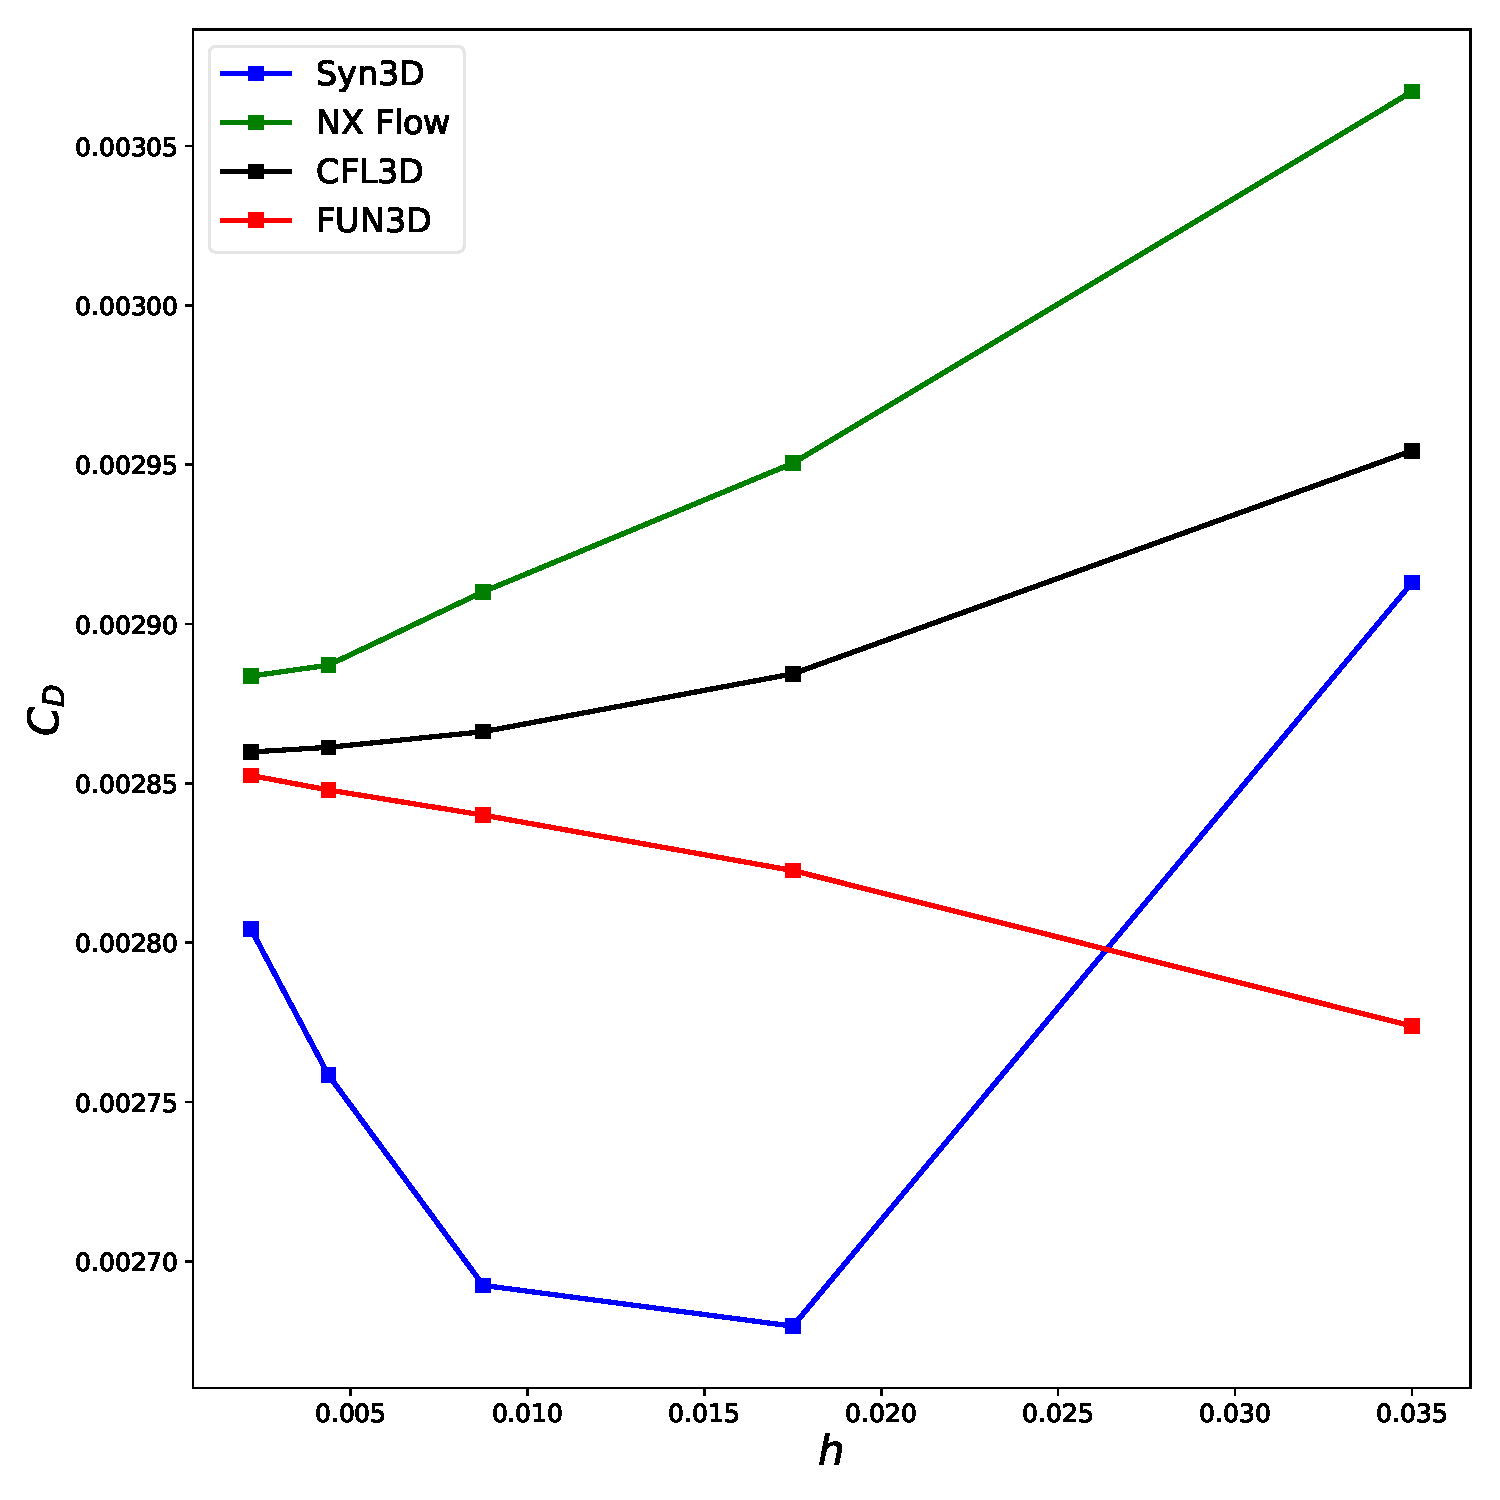
\includegraphics[width=1.0\textwidth]{figs/flat/cd_grid.pdf}
  \caption{Coefficient of drag.}
\end{subfigure}%
\begin{subfigure}{.45\textwidth}
  \centering
  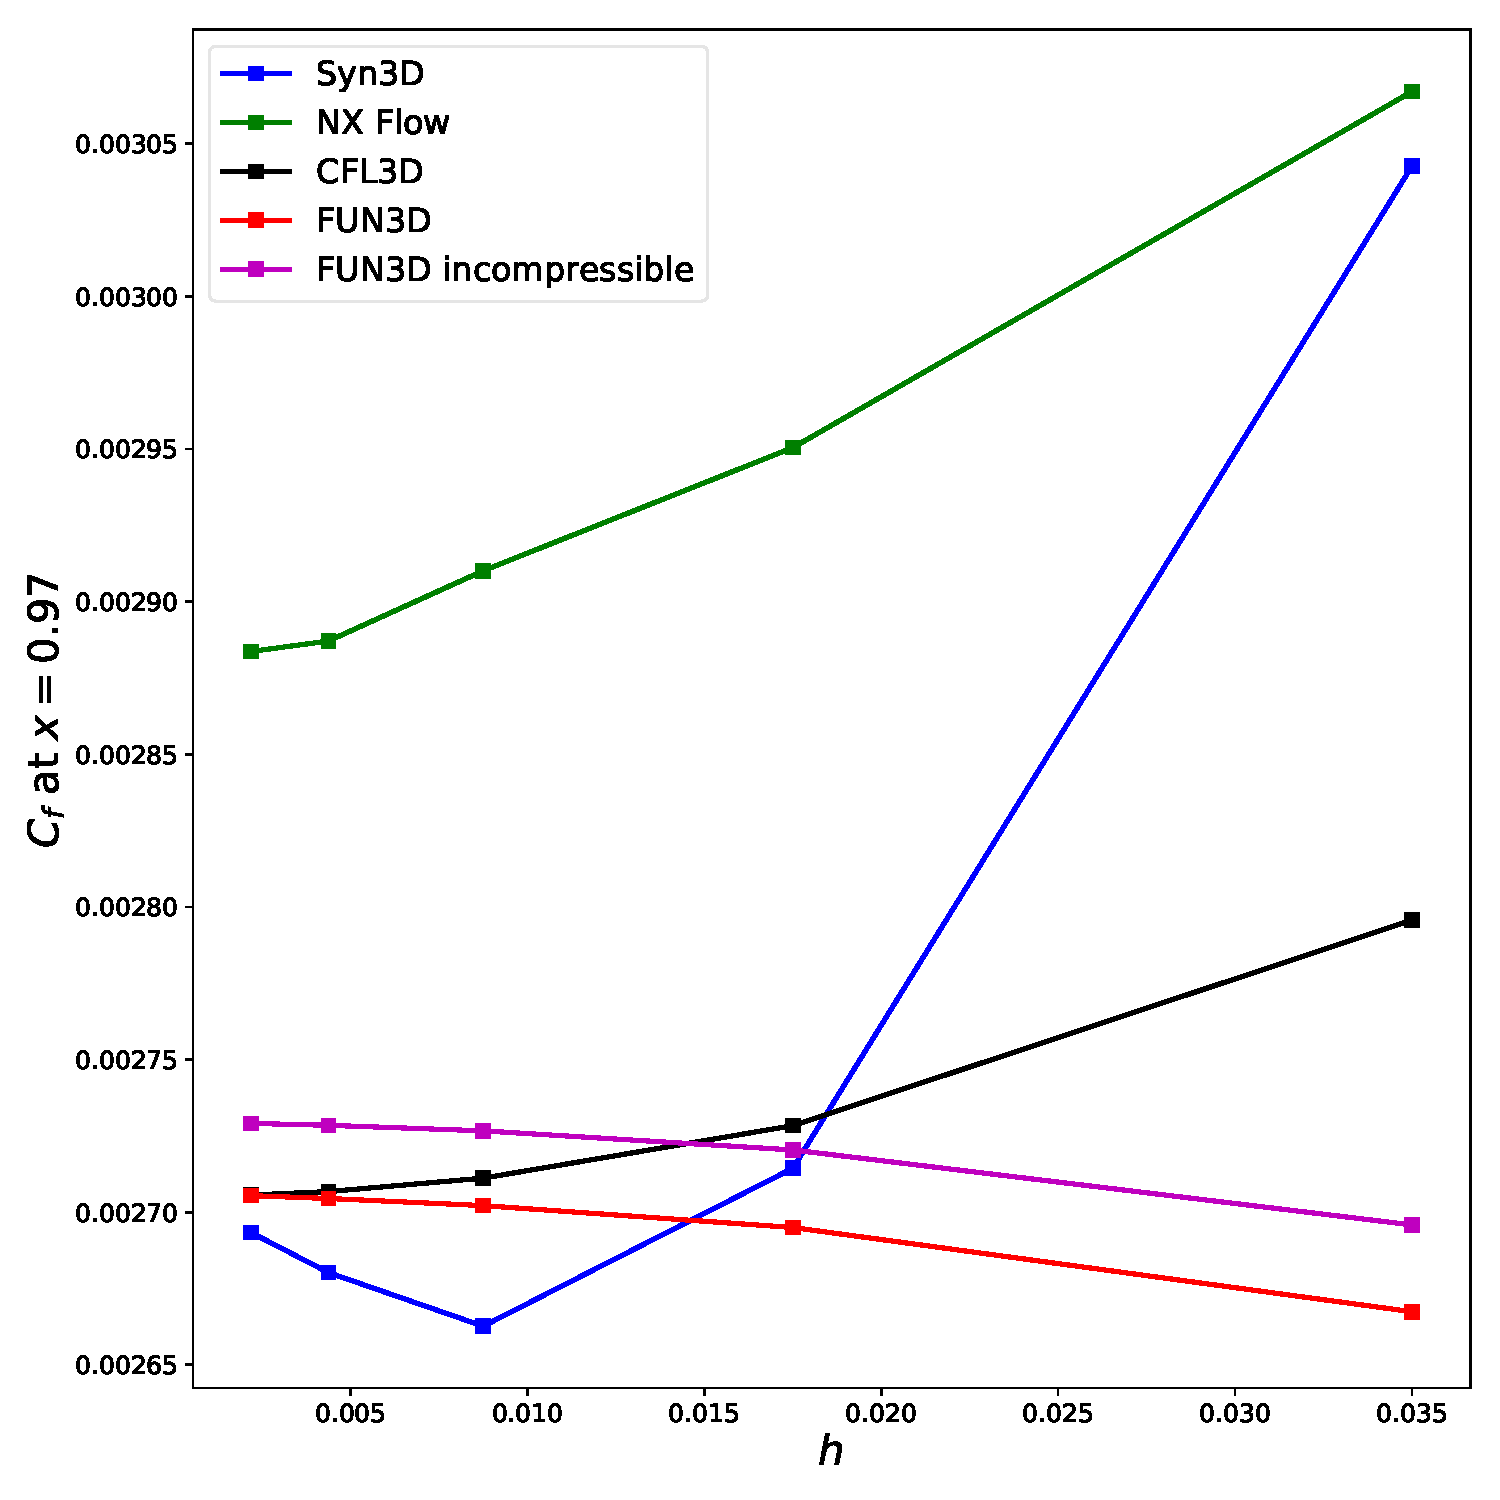
\includegraphics[width=1.0\textwidth]{figs/flat/cf_grid.pdf}
  \caption{Coefficient of Skin Friction at x=0.97.}
\end{subfigure}
\caption{Flat Plate (syn3D): Force coefficients for various grid sizes.}
\label{fig:flatforcestudy}
\end{figure}

\begin{figure}[ht!]
\centering
  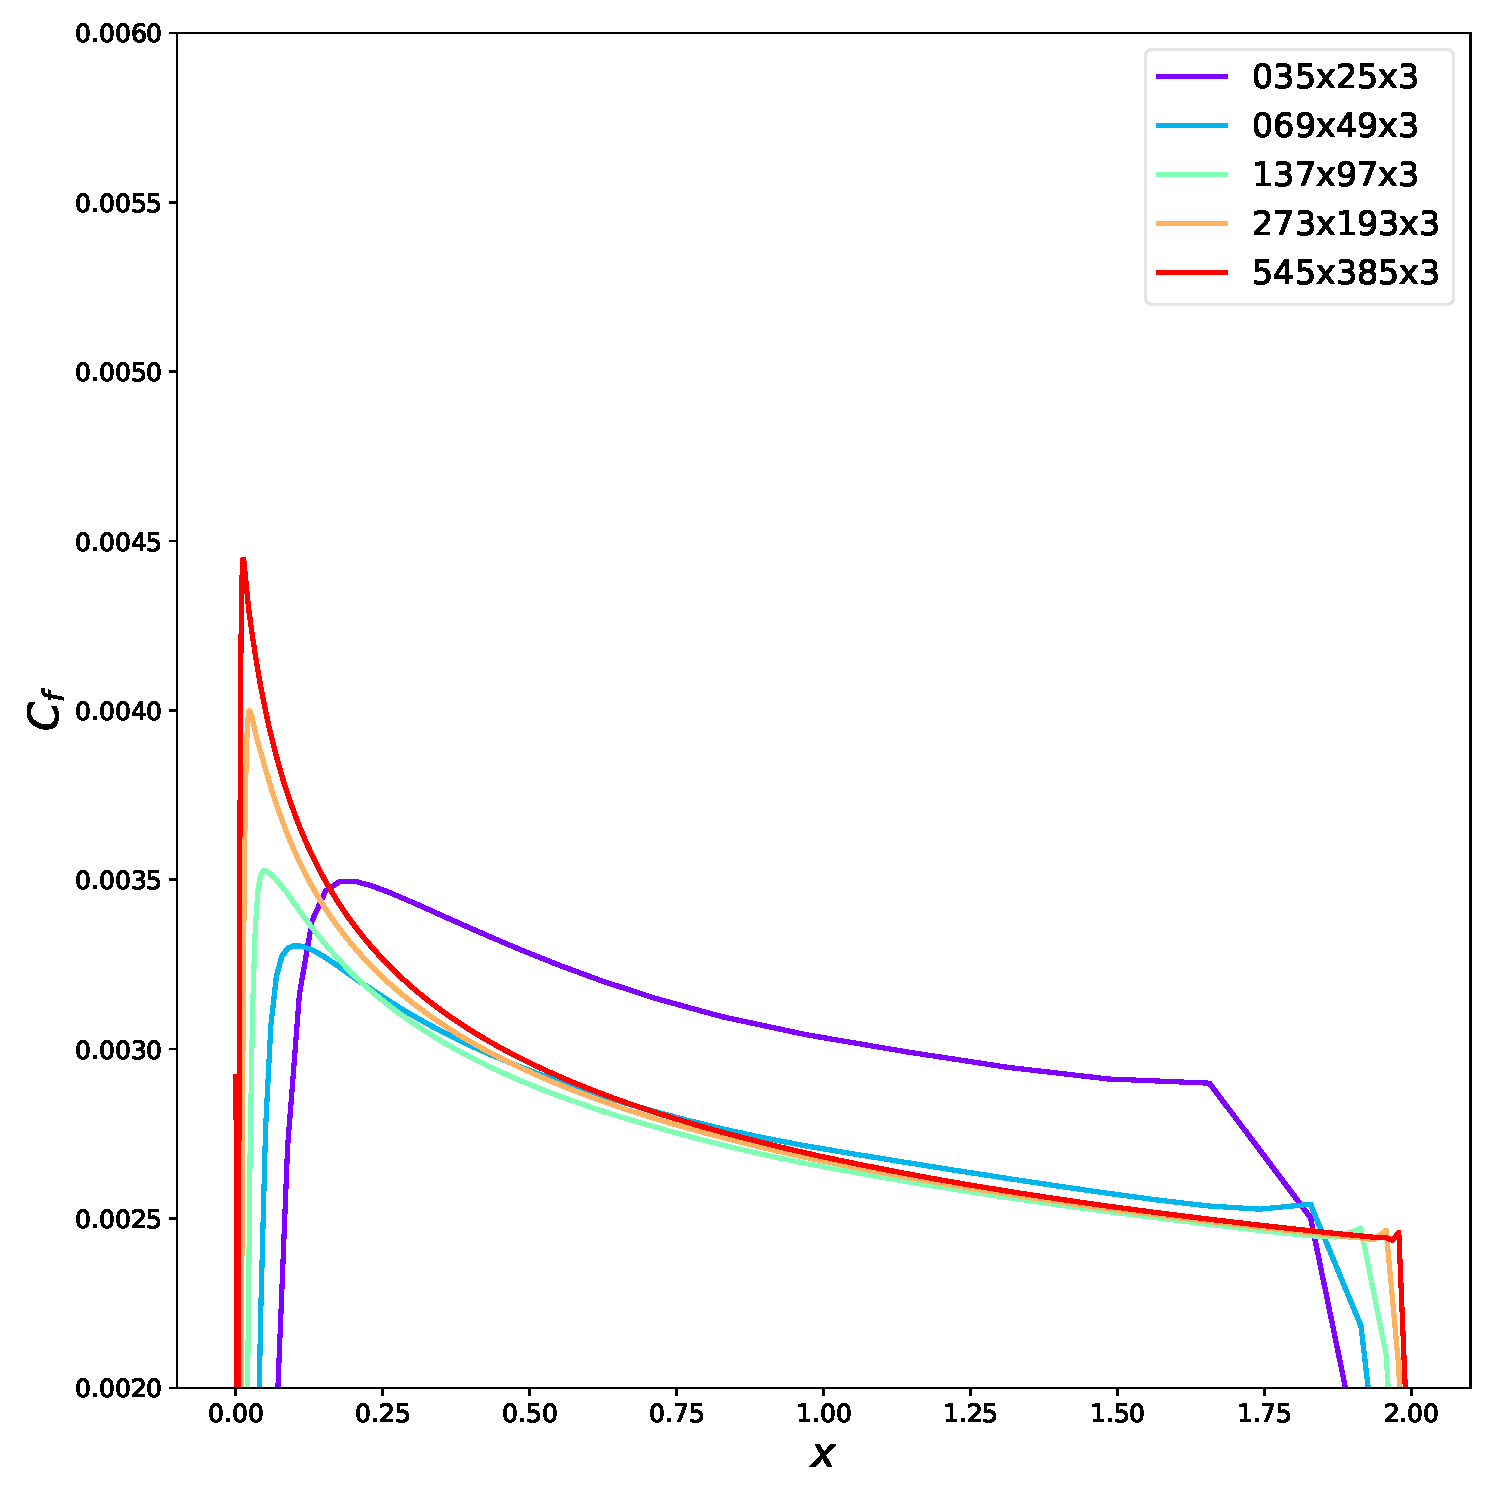
\includegraphics[width=0.7\textwidth]{figs/flat/skin_friction_grid.pdf}
  \caption{Flat Plate (syn3D): Coefficient of skin friction on various grids.}
  \label{fig:synflatcfstudy}
\end{figure}

\begin{figure}[ht!]
\centering
\begin{subfigure}{.45\textwidth}
  \centering
  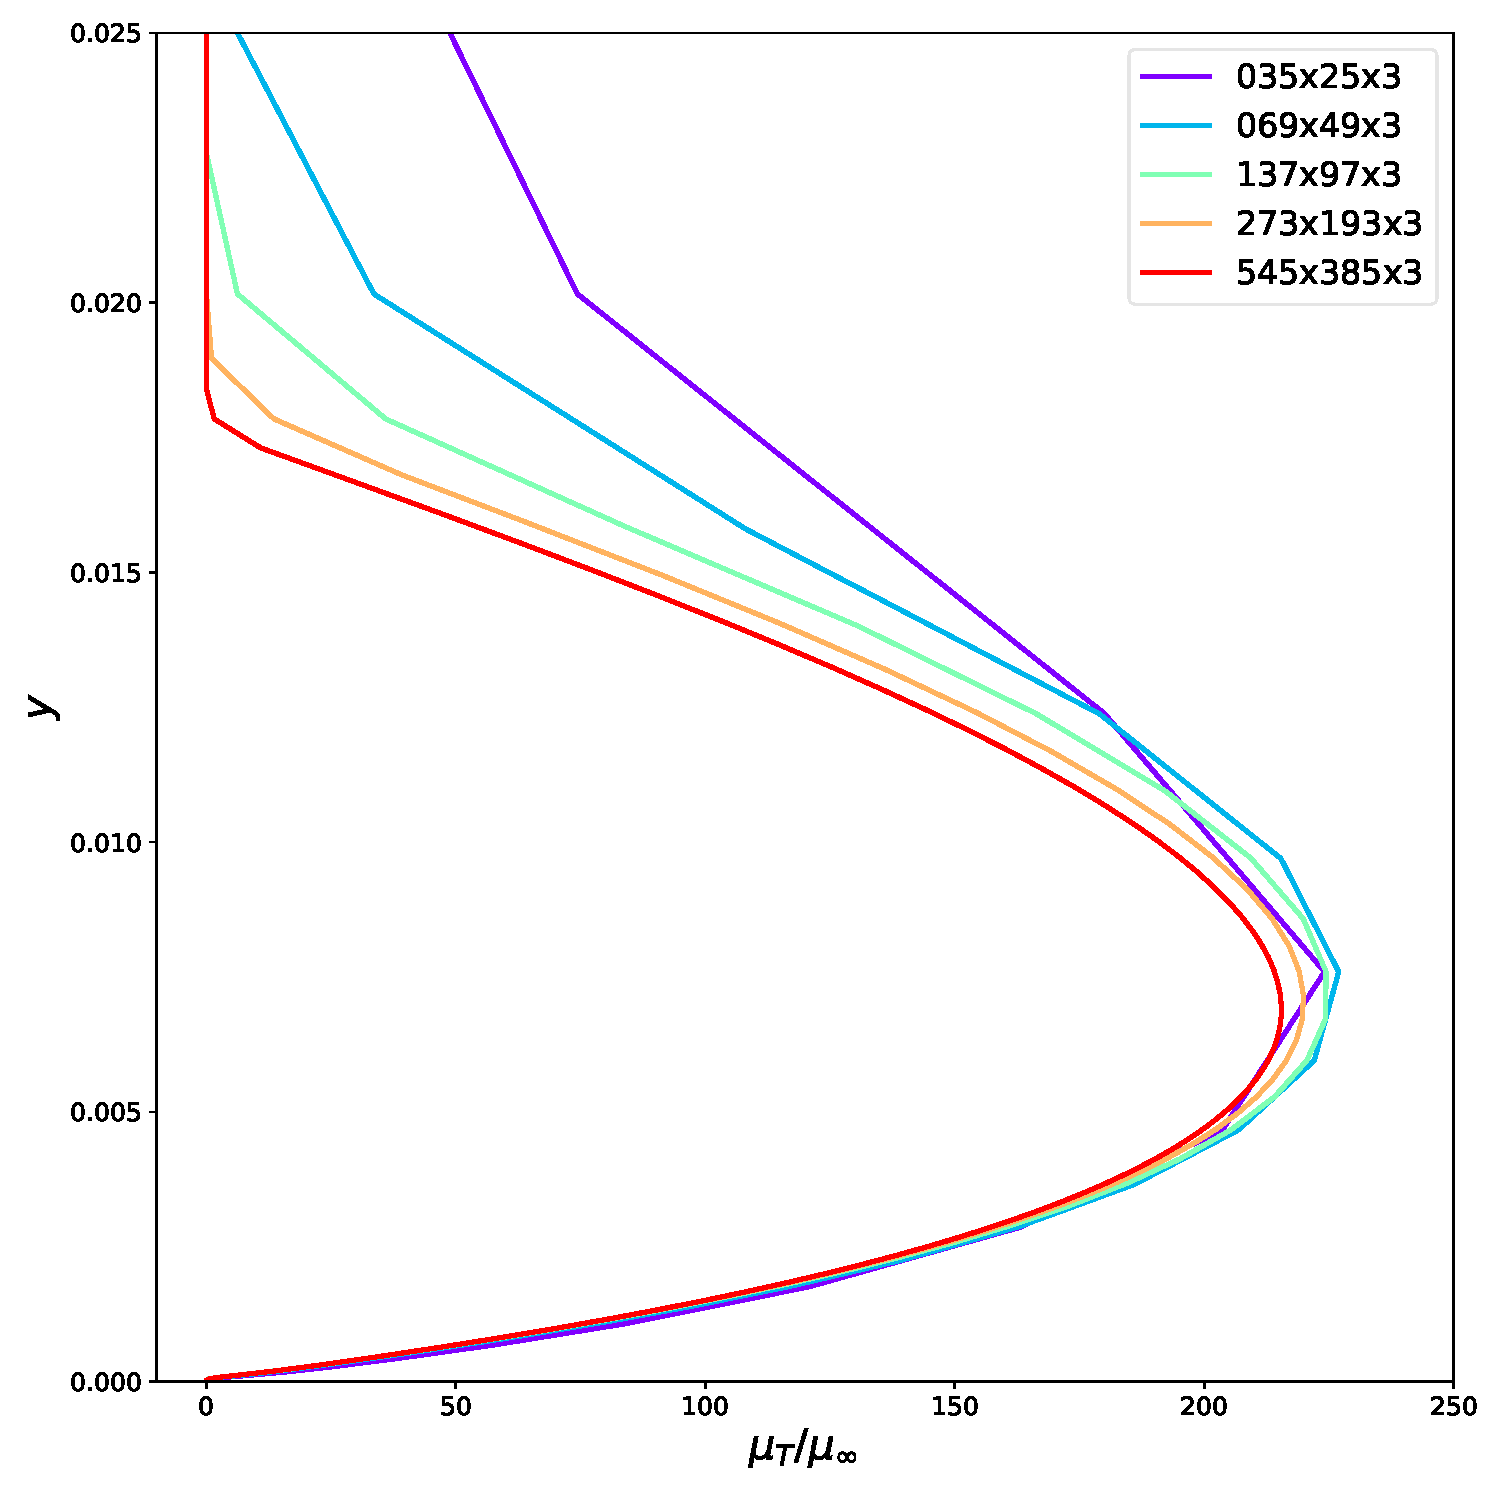
\includegraphics[width=1.0\textwidth]{figs/flat/rev_grid.pdf}
  \caption{Dimensionless eddy viscosity}
\end{subfigure}%
\begin{subfigure}{.45\textwidth}
  \centering
  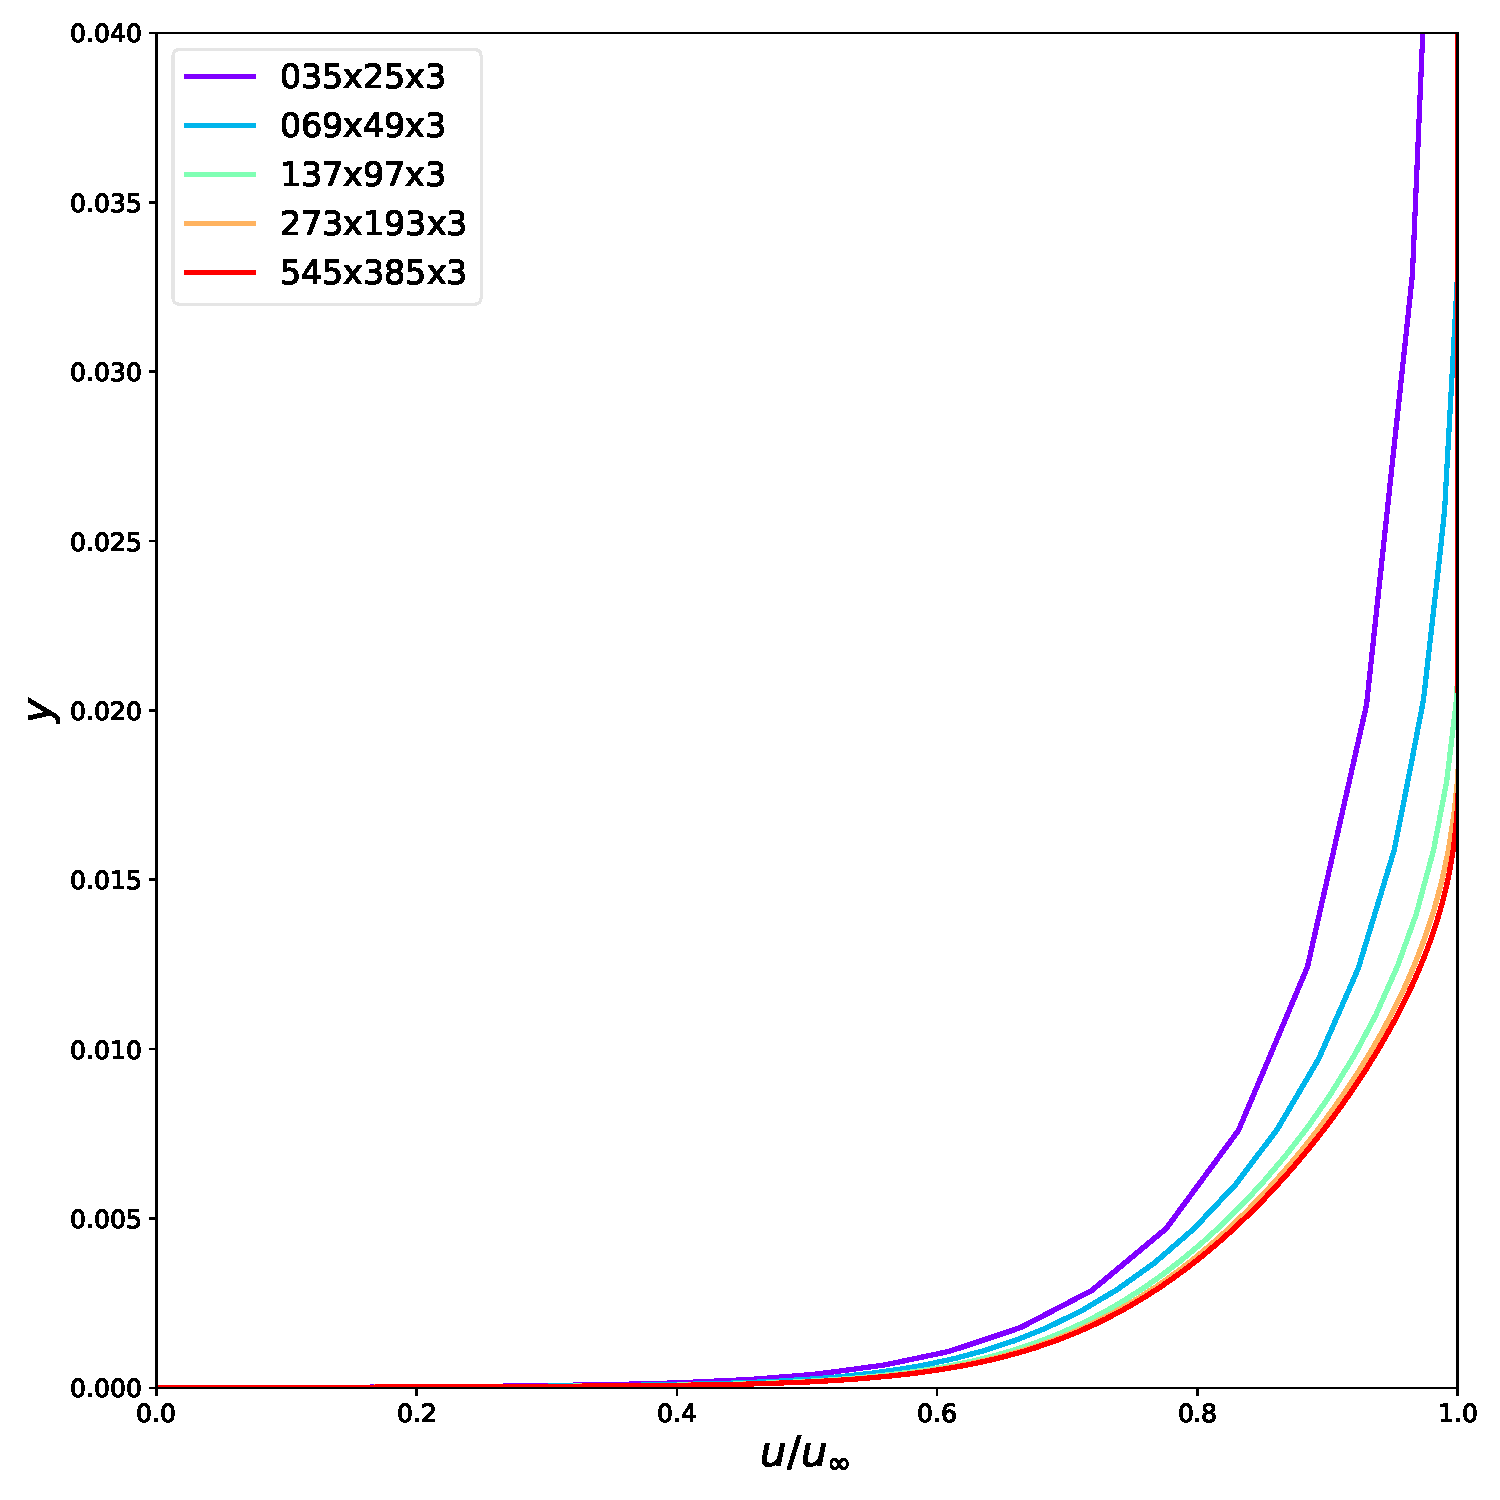
\includegraphics[width=1.0\textwidth]{figs/flat/u097_grid.pdf}
  \caption{Dimensionless velocity}
\end{subfigure}
\caption{Flat Plate (syn3D): Profiles at $x=0.97$ for various grid sizes.}
\label{fig:synflatprofilestudy}
\end{figure}

\begin{figure}[ht!]
\centering
  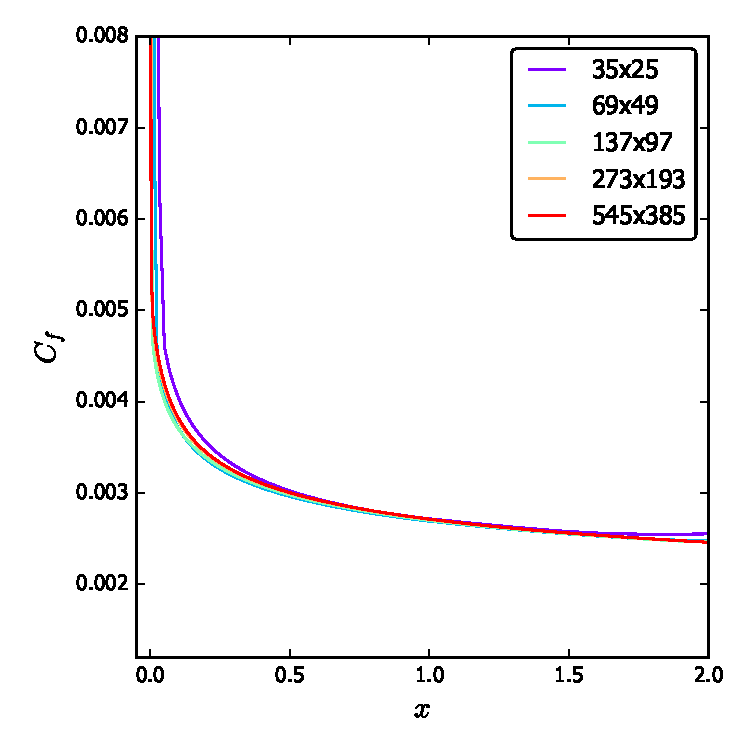
\includegraphics[width=0.7\textwidth]{figs/flatnx/cf_gridstudy.pdf}
  \caption{Flat Plate (NX Flow): Coefficient of skin friction on various grids.}
  \label{fig:nxflatcfstudy}
\end{figure}

\begin{figure}[ht!]
\centering
\begin{subfigure}{.45\textwidth}
  \centering
  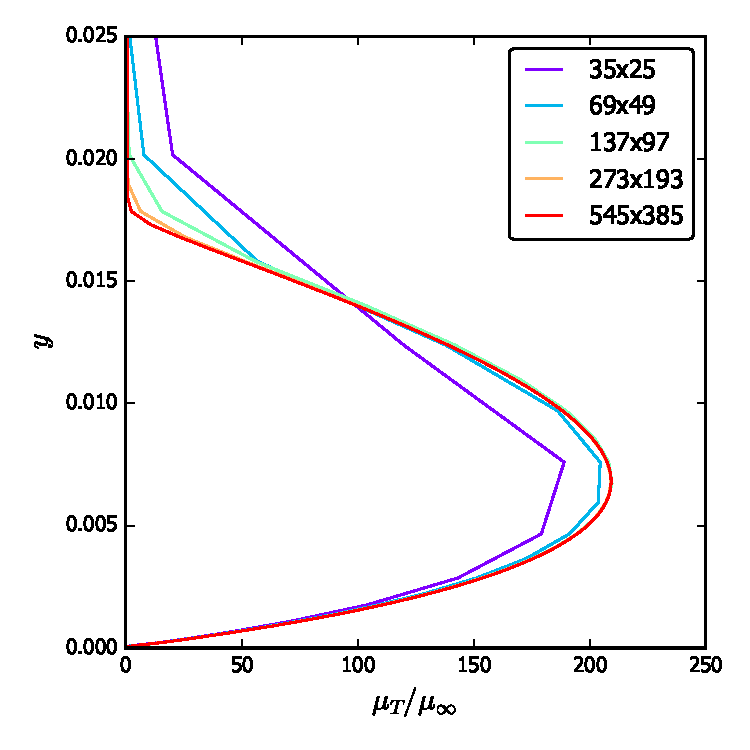
\includegraphics[width=1.0\textwidth]{figs/flatnx/mut_gridstudy.pdf}
  \caption{Dimensionless eddy viscosity}
\end{subfigure}%
\begin{subfigure}{.45\textwidth}
  \centering
  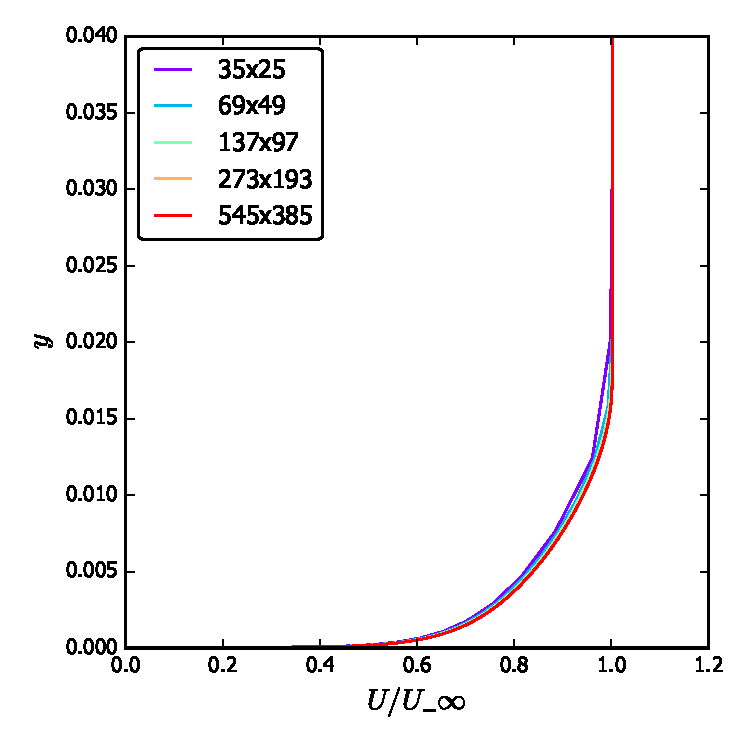
\includegraphics[width=1.0\textwidth]{figs/flatnx/u_x097_gridstudy.pdf}
  \caption{Dimensionless velocity}
\end{subfigure}
\caption{Flat Plate (NX Flow): Profiles at $x=0.97$ for various grid sizes.}
\label{fig:nxflatprofilestudy}
\end{figure}

\section{Two-dimensional bump-in-channel}
Upon completion of the validation of the flow over a flat-plate, the turbulent flow on a two-dimensional bump-in-channel case was investigated. This case is also available on~\cite{tmr} under the name ``2D Bump-in-channel''. This case was only run with syn3D.

The problem domain and flow conditions are shown in~\Cref{fig:2dbump}. It is referred to as two-dimensional due to the shape of the bump not depending upon the $z$ coordinate, as opposed to the three-dimensional bump in~\Cref{sec:syn3dbump}.

This case is different from the previous flat plate case because it involves wall curvature, which induces a pressure gradient. The TMR website also provides five grids for this case.
\begin{figure}
    \centering
    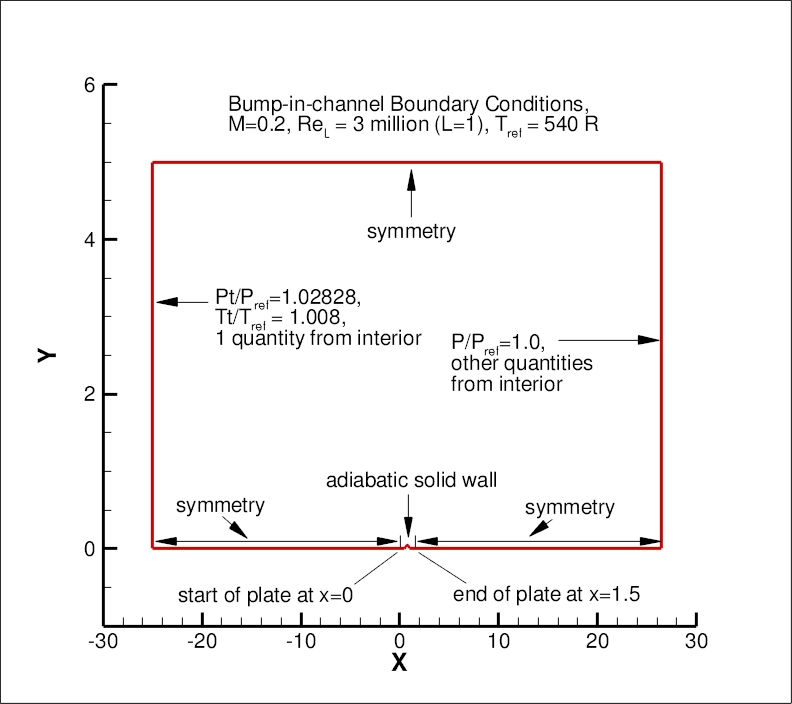
\includegraphics[width=0.7\textwidth]{figs/2dbump/bumpBCpic.jpg}
    \caption{Turbulent two-dimensional bump case~\cite{tmr}.}
    \label{fig:2dbump}
\end{figure}

\begin{table}[ht!]
    \centering
    \caption{2D Bump (syn3D): Comparison of force coefficients for the finest two-dimensional bump.}
\label{tab:syn2dbump1}
\begin{tabular}{@{}lcccc@{}}
\toprule
Solver & $C_L$ & $C_D$ & $C_{Dv}$ & $C_{Dp}$ \\
\midrule
CFL3D & 0.0249 & 0.0036  & 0.0032 & 0.0004  \\
syn3D & 0.0251 &  0.0035 & 0.0031 & 0.0004  \\  \bottomrule
\end{tabular}

\end{table}

\begin{table}[ht!]
\centering
\caption{2D Bump (syn3D): Comparison of skin friction coefficient at various locations.}
\label{tab:syn2dbump2}
\begin{tabular}{lccc}
\toprule
& \multicolumn{3}{c}{$C_f$} \\
\cline{2-4}
Solver & $x=0.75$ & $x=0.6321975$ & $x=0.8678025$ \\
\midrule
CFL3D & 0.00615 & 0.00519  & 0.002680   \\
syn3D & 0.00610 & 0.00519  & 0.002835  \\
\bottomrule
\end{tabular}

\end{table}

\Cref{tab:syn2dbump1} tabulates the drag coefficient, the lift coefficient $C_L$ as well as the contributors to the drag coefficient $C_{Dv}$ and $C_{Dp}$, which represent the contributions due to viscous forces and pressure forces respectively. \Cref{tab:syn2dbump2} tabulates the skin friction coefficient probed at various locations. These tables show good agreement between CFL3D and syn3D.

\Cref{fig:syn2dbumpcnvstudy} shows the convergence for all grids. Reduction of the residual is quite slow for this particular problem, with the finest grid taking over 3 days on 64 processors to complete. In addition, a plateau of the residual at approximately $2\times10^{-3}$ can be observed for the three coarsest grids, which is likely due to the interfaces between the symmetry planes and the solid wall. In fact, the maximum residual occurs at the field points with faces lying on that interface, which is also an interface between block boundaries.
\begin{figure}[ht!]
\centering
\begin{subfigure}{.7\textwidth}
  \centering
  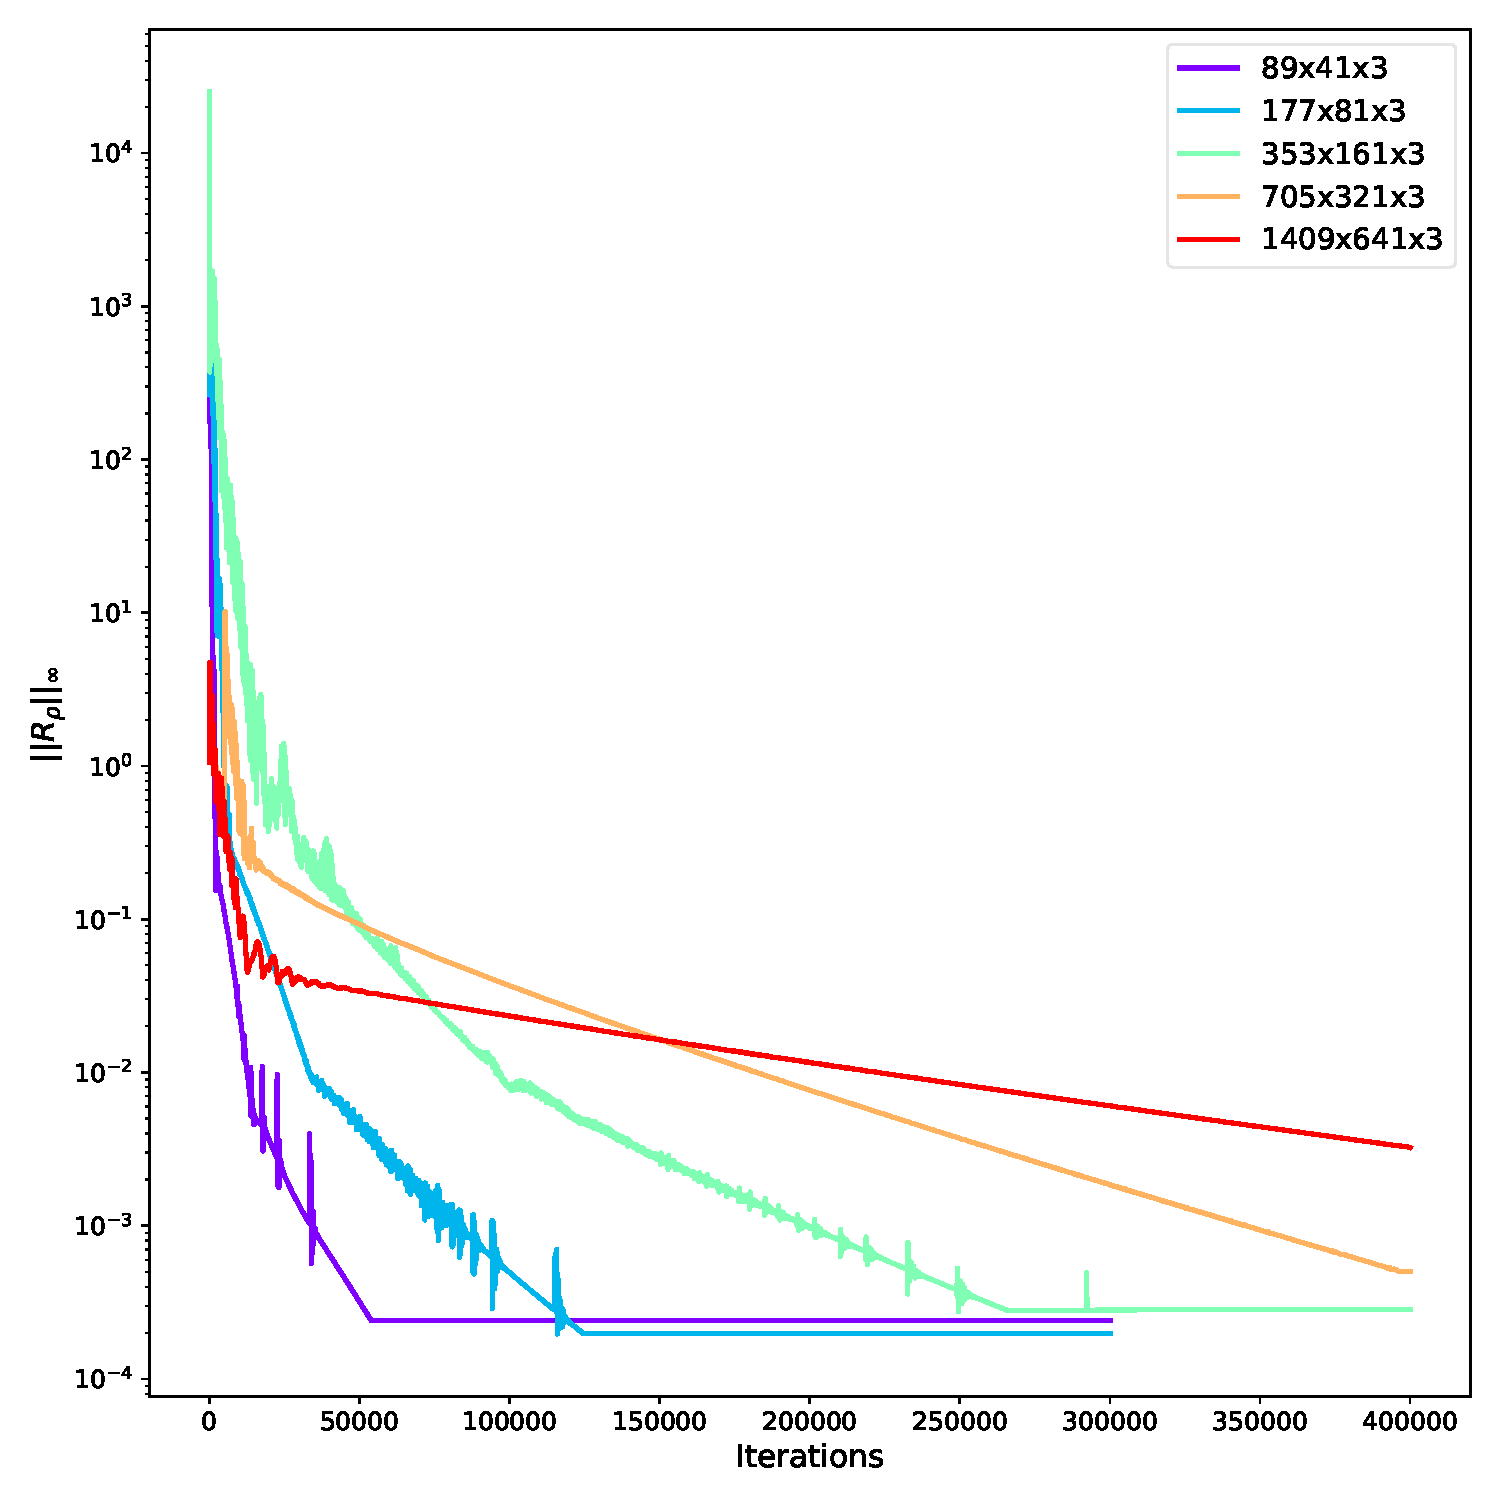
\includegraphics[width=1.0\textwidth]{figs/2dbump/convergenceRho.pdf}
  %\caption{Maximum density residual}
\end{subfigure}%
%\begin{subfigure}{.45\textwidth}
%  \centering
%  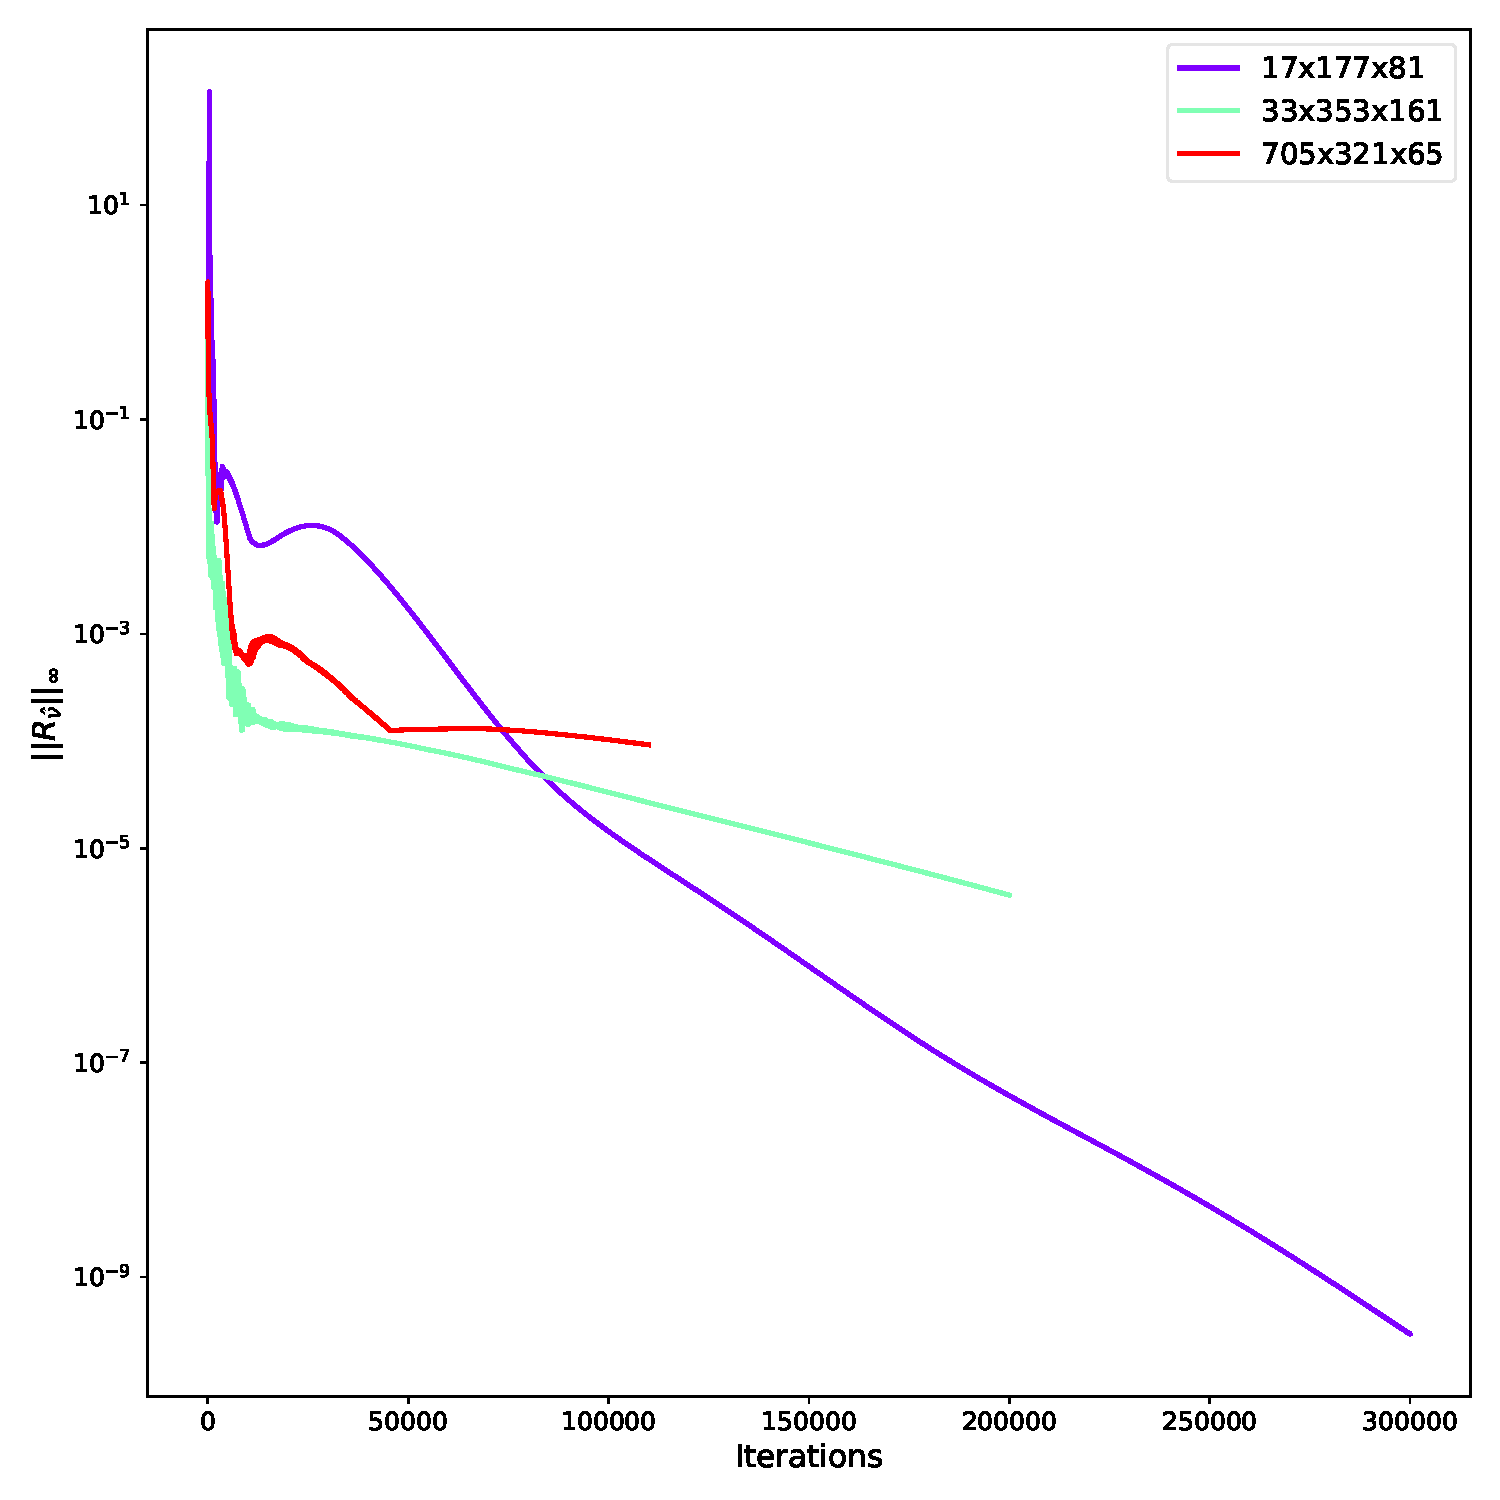
\includegraphics[width=1.0\textwidth]{figs/2dbump/convergencesa.pdf}
%  \caption{Maximum turbulence variable residual.}
%\end{subfigure}
\caption{2D Bump (syn3D): Convergence of maximum density residual on various grid sizes.}
\label{fig:syn2dbumpcnvstudy}
\end{figure}

\begin{figure}[ht!]
\centering
	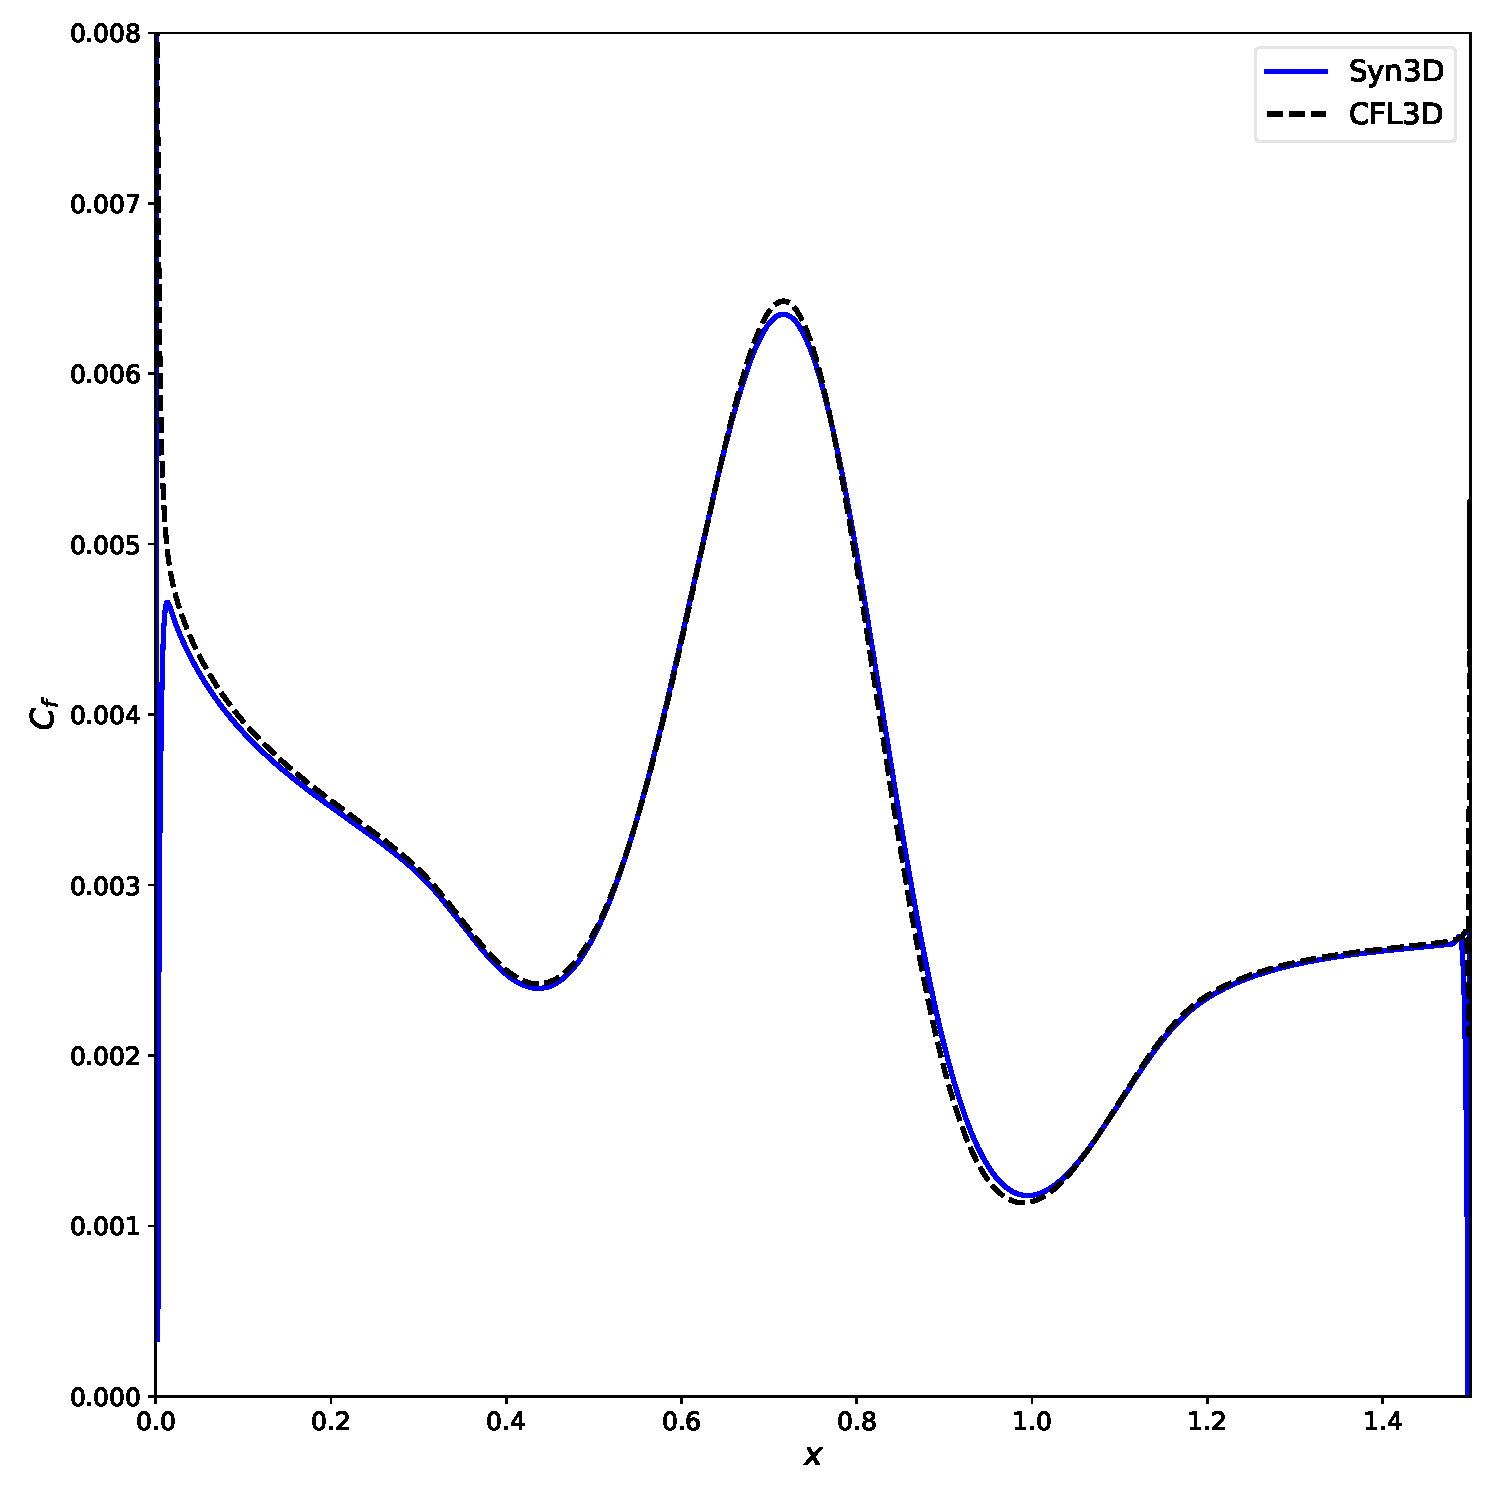
\includegraphics[width=0.7\textwidth]{figs/2dbump/CoefficientFriction.pdf}
    \caption{2D Bump (syn3D): Coefficient of skin friction distribution along the bump.}
    \label{fig:syn2dbumpcf}
\end{figure}


\begin{figure}[ht!]
\centering
	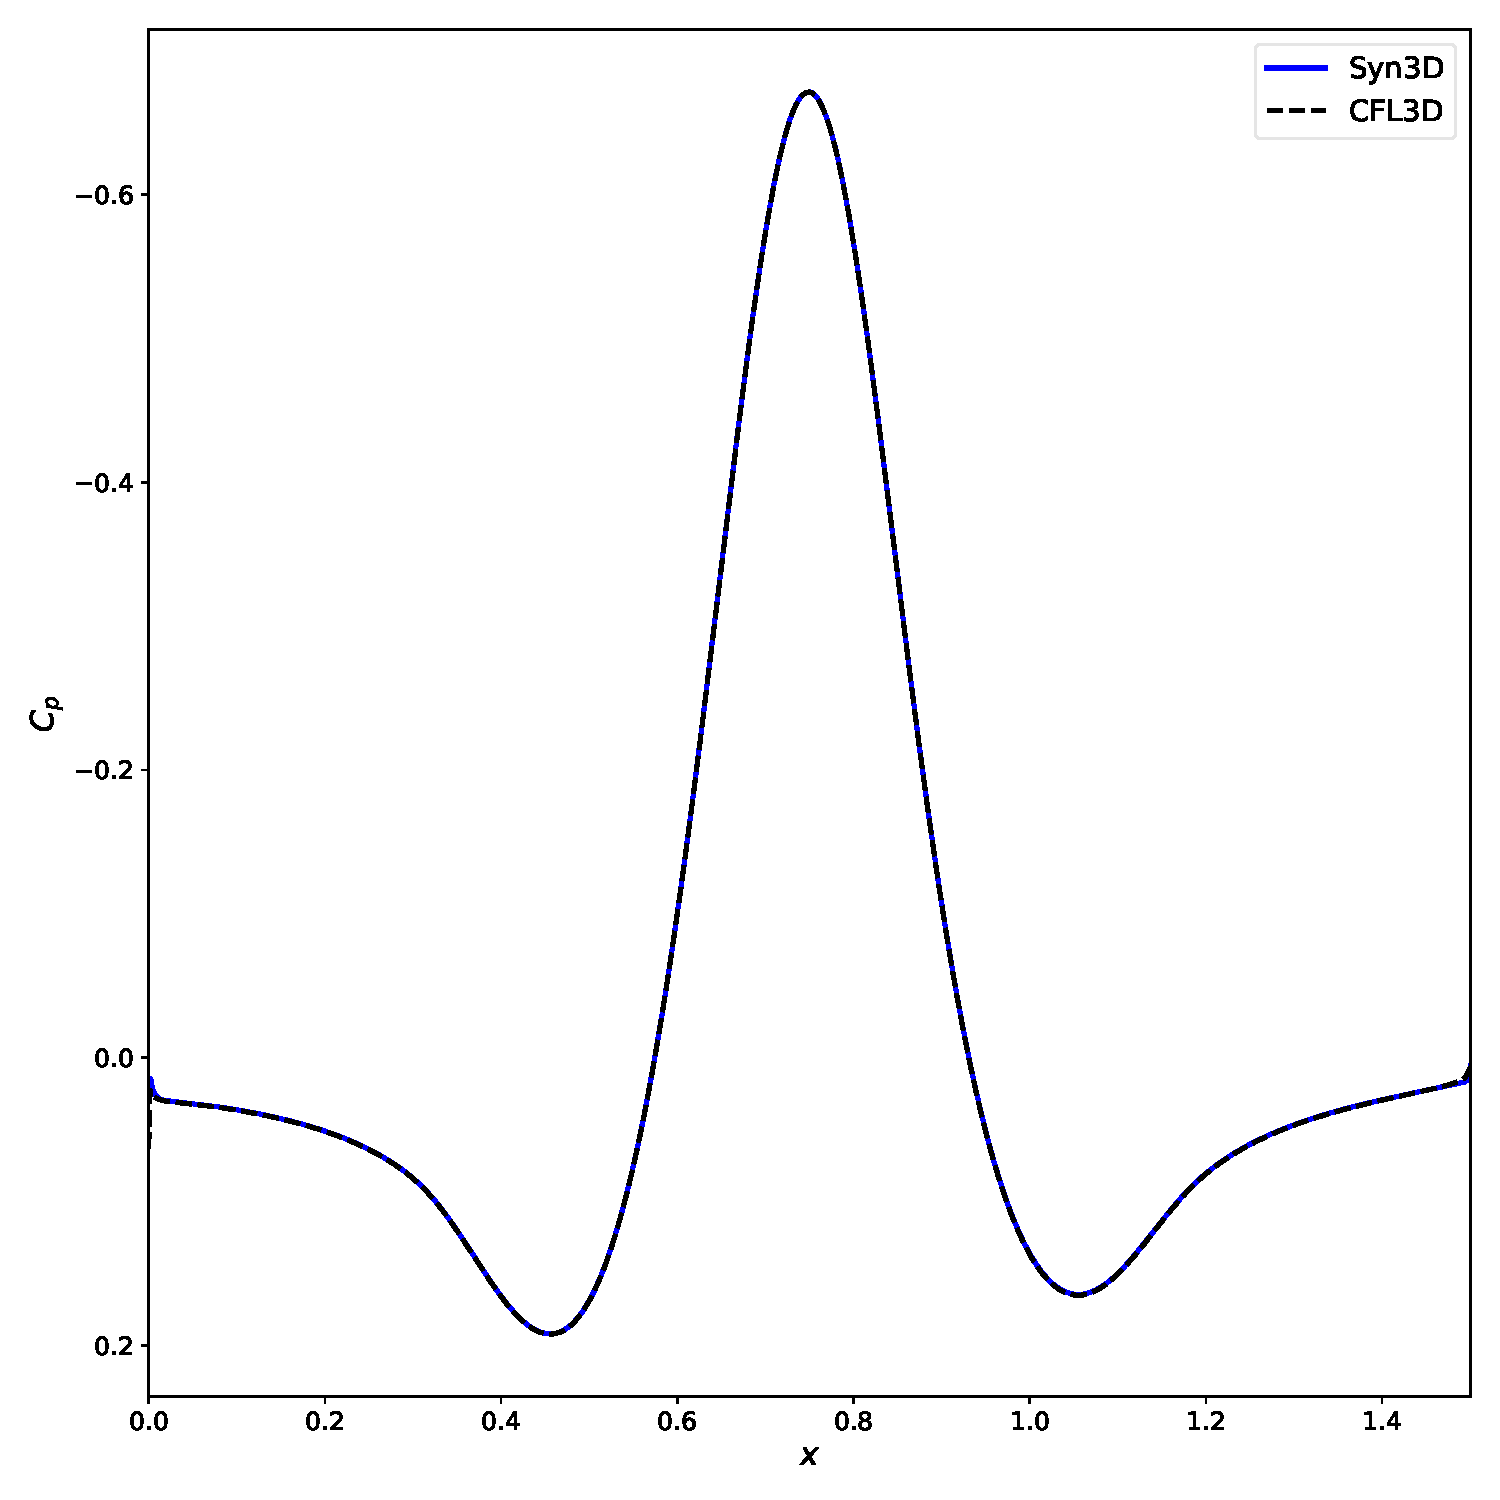
\includegraphics[width=0.7\textwidth]{figs/2dbump/CoefficientPressure.pdf}
    \caption{2D Bump (syn3D): Coefficient of pressure distribution along the bump.}
    \label{fig:syn2dbumpcp}
\end{figure}


\begin{figure}[ht!]
\centering
\begin{subfigure}{.45\textwidth}
  \centering
  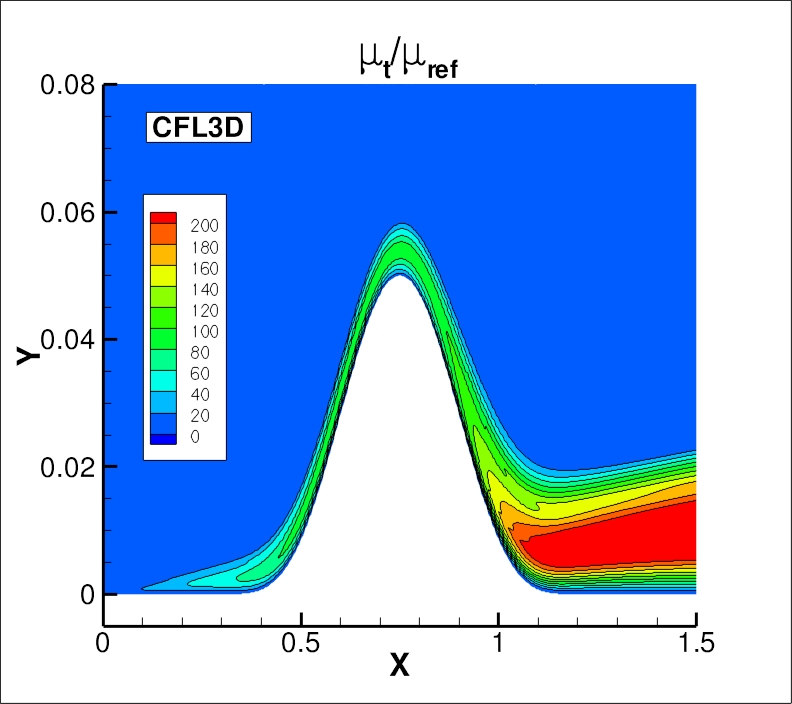
\includegraphics[width=1.0\textwidth]{figs/2dbump/MutNASA.jpg}
  \caption{CFL3D}
\end{subfigure}%
\begin{subfigure}{.45\textwidth}
  \centering
  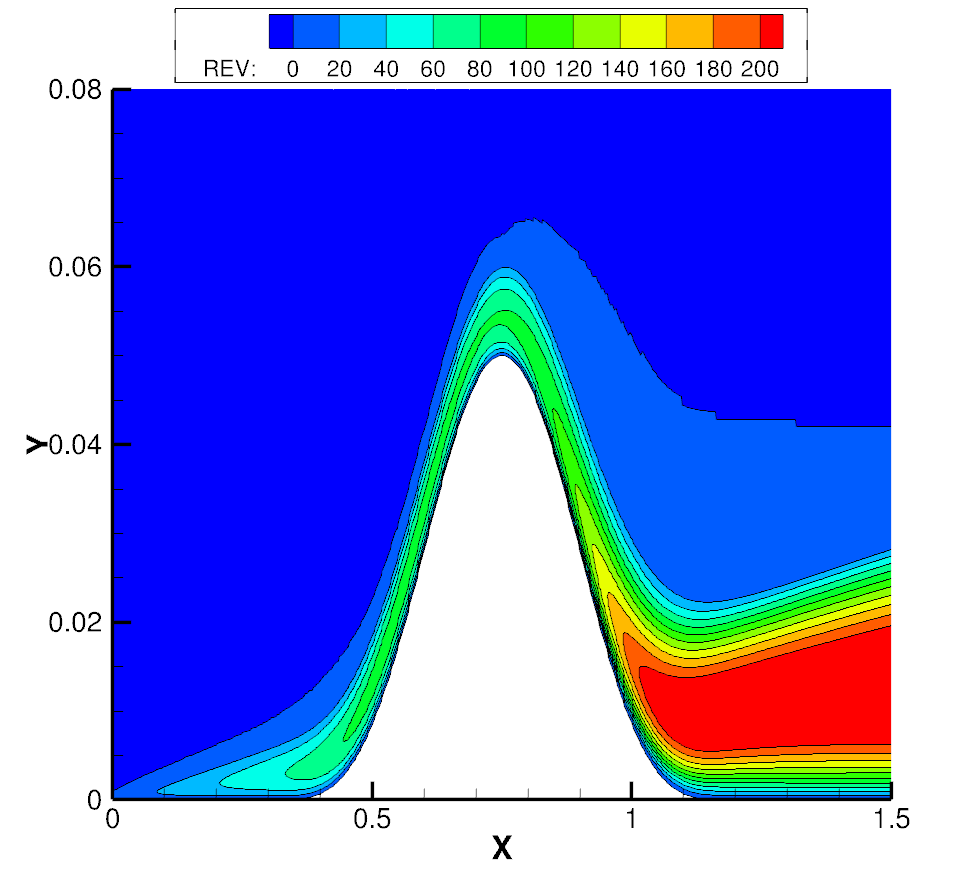
\includegraphics[width=1.0\textwidth]{figs/2dbump/RevContour2.png}
  \caption{syn3D}
\end{subfigure}
\caption{2D Bump (syn3D): Contours of $\mu_T/\mu_{\infty}$.}
\label{fig:syn2dbumpmutcontour}
\end{figure}

\begin{figure}[ht!]
\centering
\begin{subfigure}{.45\textwidth}
  \centering
  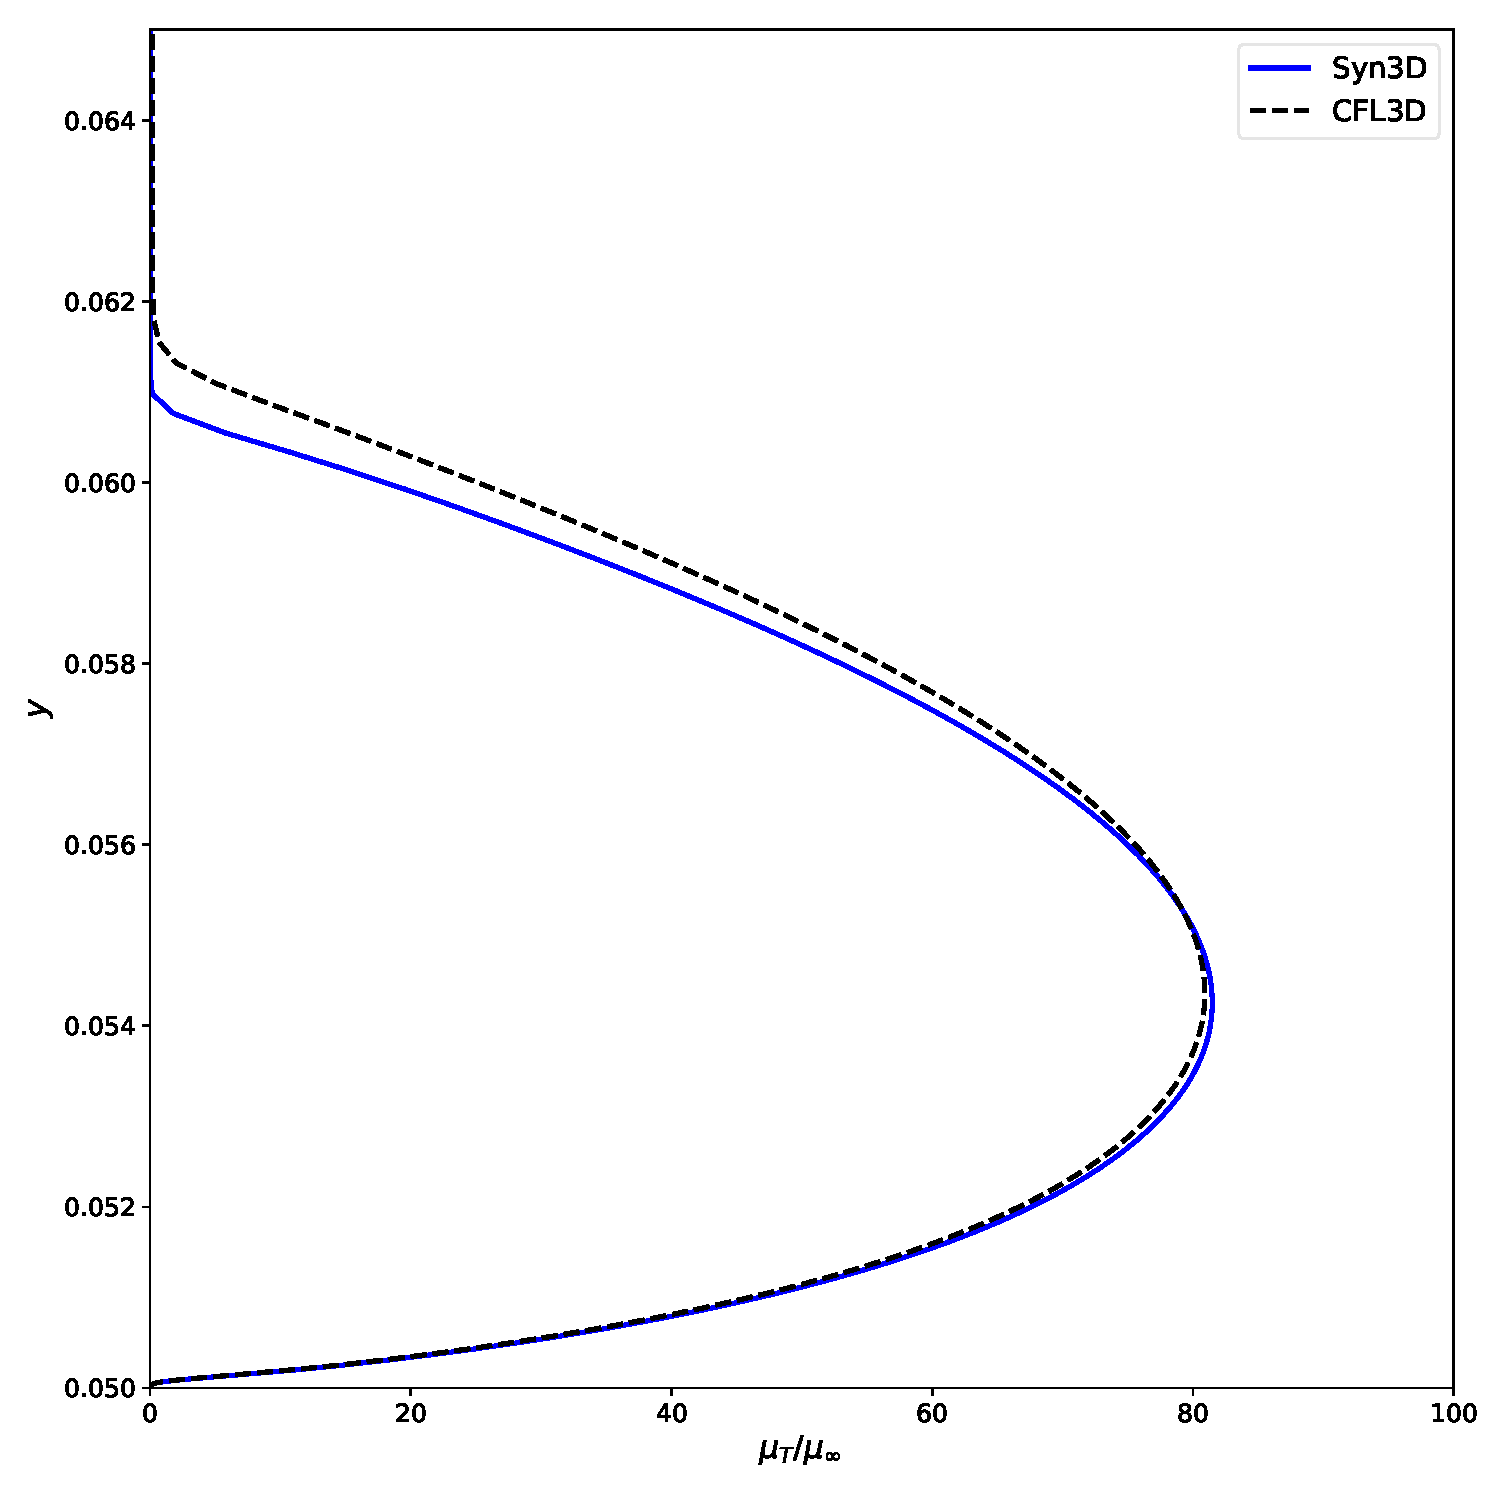
\includegraphics[width=1.0\textwidth]{figs/2dbump/revBL.pdf}
  \caption{Profile at $x=0.75$}
  \label{fig:syn2dbumpmutprof}
\end{subfigure}%
\begin{subfigure}{.45\textwidth}
  \centering
  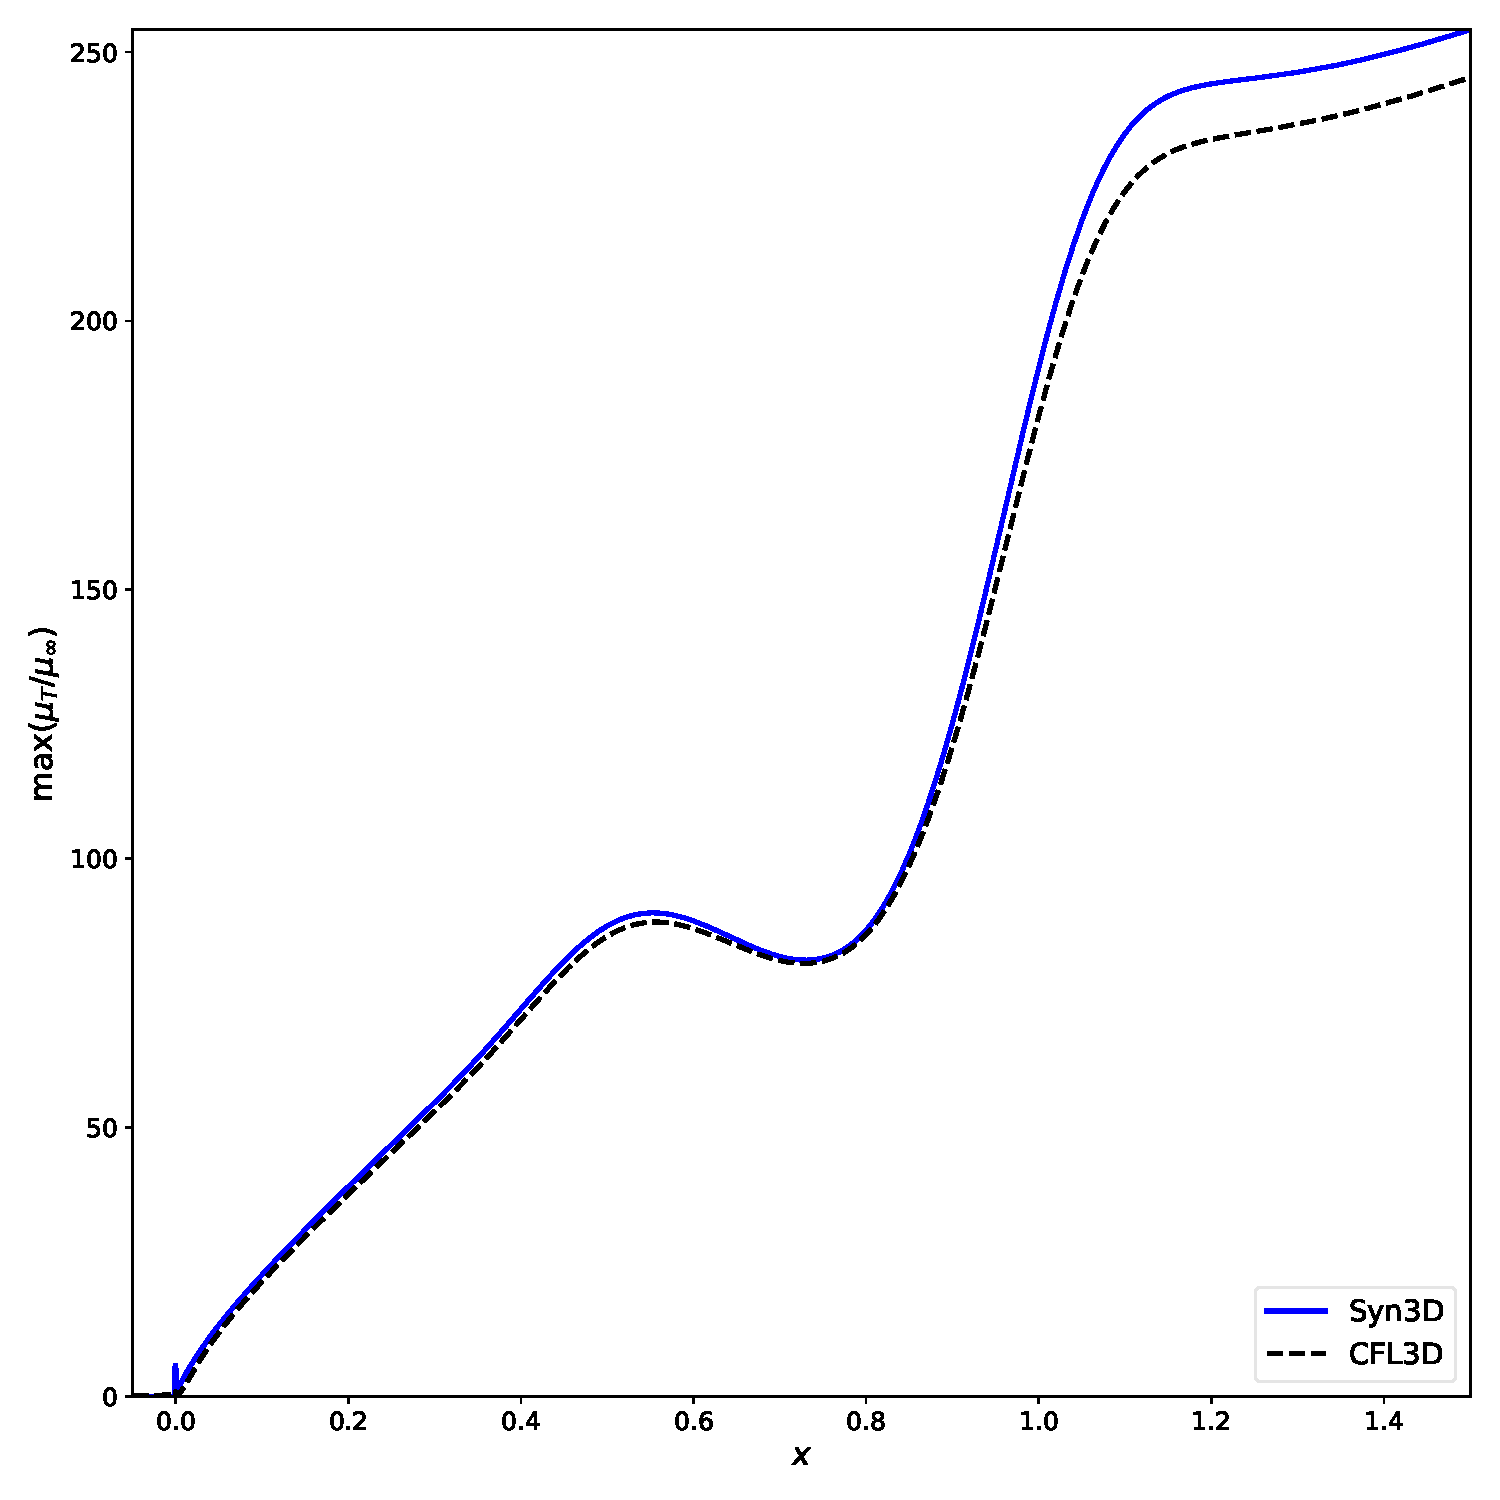
\includegraphics[width=1.0\textwidth]{figs/2dbump/maxRev.pdf}
  \caption{Maximum value in the boundary layer.}
  \label{fig:syn2dbumpmaxmut}
\end{subfigure}
\caption{2D Bump (syn3D): Dimensionless eddy viscosity profiles.}
\label{fig:syn2dbumpmut}
\end{figure}

\begin{figure}[ht!]
\centering
\begin{subfigure}{.45\textwidth}
  \centering
  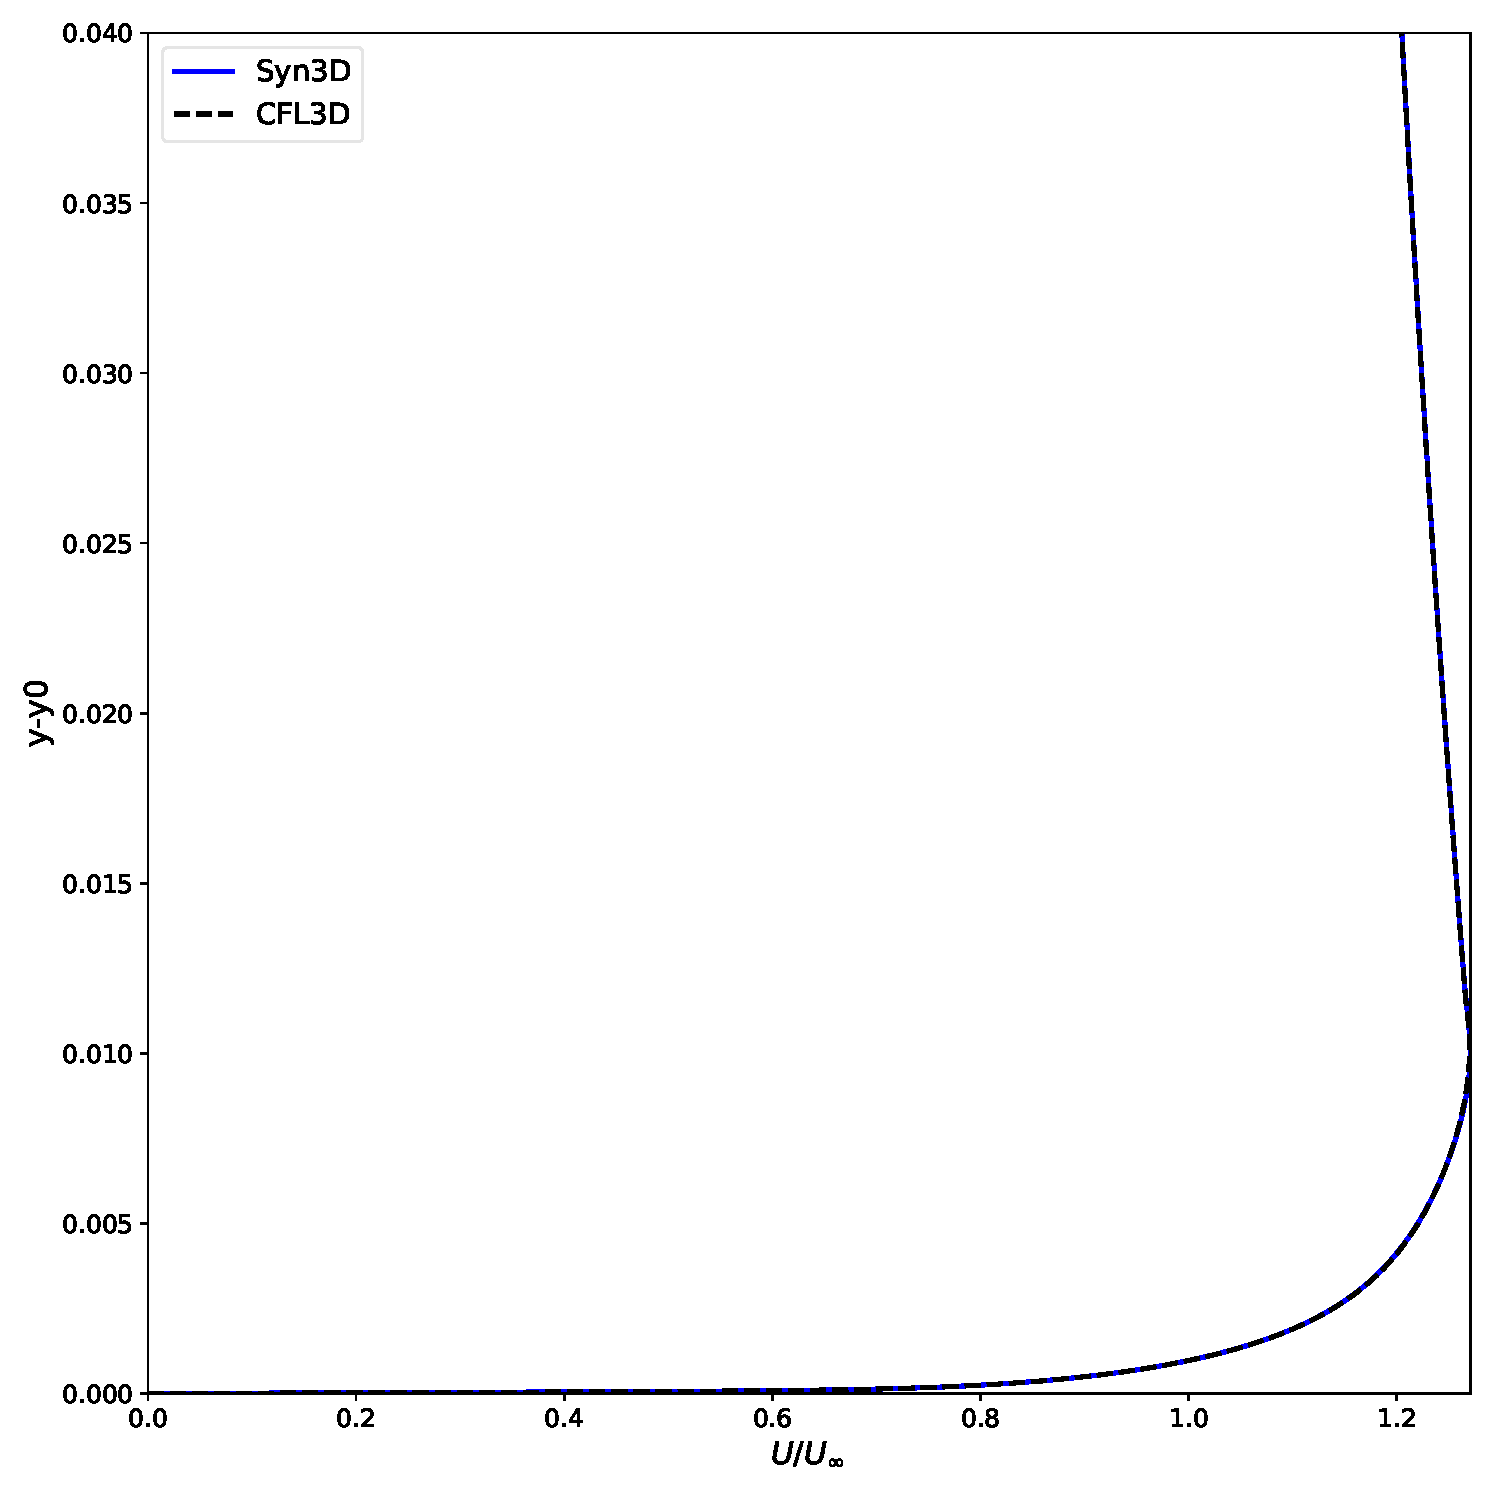
\includegraphics[width=1.0\textwidth]{figs/2dbump/u75.pdf}
  \caption{$x=0.75$}
\end{subfigure}%
\begin{subfigure}{.45\textwidth}
  \centering
  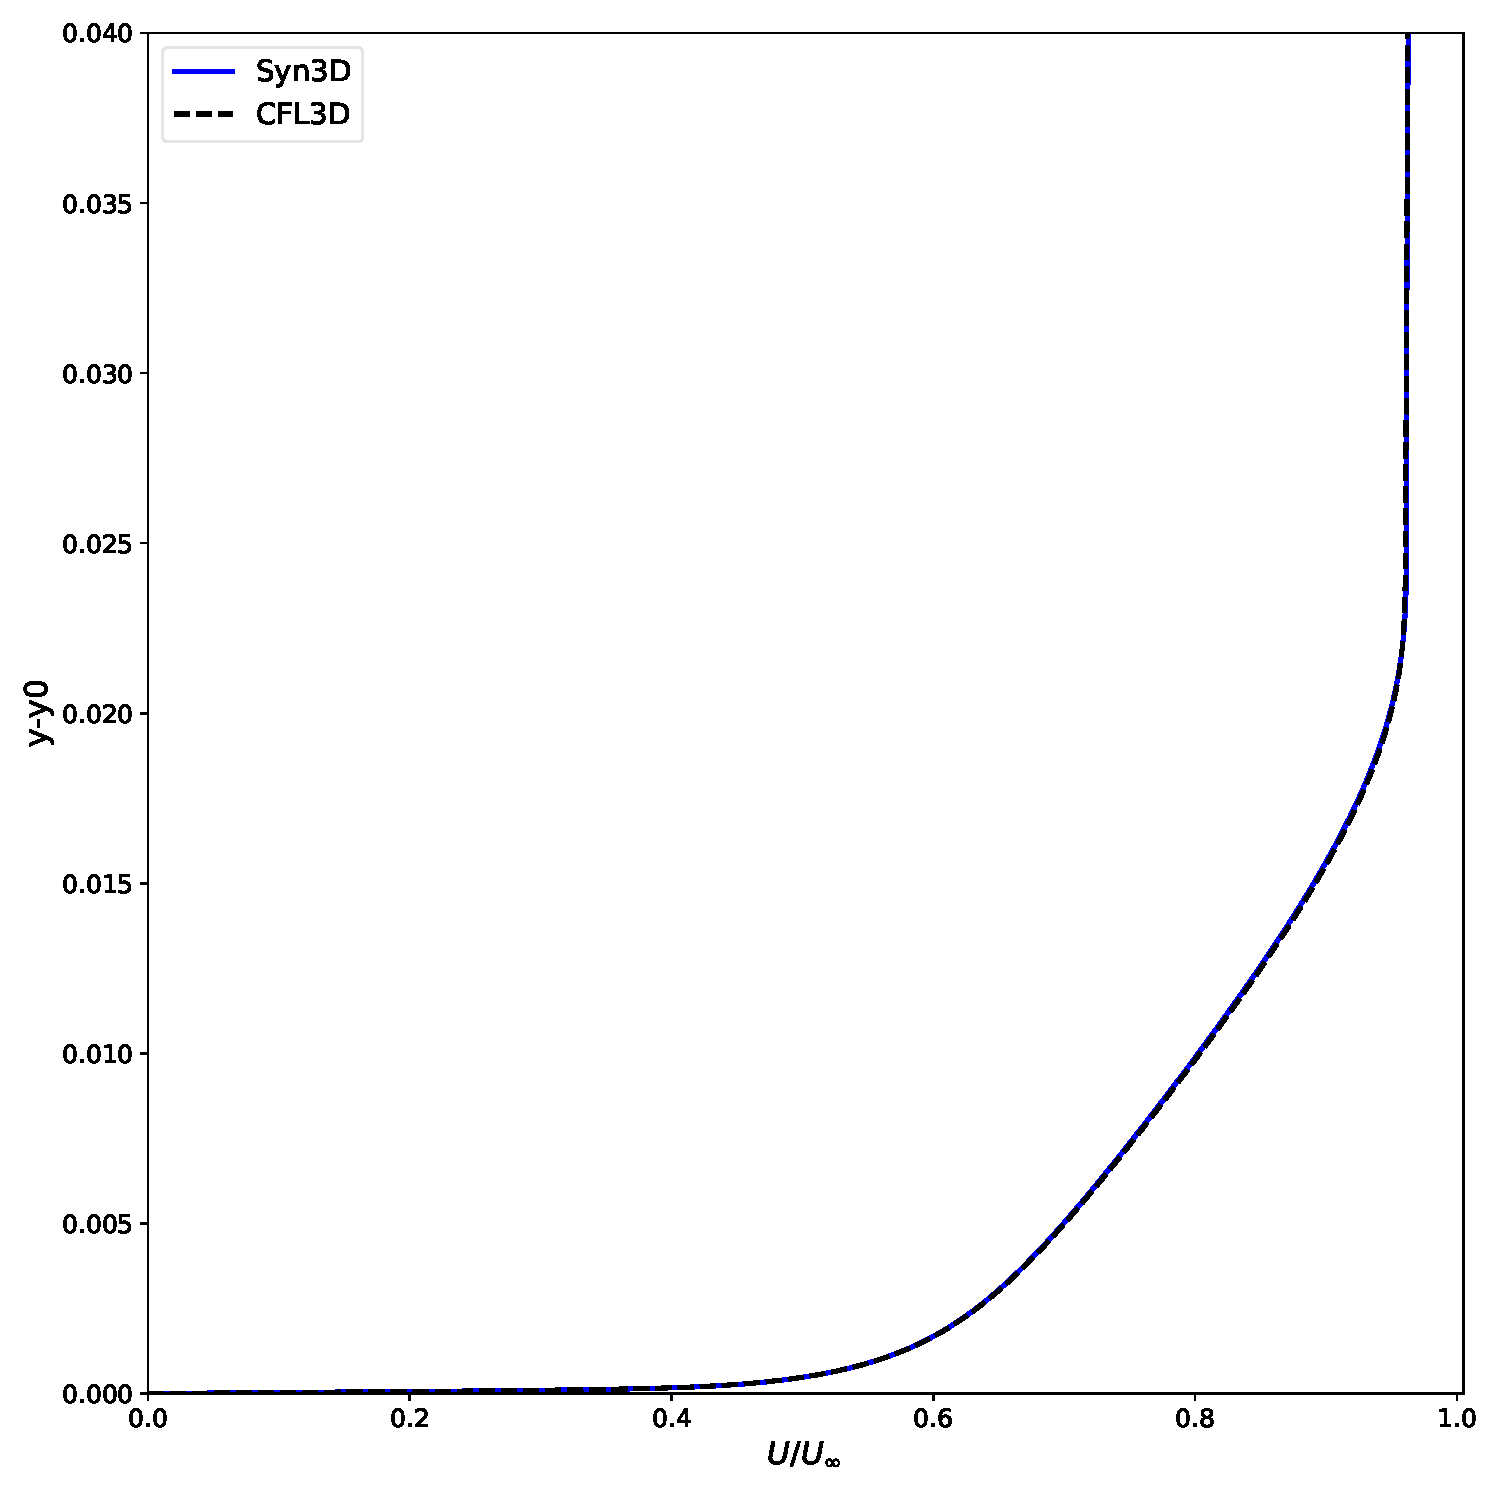
\includegraphics[width=1.0\textwidth]{figs/2dbump/u120148.pdf}
  \caption{$x=1.20148$}
\end{subfigure}
\caption{2D Bump (syn3D): Dimensionless velocity profiles $U/U_\infty$.}
\label{fig:syn2dbumpu}
\end{figure}

\Cref{fig:syn2dbumpcf} compares the $C_f$ distribution over the bump for the finest grid. The skin friction coefficient can be seen to start high, slowly decrease in the flat portion as it did for the flat plate, and then increase on the bump as it accelerates. The value of $C_f$ is under-predicted syn3D until the peak of the bump, after which point it is over-predicted.

\Cref{fig:syn2dbumpcp} shows the $C_p$ distribution. The trend in this plot is similar to the skin friction plot. The pressure decreases as the flow accelerates at the leading edge of the bump. The pressure then increases again once the peak is reached. The pressure coefficient is identical between syn3D and CFL3D, as is the drag force due to the pressure component $C_{Dp}$ (see~\Cref{tab:syn2dbump1}).

\Cref{fig:syn2dbumpmutcontour} compares the contour of eddy viscosity over the bump. Both contour plots show similar trends. However, values of $\mu_t$ in the downstream region are slightly elevated for syn3D.

\Cref{fig:syn2dbumpmut} compares the eddy viscosity through line plots. Similar to the flat plate, $\mu_t$ increases with $x$. Once again, syn3D displays a small peak in eddy viscosity at the leading edge ($x=0.0$). The difference of the maximum $\mu_t$ value between syn3D and CFL3D is, as mentioned previously, greater in the downstream region. In, \Cref{fig:syn2dbumpmutprof}, it can again be seen that the eddy viscosity increases with $y$ until it reaches a maximum value and begins to decrease again as it reaches the far-field region. In the region of increasing $\mu_t$ ($y < 0.054$), syn3D and CFL3D show very similar results. In the decreasing region, however, syn3D displays a greater gradient and under-predicts the distance needed for $\mu_t$ to return to its free-stream value.

\Cref{fig:syn2dbumpu} compares the velocity profile. A sharp velocity gradient near the wall is observed at both locations, although the height of the boundary layer is greater as $x$ increases. Profiles are identical between the two solvers.
\begin{figure}[ht!]
\centering
  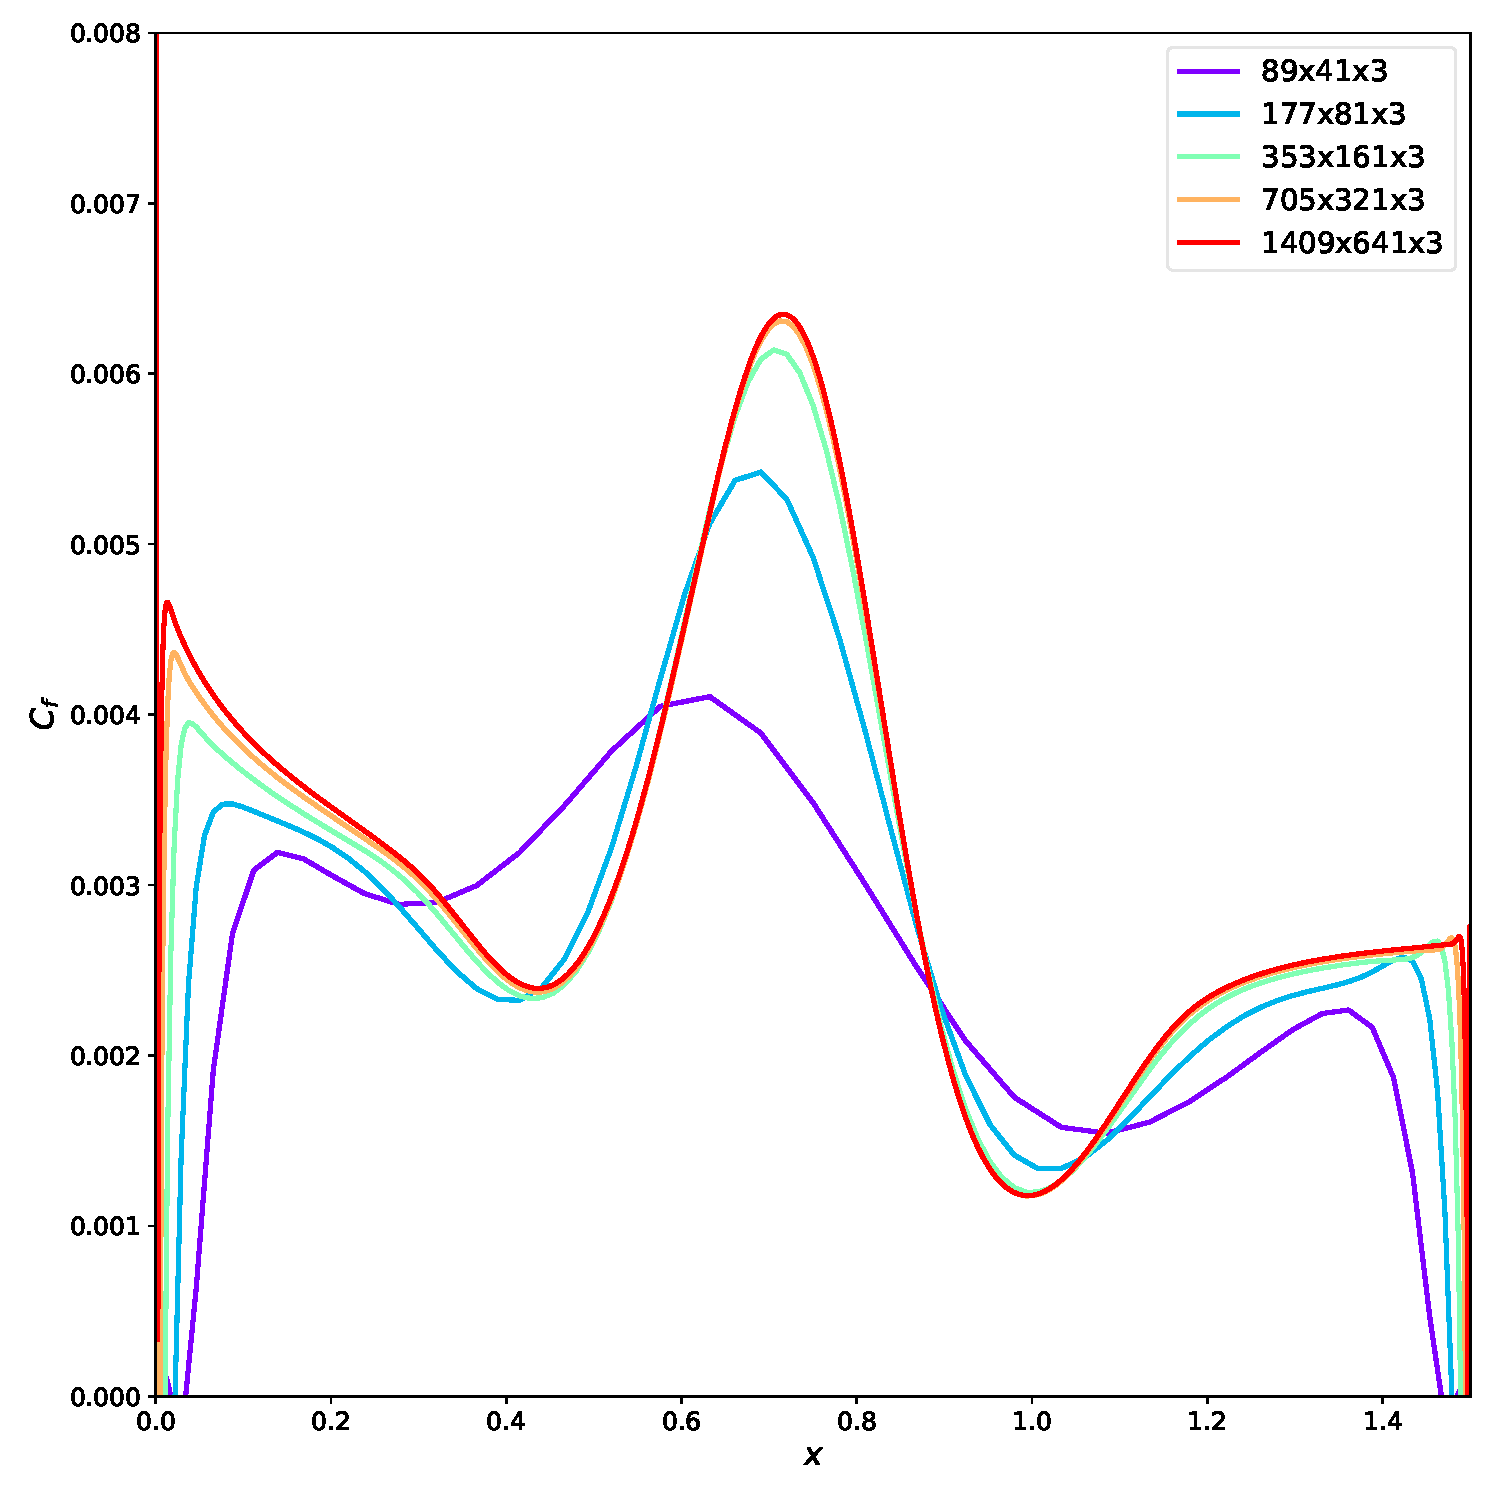
\includegraphics[width=0.7\textwidth]{figs/2dbump/CfGridStudy.pdf}
    \caption{2D Bump (syn3D): Coefficient of skin friction along the bump for various grids.}
    \label{fig:syn2dbumpcfstudy}
\end{figure}

\begin{figure}[ht!]
\centering
  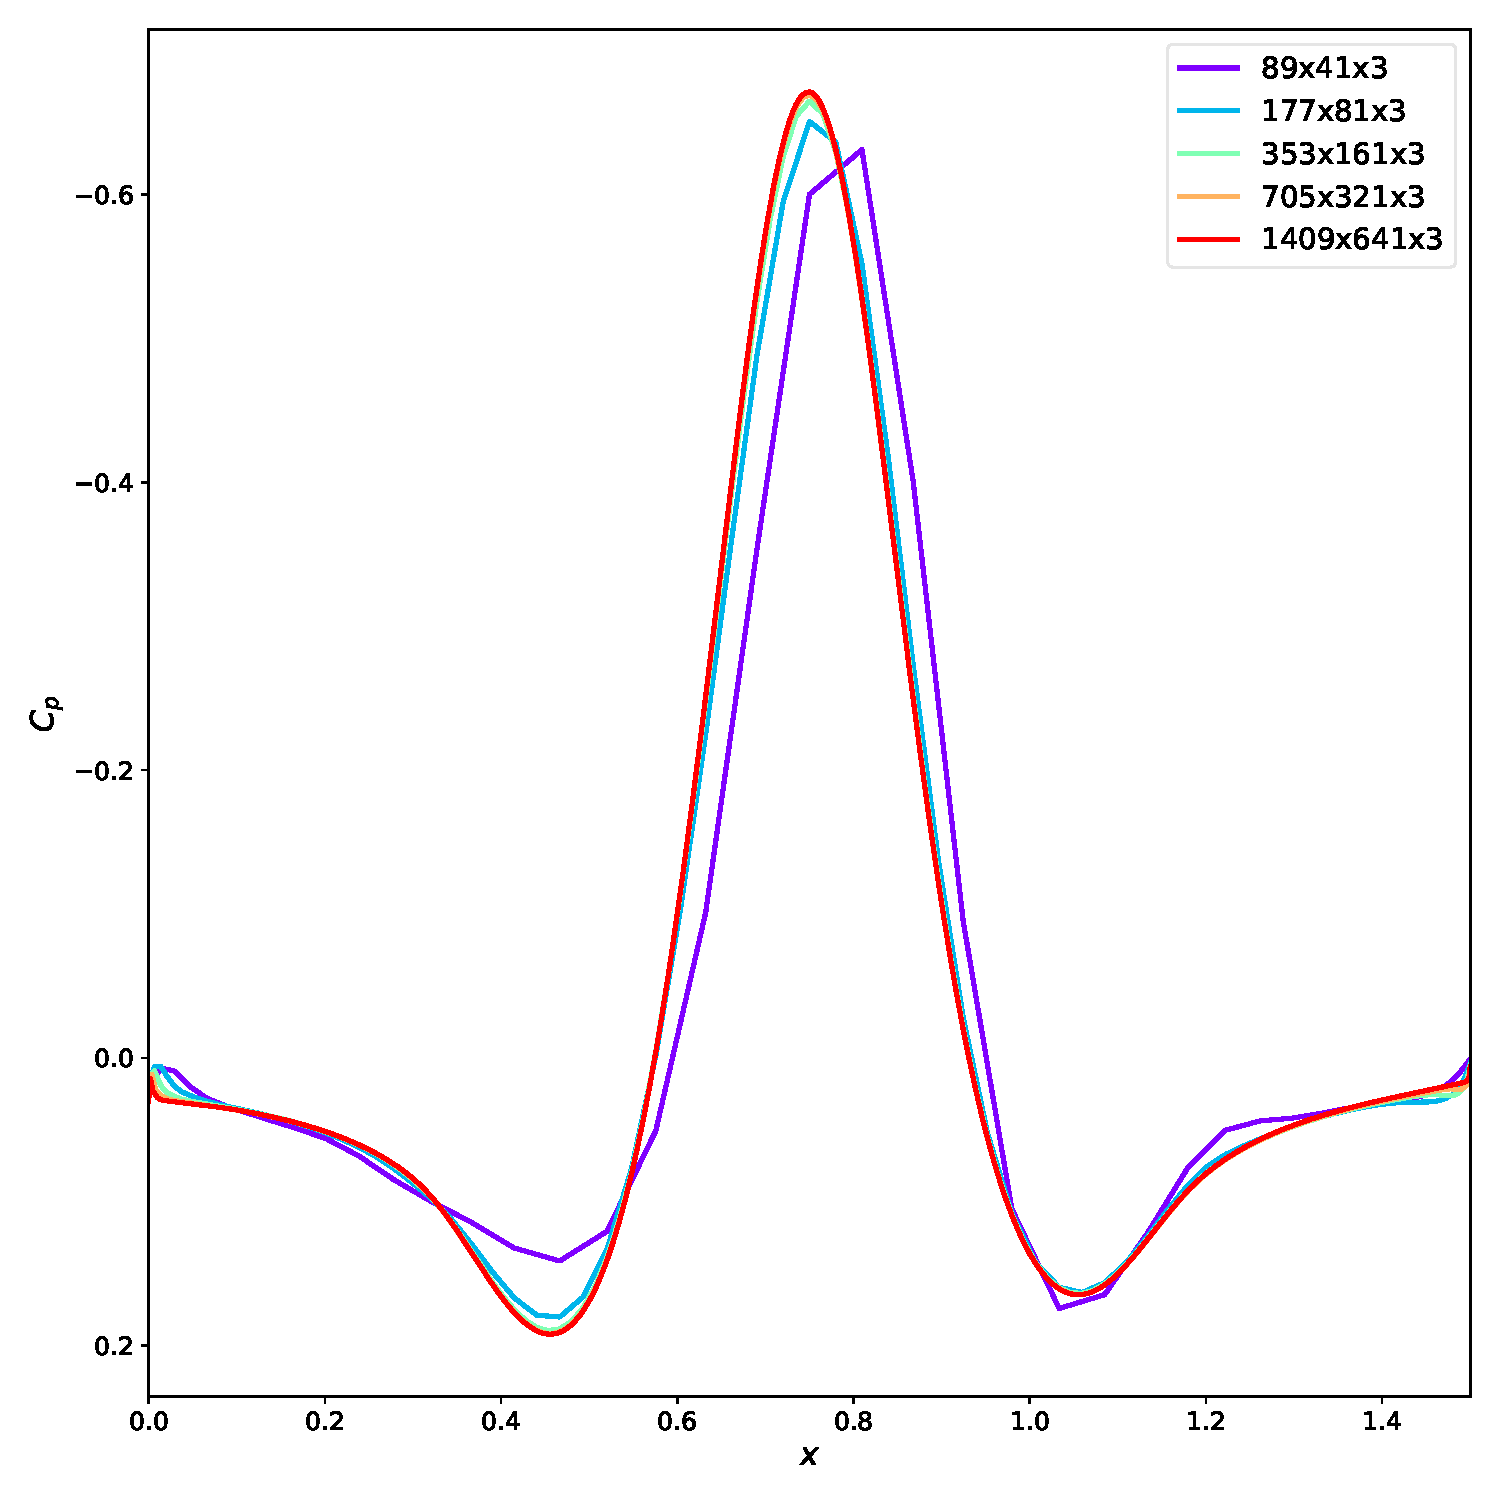
\includegraphics[width=0.7\textwidth]{figs/2dbump/CpGridStudy.pdf}
    \caption{2D Bump (syn3D): Coefficient of pressure along the bump for various grid.}
    \label{fig:syn2dbumpcpstudy}
\end{figure}

\begin{figure}[ht!]
\centering
\begin{subfigure}{.45\textwidth}
  \centering
  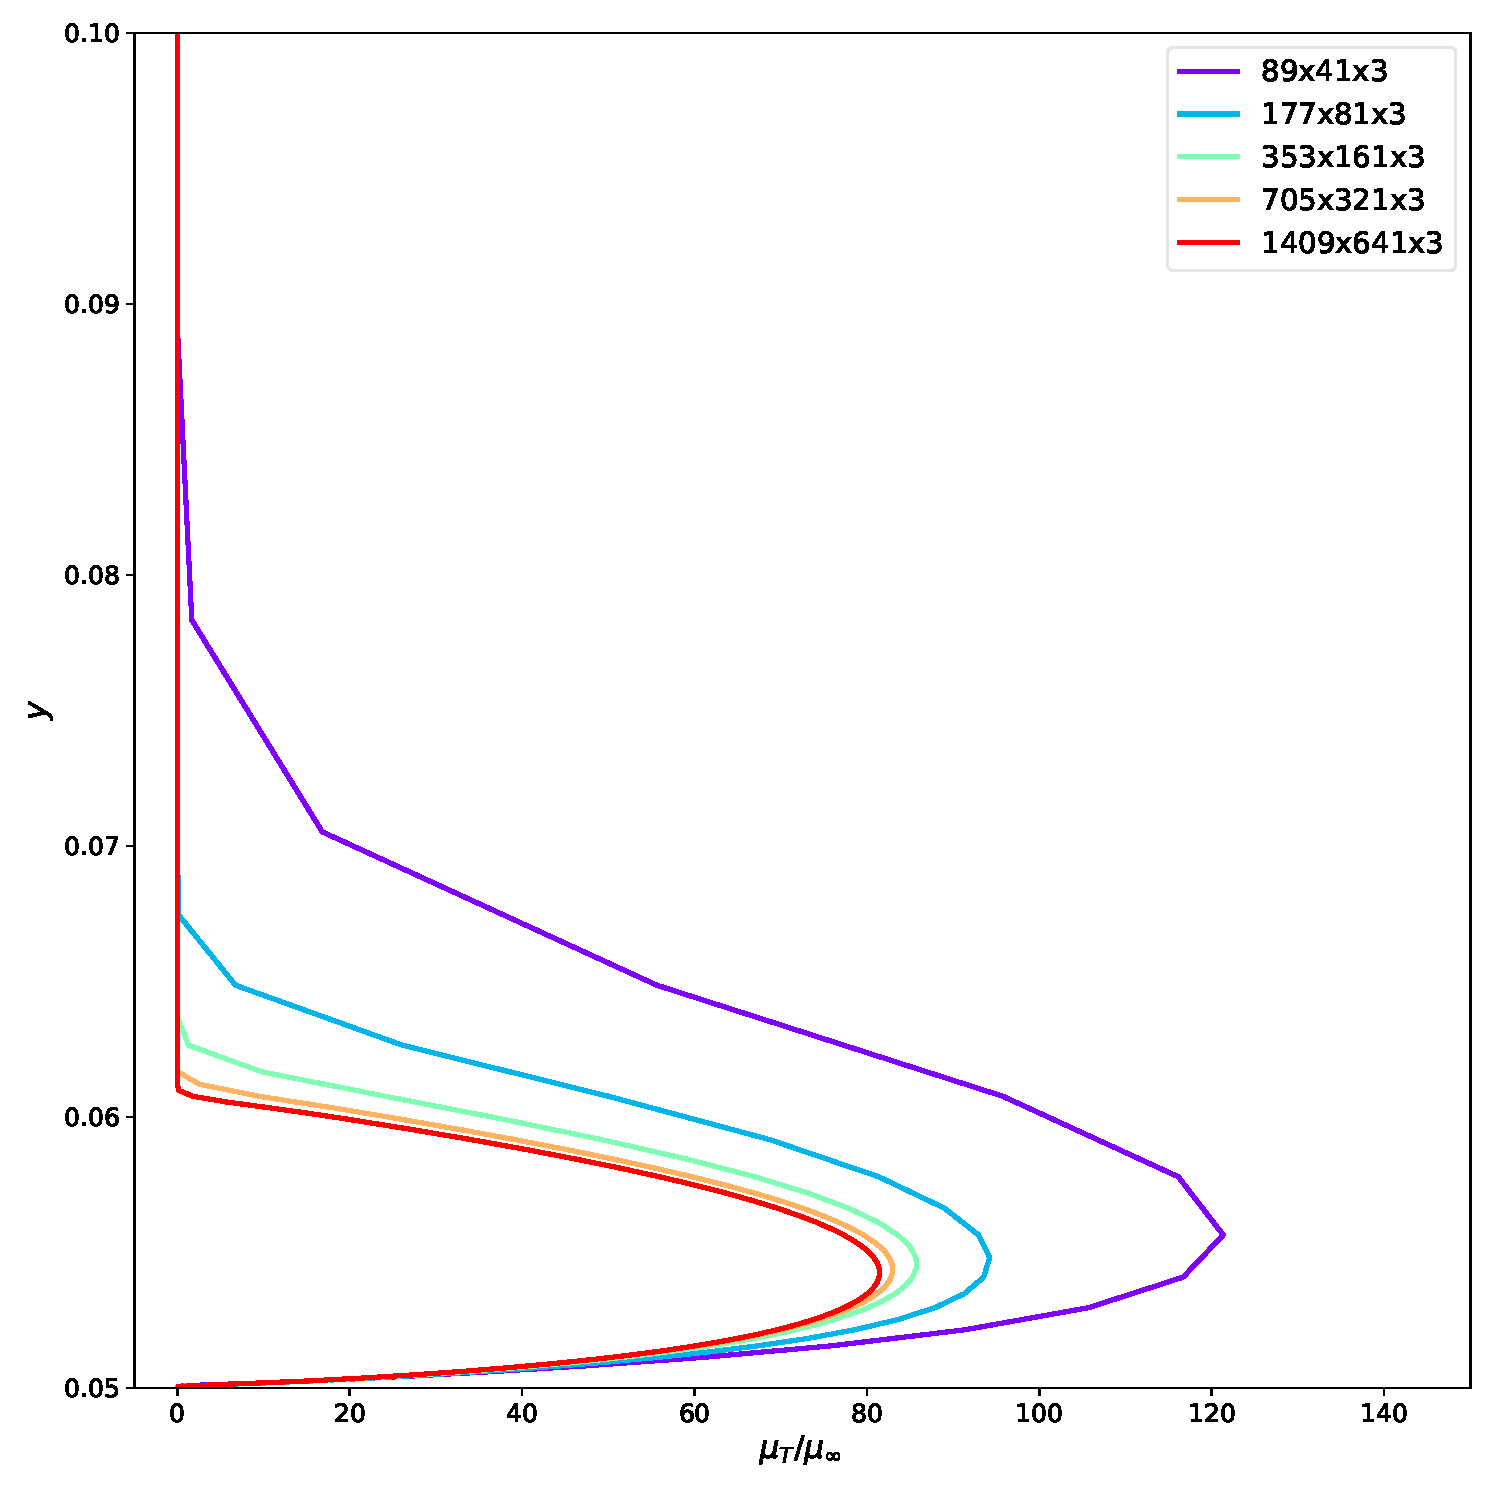
\includegraphics[width=1.0\textwidth]{figs/2dbump/revBLGridStudy.pdf}
  \caption{Profile at $x=0.75$.}
\end{subfigure}%
\begin{subfigure}{.45\textwidth}
  \centering
  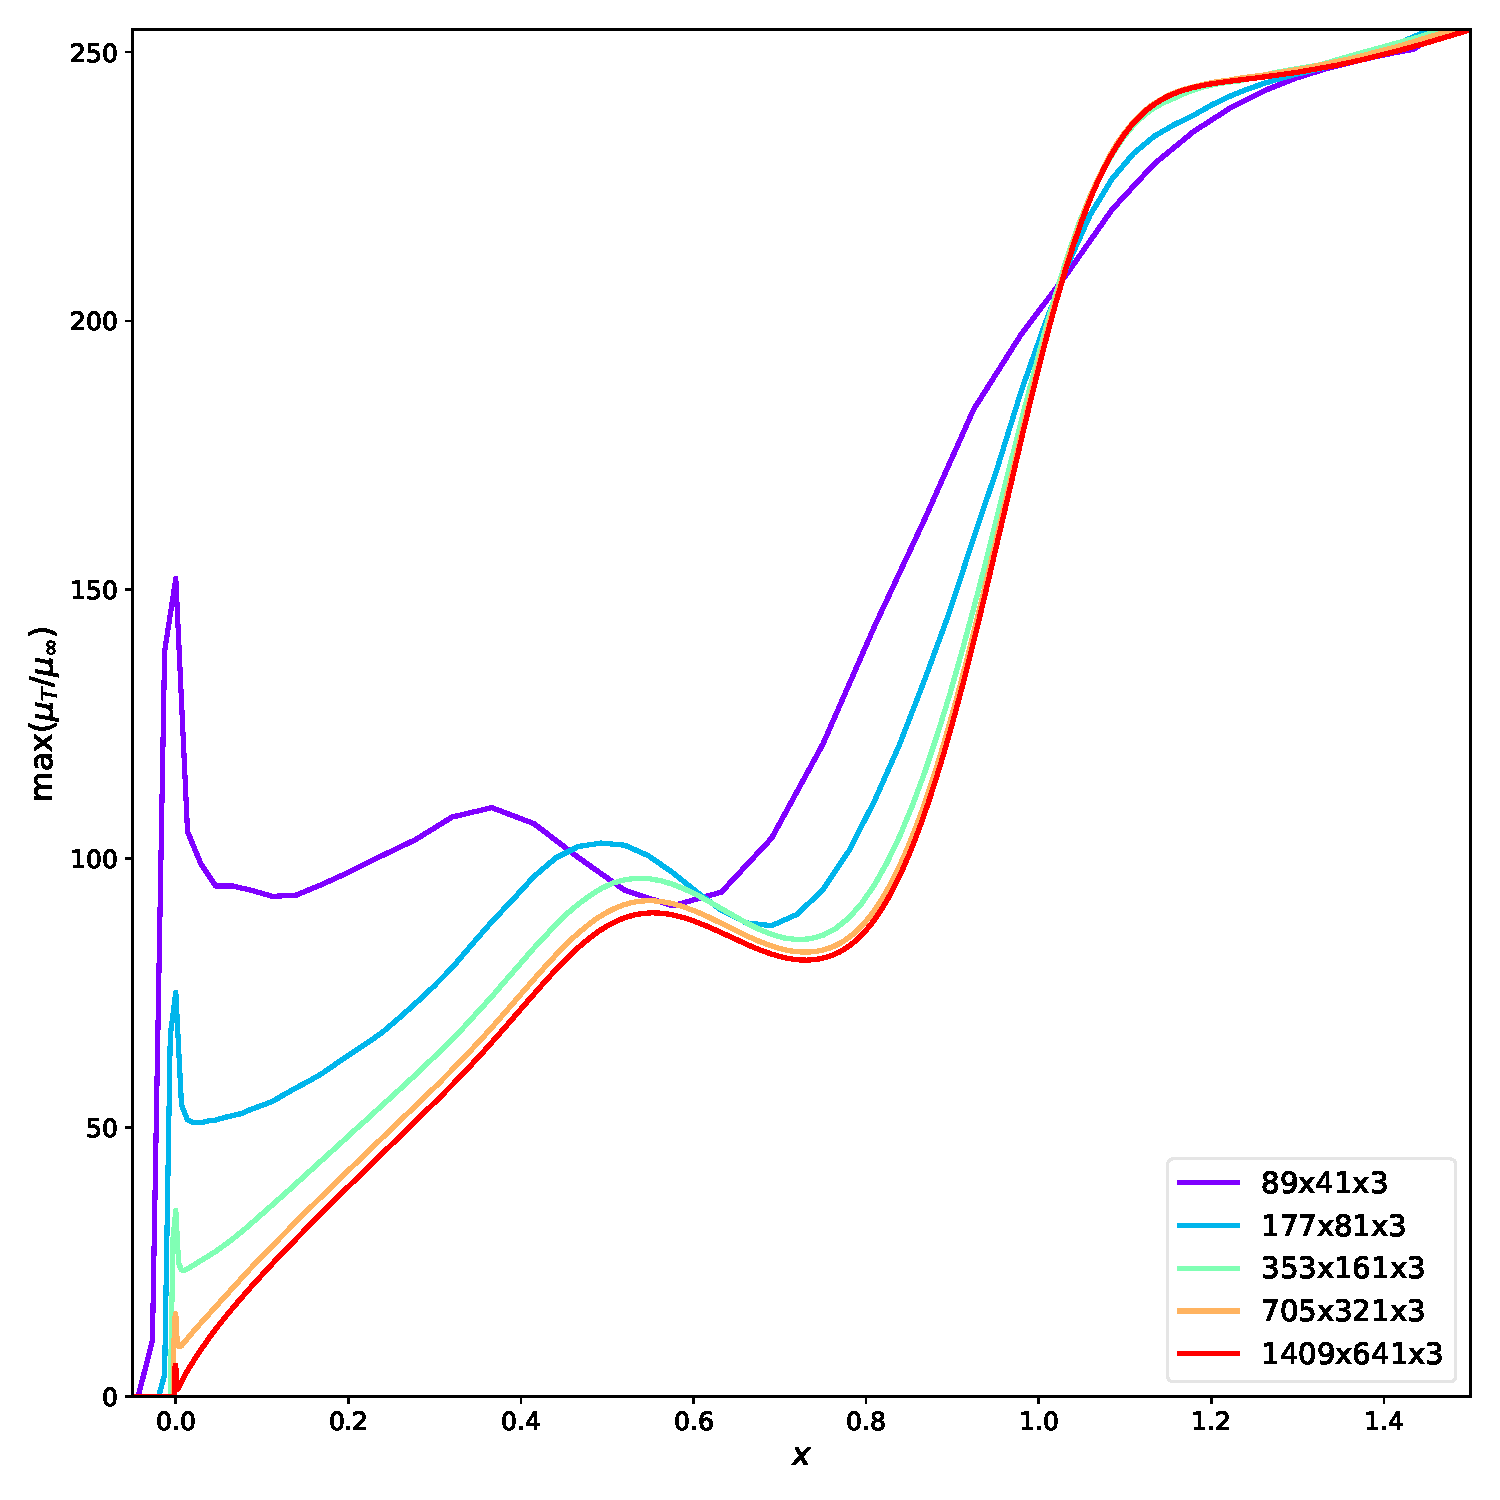
\includegraphics[width=1.0\textwidth]{figs/2dbump/maxRevstudy.pdf}
  \caption{Maximum value in the boundary layer.}
\end{subfigure}
\caption{2D Bump (syn3D): Dimensionless eddy viscosity profiles on the bump for various grids.}
\label{fig:syn2dbumpmutstudy}
\end{figure}

\begin{figure}[ht!]
\centering
\begin{subfigure}{.45\textwidth}
  \centering
  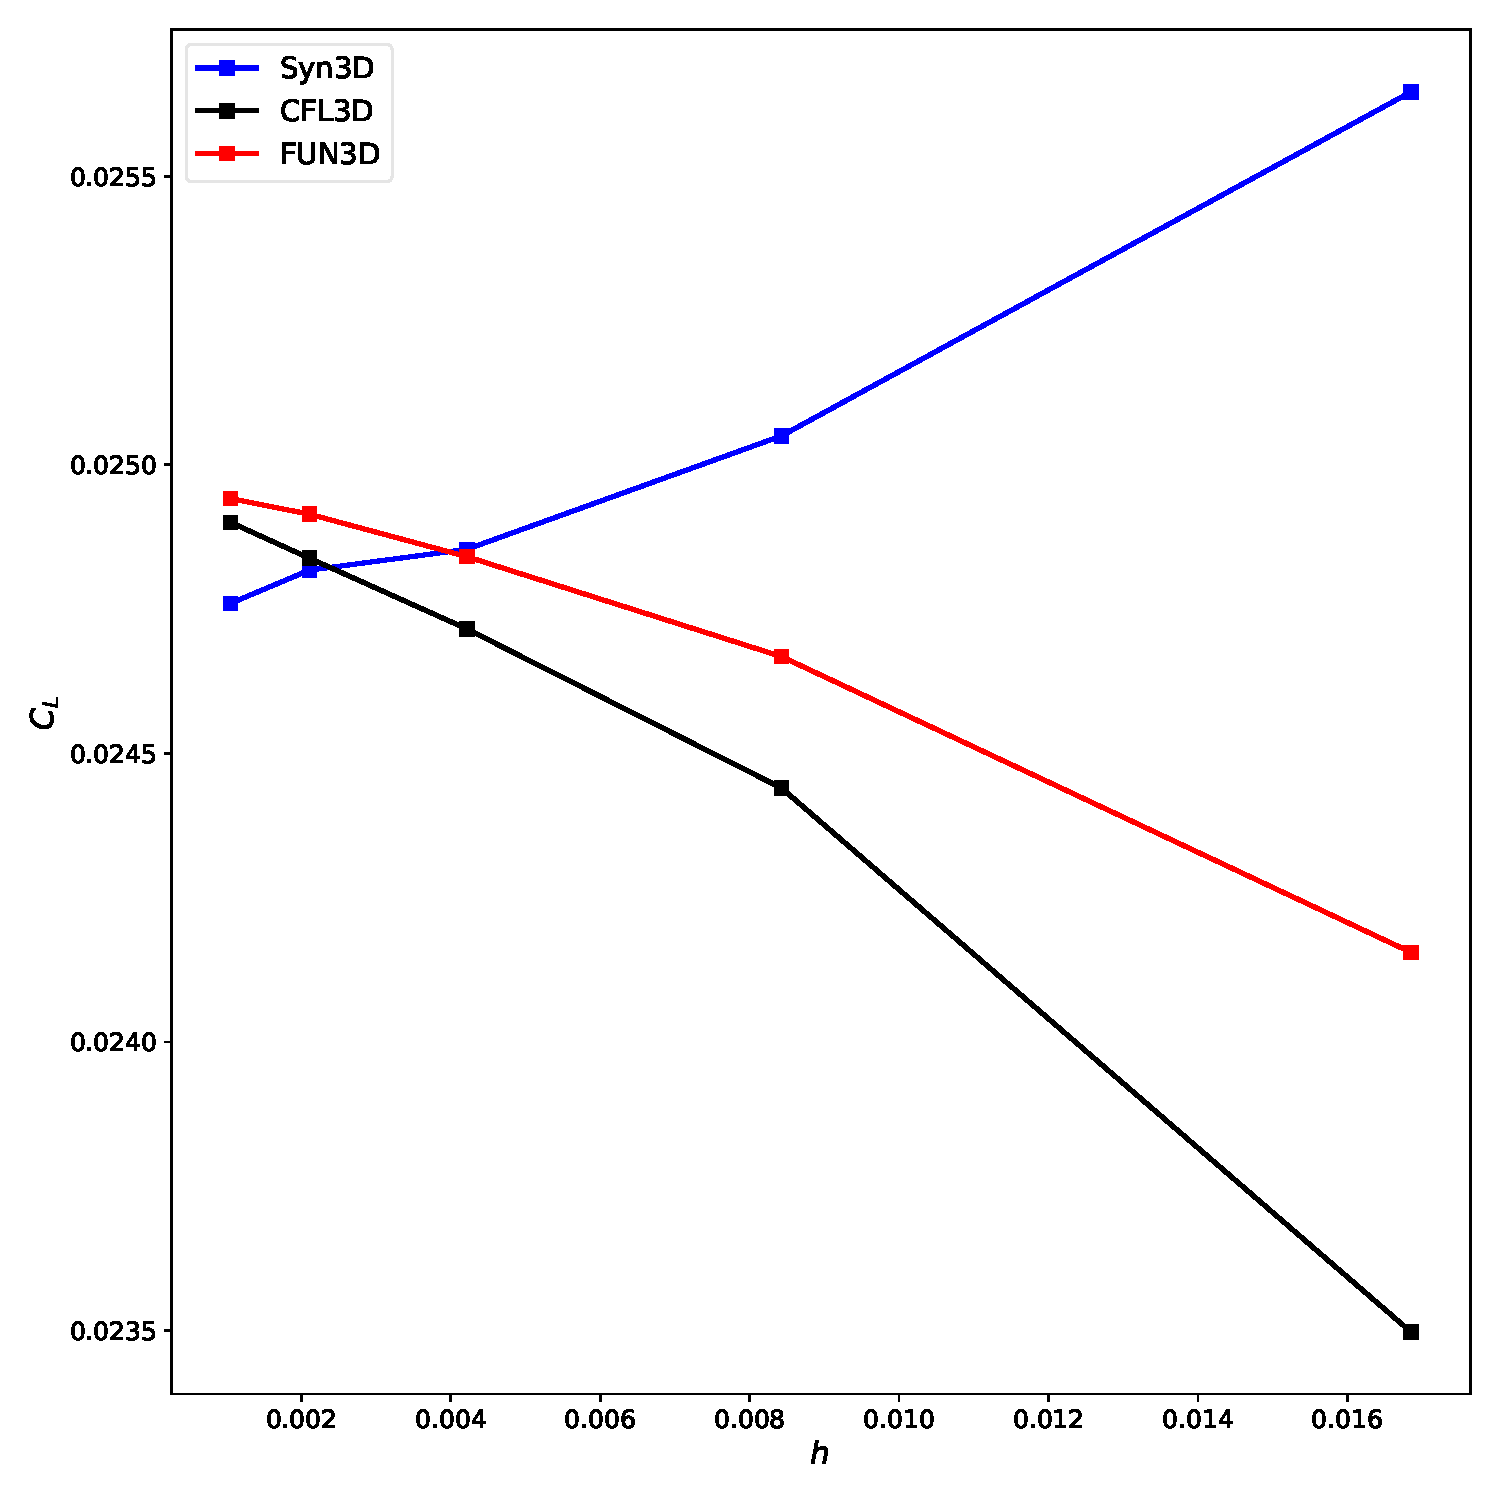
\includegraphics[width=1.0\textwidth]{figs/2dbump/C_LGridStudy.pdf}
  \caption{Lift coefficient.}
\end{subfigure}%
\begin{subfigure}{.45\textwidth}
  \centering
  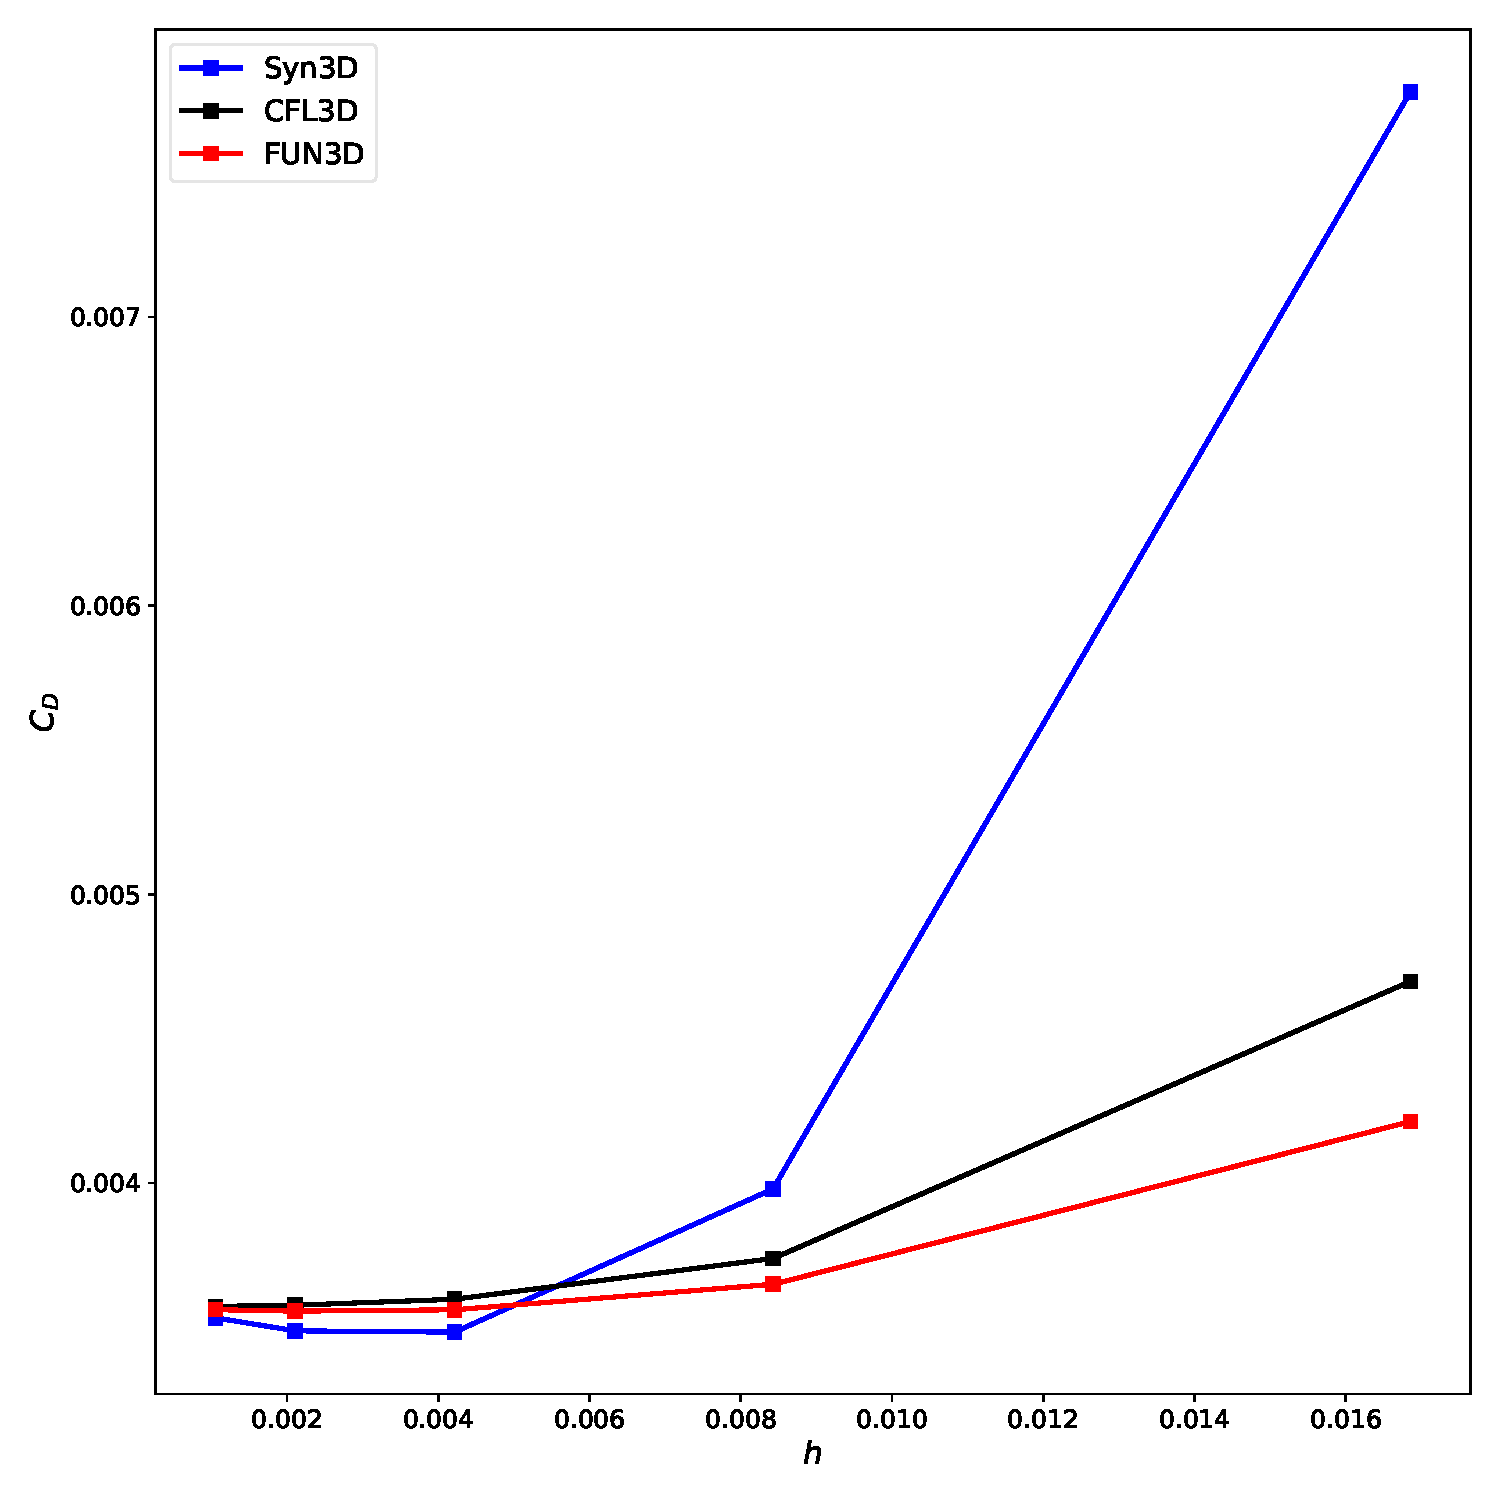
\includegraphics[width=1.0\textwidth]{figs/2dbump/C_DGridStudy.pdf}
  \caption{Drag coefficient.}
\end{subfigure}
\\
\begin{subfigure}{.45\textwidth}
  \centering
  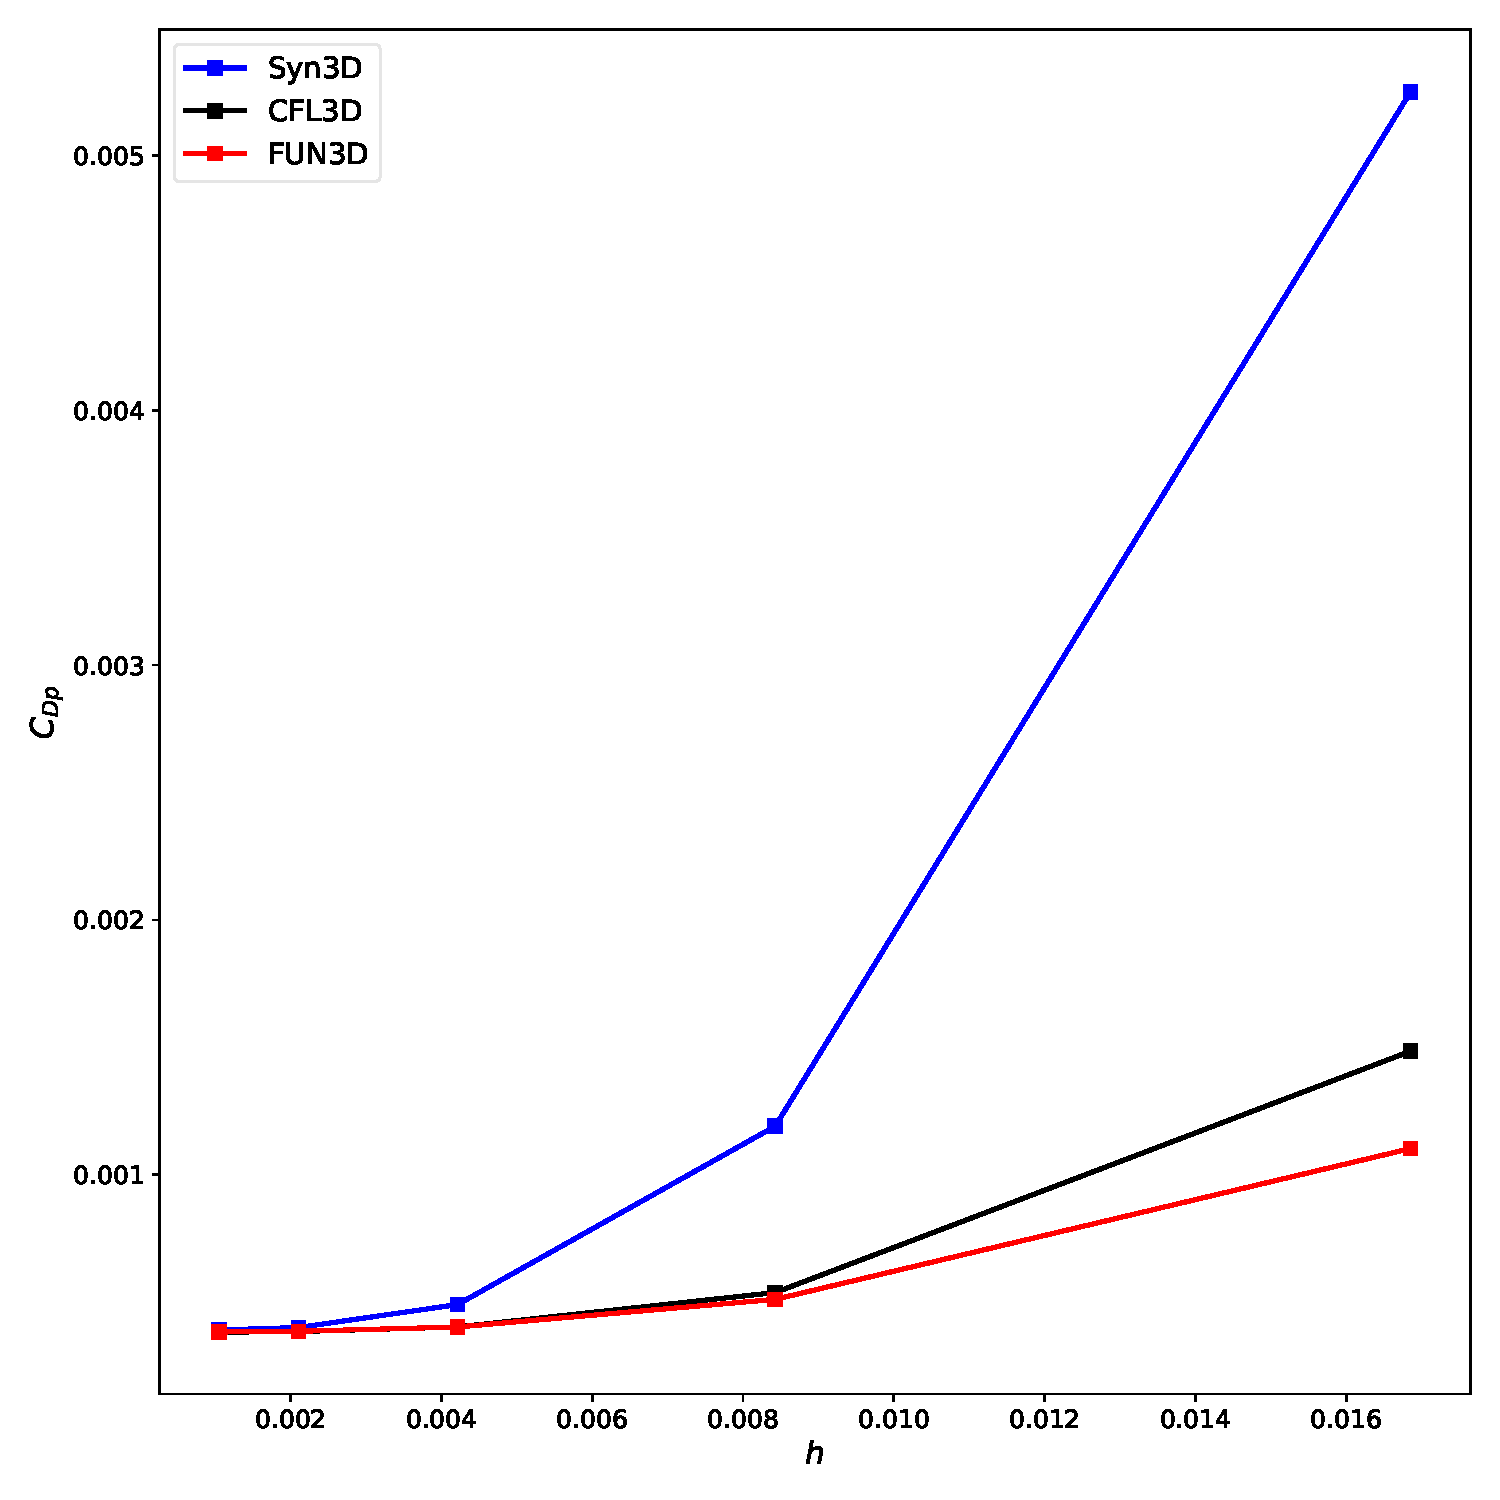
\includegraphics[width=1.0\textwidth]{figs/2dbump/C_DpGridStudy.pdf}
  \caption{Pressure contribution to drag.}
\end{subfigure}%
\begin{subfigure}{.45\textwidth}
  \centering
  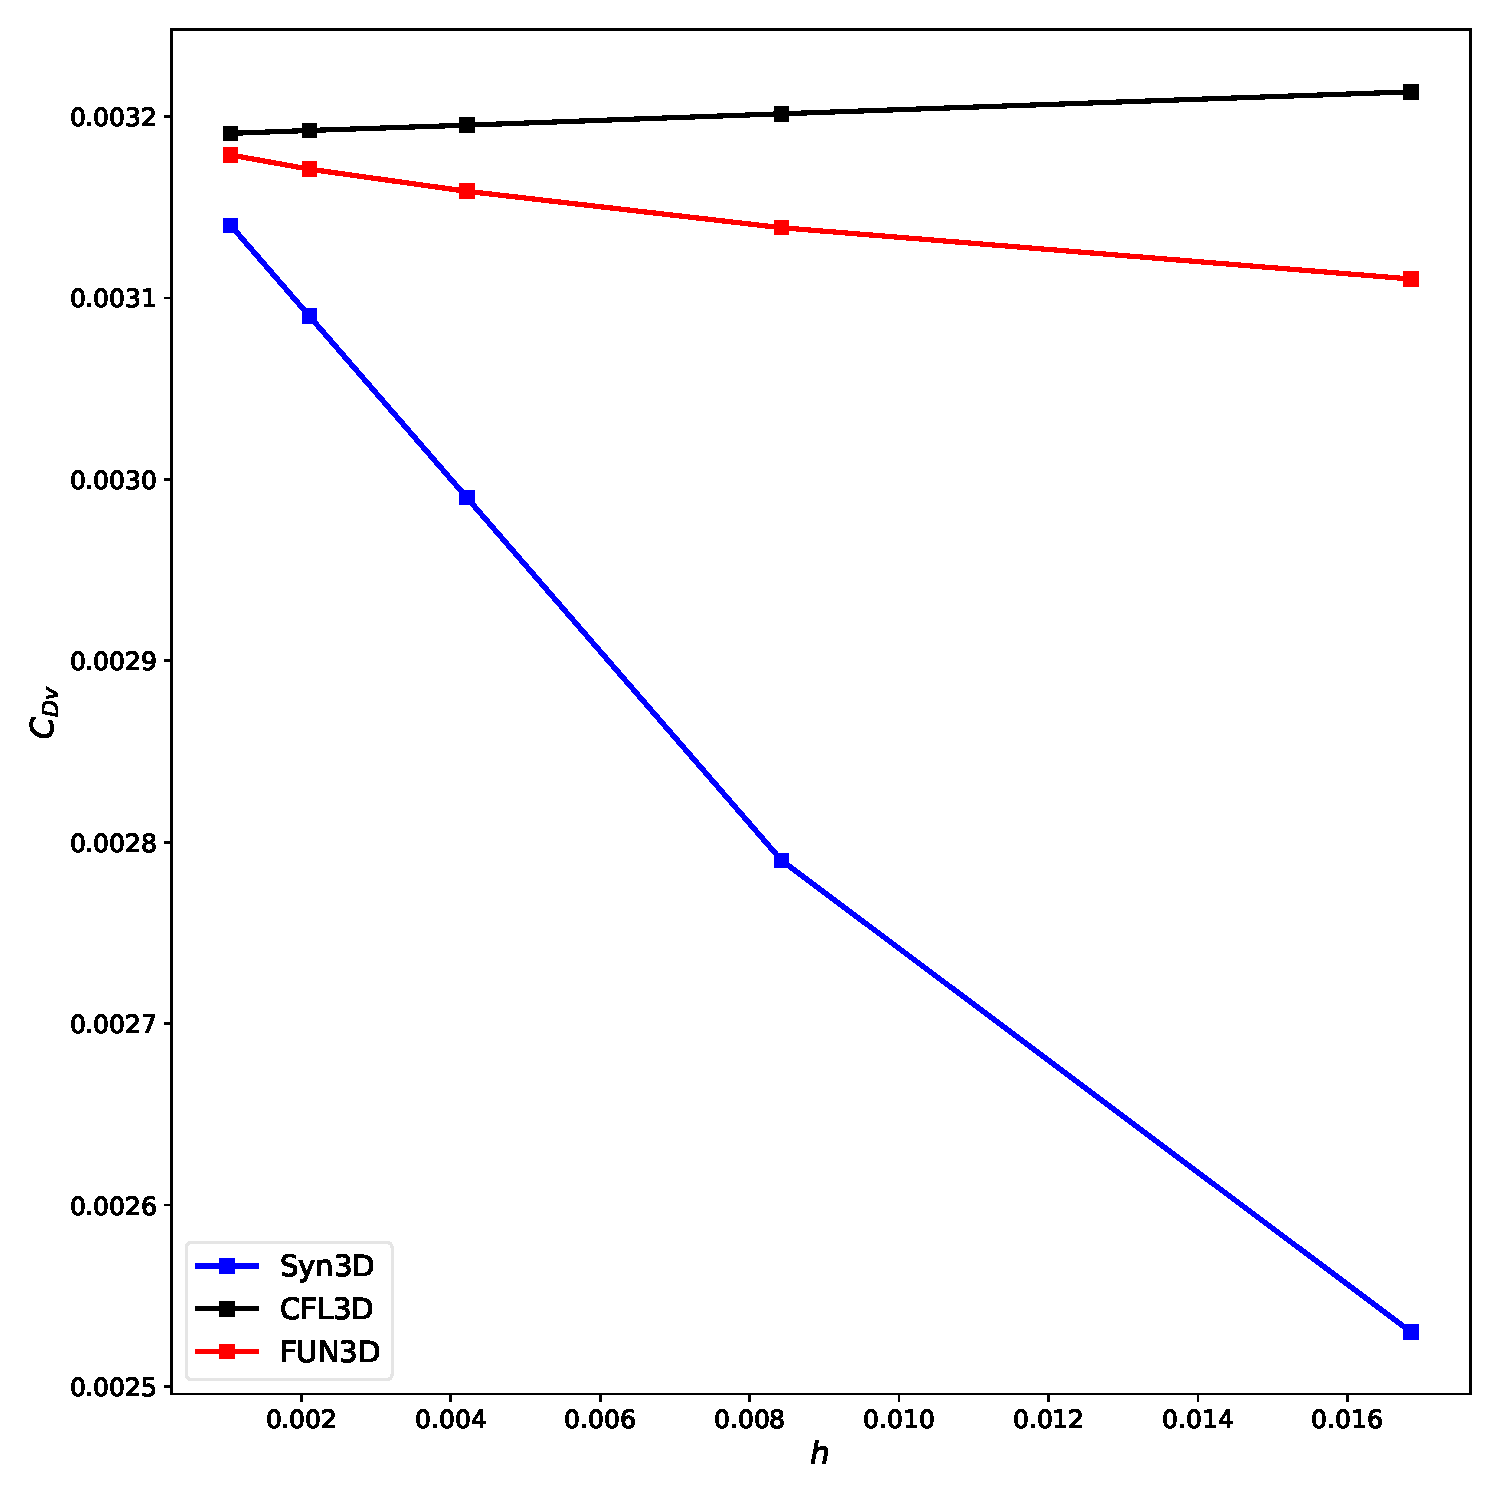
\includegraphics[width=1.0\textwidth]{figs/2dbump/C_DvGridStudy.pdf}
  \caption{Viscous contribution to drag.}
\end{subfigure}
\caption{2D Bump (syn3D): Force coefficients for various grid sizes.}
\label{fig:syn2dbumpforcestudy}
\end{figure}

\begin{figure}[ht!]
\centering
\begin{subfigure}{.45\textwidth}
  \centering
  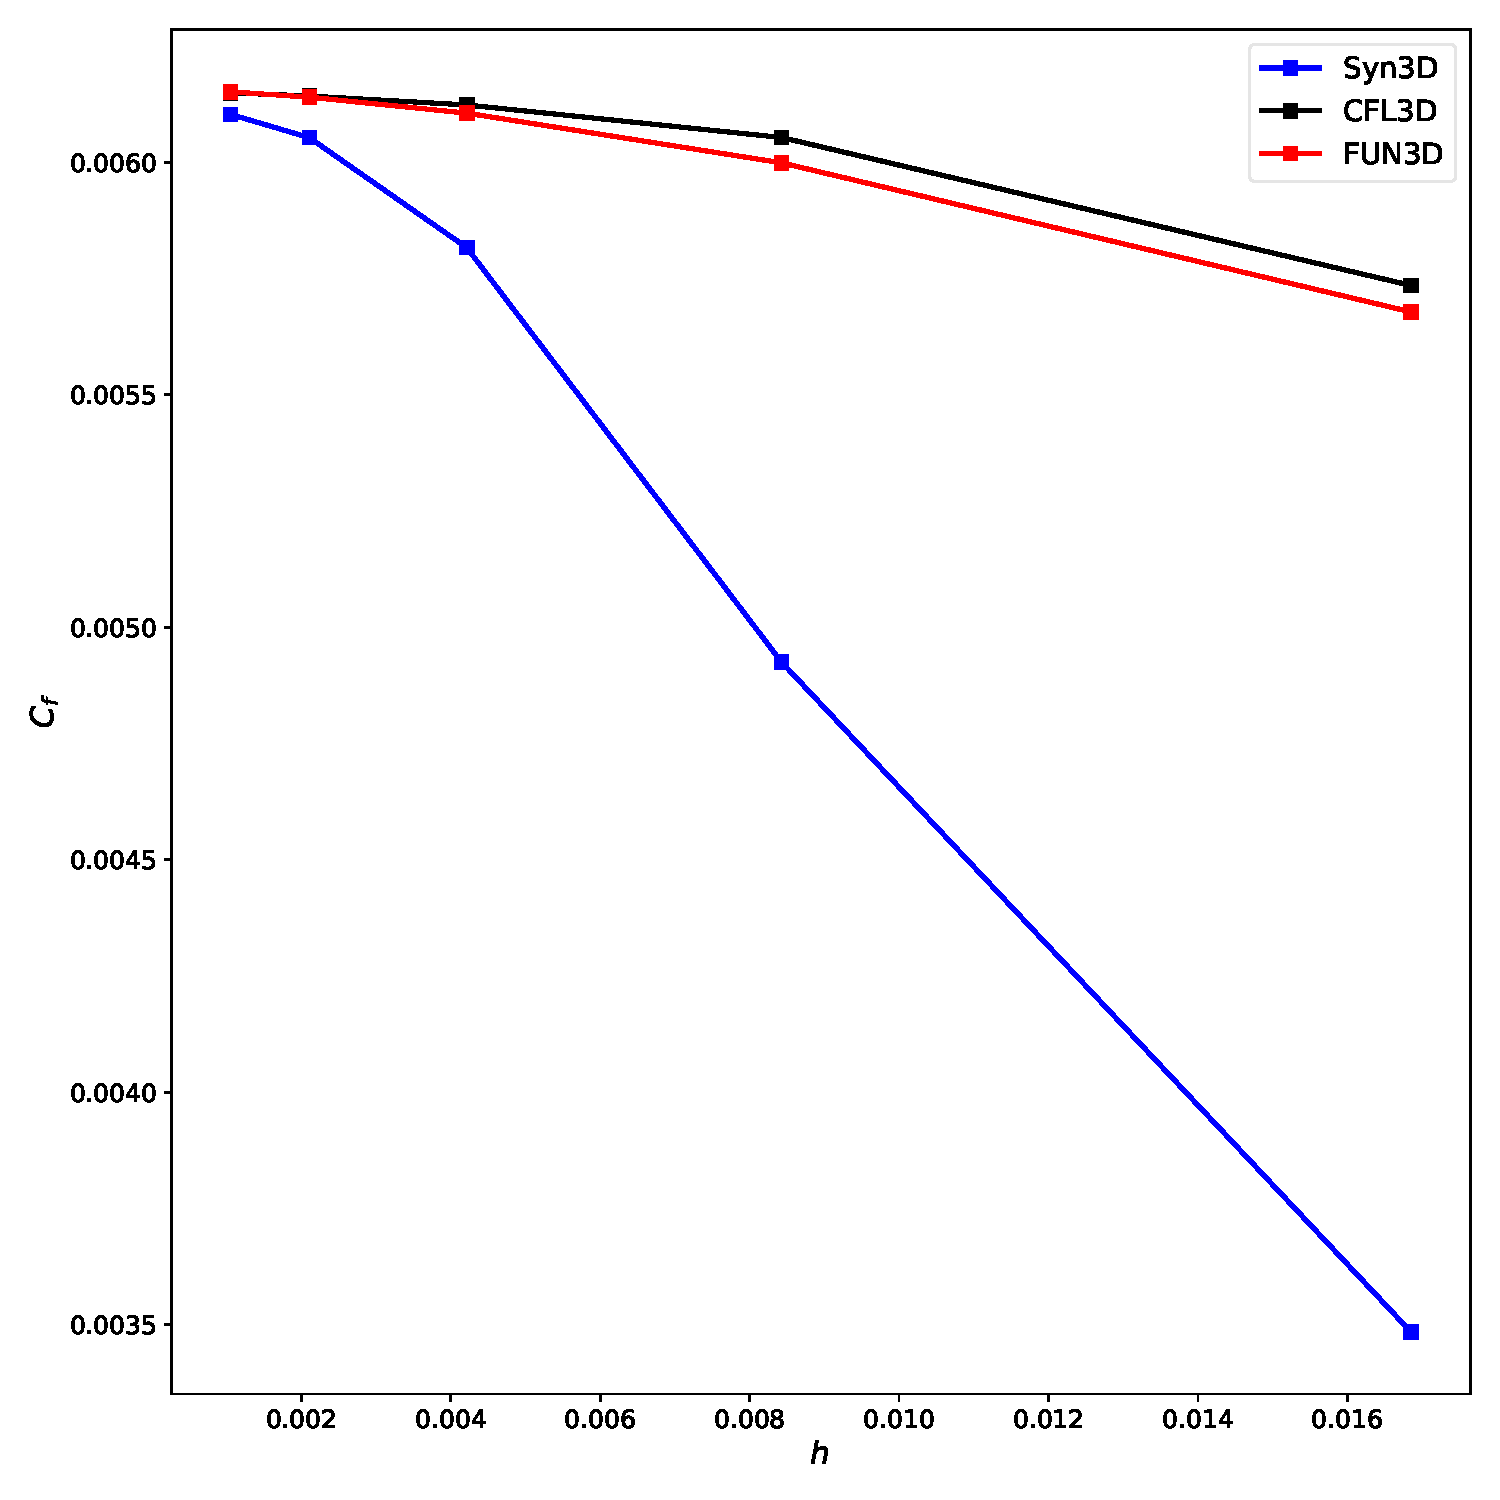
\includegraphics[width=1.0\textwidth]{figs/2dbump/Cf075GridStudy.pdf}
  \caption{$C_f$ grid study where x=0.75}
\end{subfigure}%
\begin{subfigure}{.45\textwidth}
  \centering
  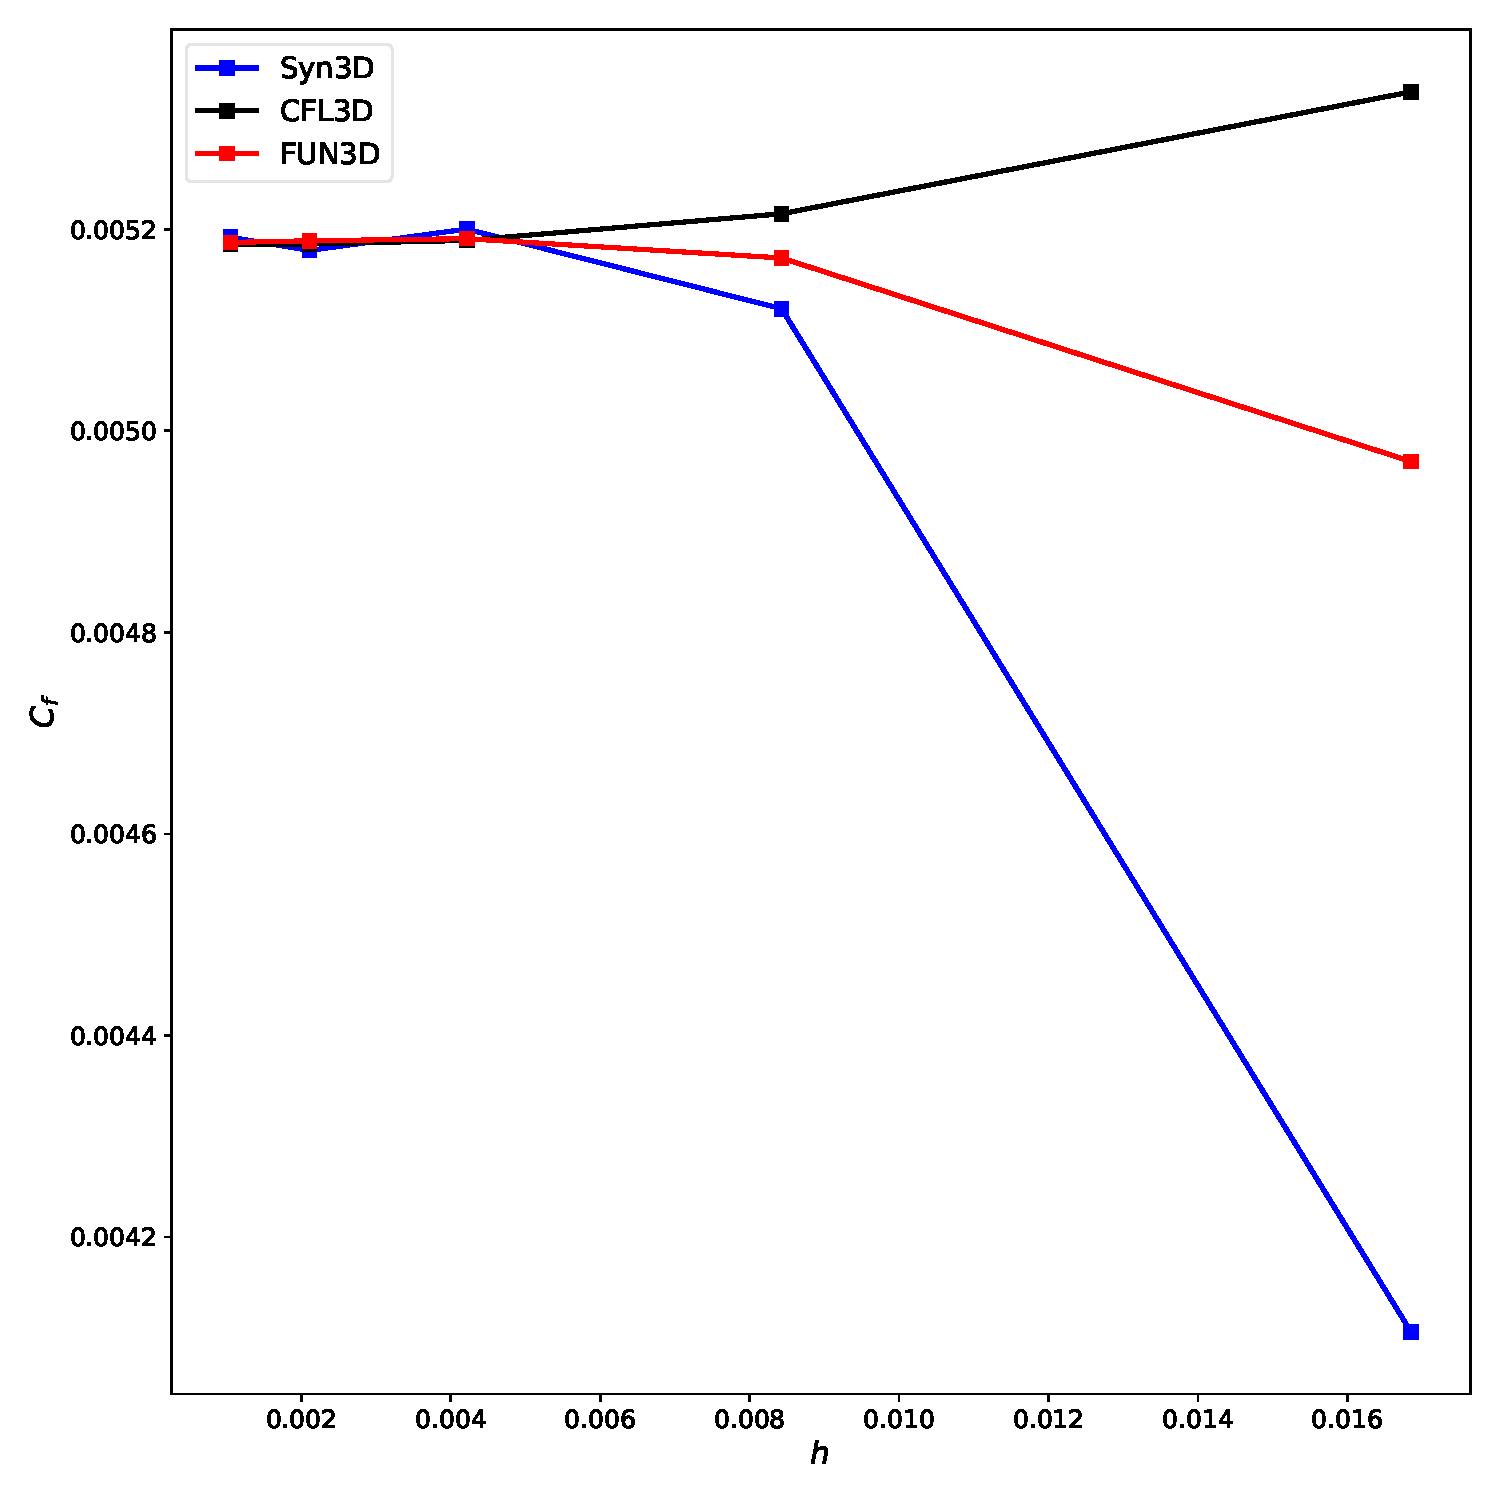
\includegraphics[width=1.0\textwidth]{figs/2dbump/Cf06321975GridStudy.pdf}
  \caption{$C_f$ grid study where x=0.6321975}
\end{subfigure}
\\
\begin{subfigure}{.45\textwidth}
  \centering
  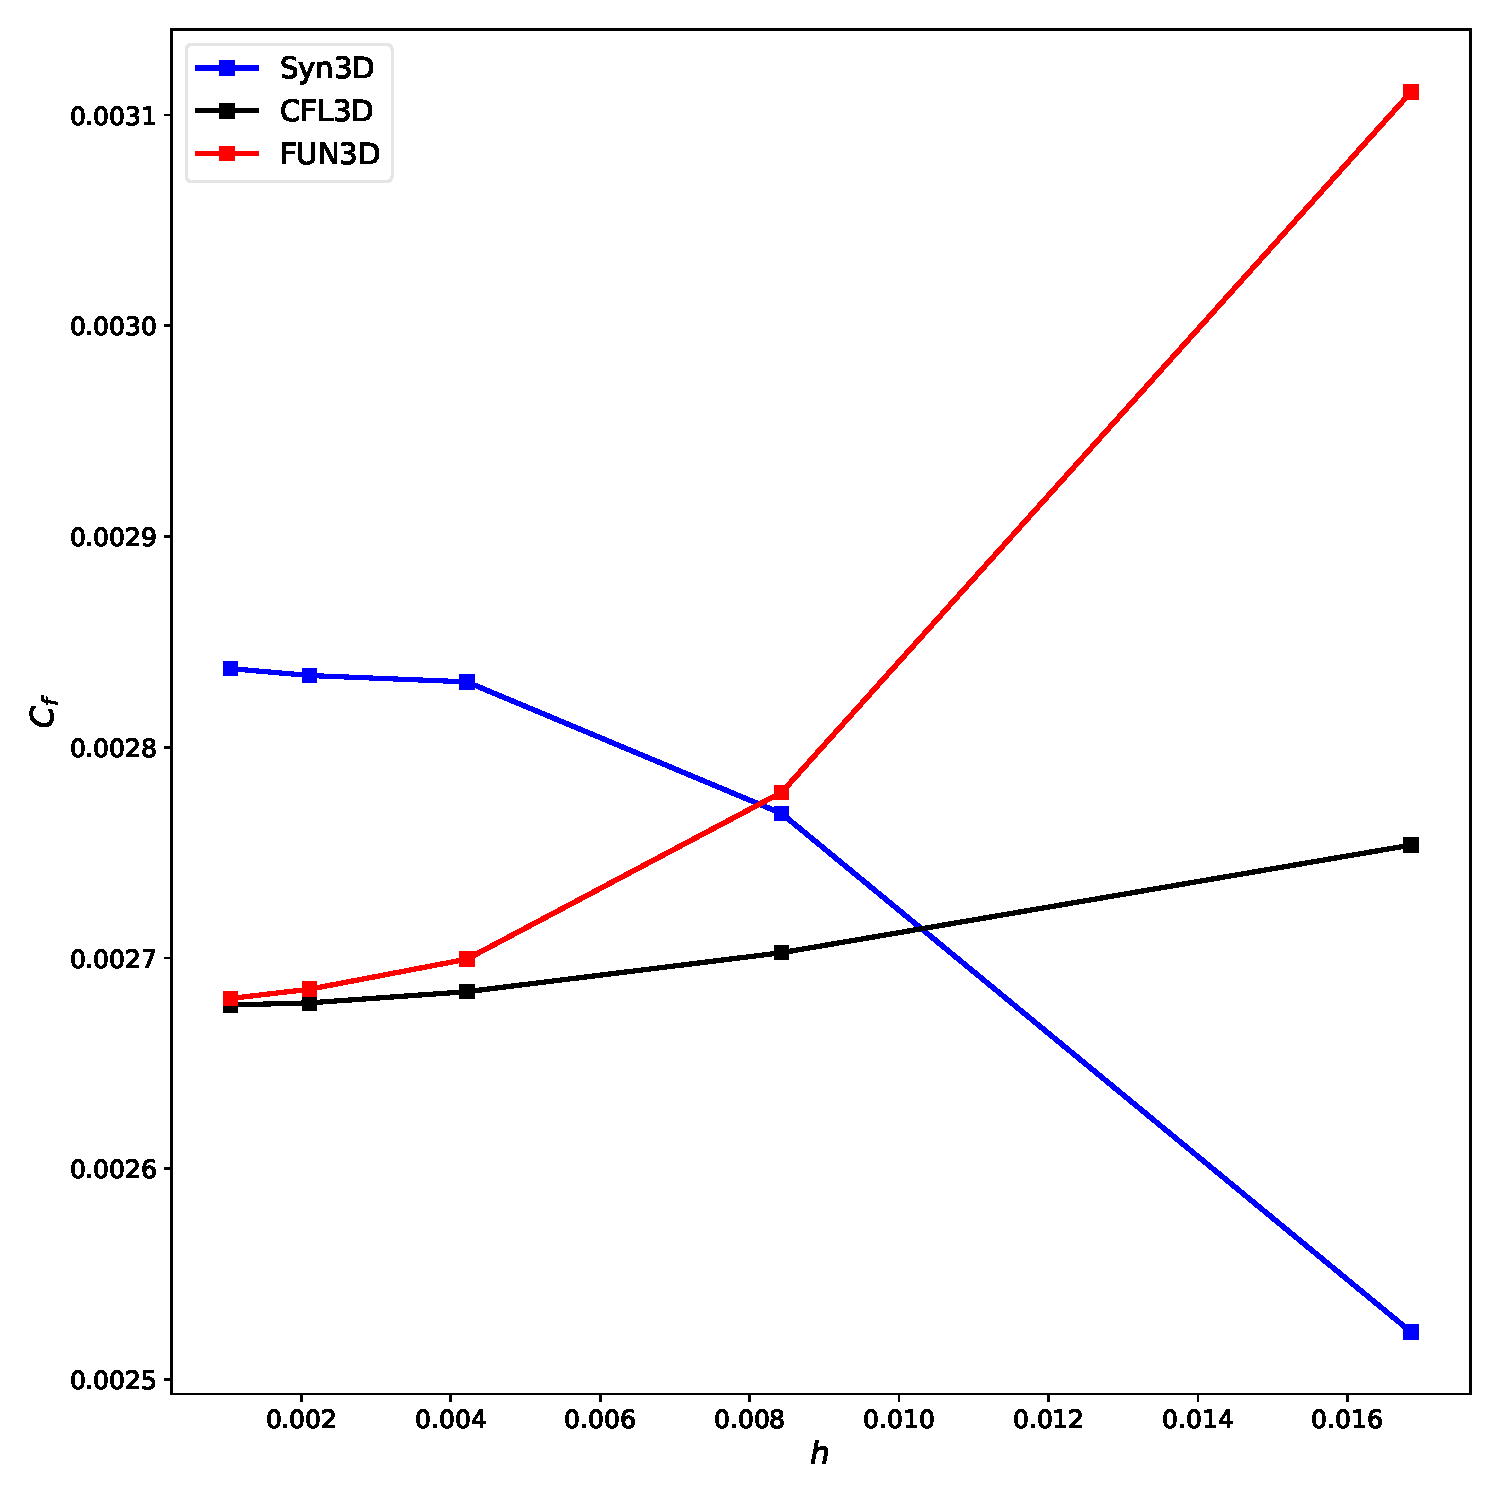
\includegraphics[width=1.0\textwidth]{figs/2dbump/Cf08678025GridStudy.pdf}
  \caption{$C_f$ grid study where x=0.8678025}
\end{subfigure}%}
\caption{2D Bump (syn3D): Skin friction coefficient at specific locations for various grid sizes.}
\label{fig:syn2dbumpcflocstudy}
\end{figure}

\Cref{fig:syn2dbumpcfstudy,fig:syn2dbumpcpstudy} show $C_f$ and $C_p$ distributions along the bump for all grids. Both plots show over-dissipated results for the coarser grids, which is expected, as discussed for the flat plate case. The difference of $C_f$ between the coarsest and finest grid is much greater than that of $C_p$. In other words, pressure seems to be less senstivive to mesh refinement than the skin friction. By the same token, while there is seemingly no difference of $C_p$ between the second finest and finest grids, indicating that grid convergence is achieved, there remains a noticeable discrepancy for $C_f$, which indicates its greater sensitivity to grid refinement.

\Cref{fig:syn2dbumpmutstudy} compares the eddy viscosity distribution between grids. The peak at the leading edge is significantly more pronounced for the coarser grids, and even slightly extends upstream. This results in over-predicted values for most, but not all, of the length of the wall; $\mu_t$ is under-predicted after $x\approx1.0$. Again, this is due to increased dissipation in the coarser grids, where the gradients are not as sharp as they should be.

\Cref{fig:syn2dbumpforcestudy,fig:syn2dbumpcflocstudy} show the convergence of force coefficients and skin friction for various grid sizes, compared with results from CFL3D and FUN3D. Again, it can be seen that there is much more dependence on grid size for syn3D as compared to the NASA solvers, although most values are very similar on the finest grid. The pressure contribution to drag, seems to have reached the asymptotic range of convergence, although the same cannot be said of the viscous contribution. Without a doubt, this increased dependence on grid size is due to the peak in eddy viscosity at the leading edge, which is an interface between block boundaries.

\section{Three-dimensional bump-in-channel}
\label{sec:syn3dbump}
The third verification case from the TMR website that was investigated was the three-dimensional bump-in-channel, which is available on~\cite{tmr} under the name ``3D Bump-in-channel''. This case was only simulated with syn3D.

The problem domain and flow conditions are shown in~\Cref{fig:3dbump}. While the website provides five sets of grids for this case as well, only results from the finest three grids are shown.
\begin{figure}
    \centering
    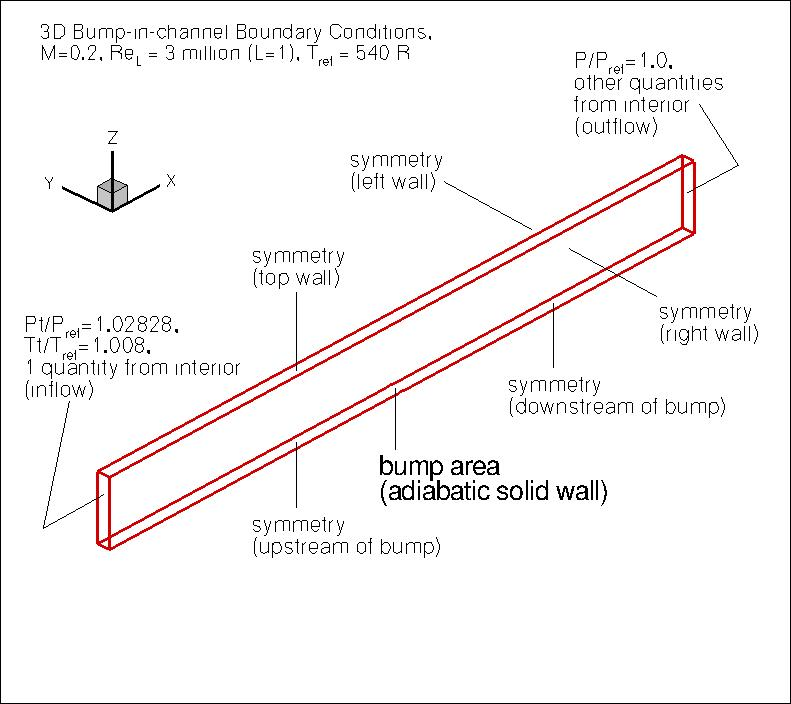
\includegraphics[width=0.7\textwidth]{figs/3dbump/bump3dBCpic1.jpg}
    \caption{Turbulent three-dimensional bump case~\cite{tmr}.}
    \label{fig:3dbump}
\end{figure}

The number of elements of the finest available grid exceeds 1.5 million and the residual could not be converged past $10^{-2}$ after over 6 days of computation with 64 cores, which is typically not sufficient for the purposes of verification -- results are shown nonetheless.

\Cref{tab:syn3dbump} compares force coefficients and shows relatively good agreement. \Cref{fig:syn3dbumpcnv} shows the convergence for the finest three grids.
\begin{table}[ht!]
\centering
\caption{3D Bump (syn3D): Comparison of force coefficients for the three-dimensional bump.}
\label{tab:syn3dbump}
\begin{tabular}{@{}l cccc@{}}
\toprule
Solver & $C_L$ & $C_D$ & $C_{Dv}$ & $C_{Dp}$ \\  \midrule
CFL3D & 0.0250 & 0.0036  & 0.0032 & 0.0004  \\
syn3D &  0.0258 & 0.0035  & 0.0031 & 0.0004  \\
\bottomrule
\end{tabular}
\end{table}
 \begin{figure}[ht!]
\centering
\begin{subfigure}{.45\textwidth}
  \centering
  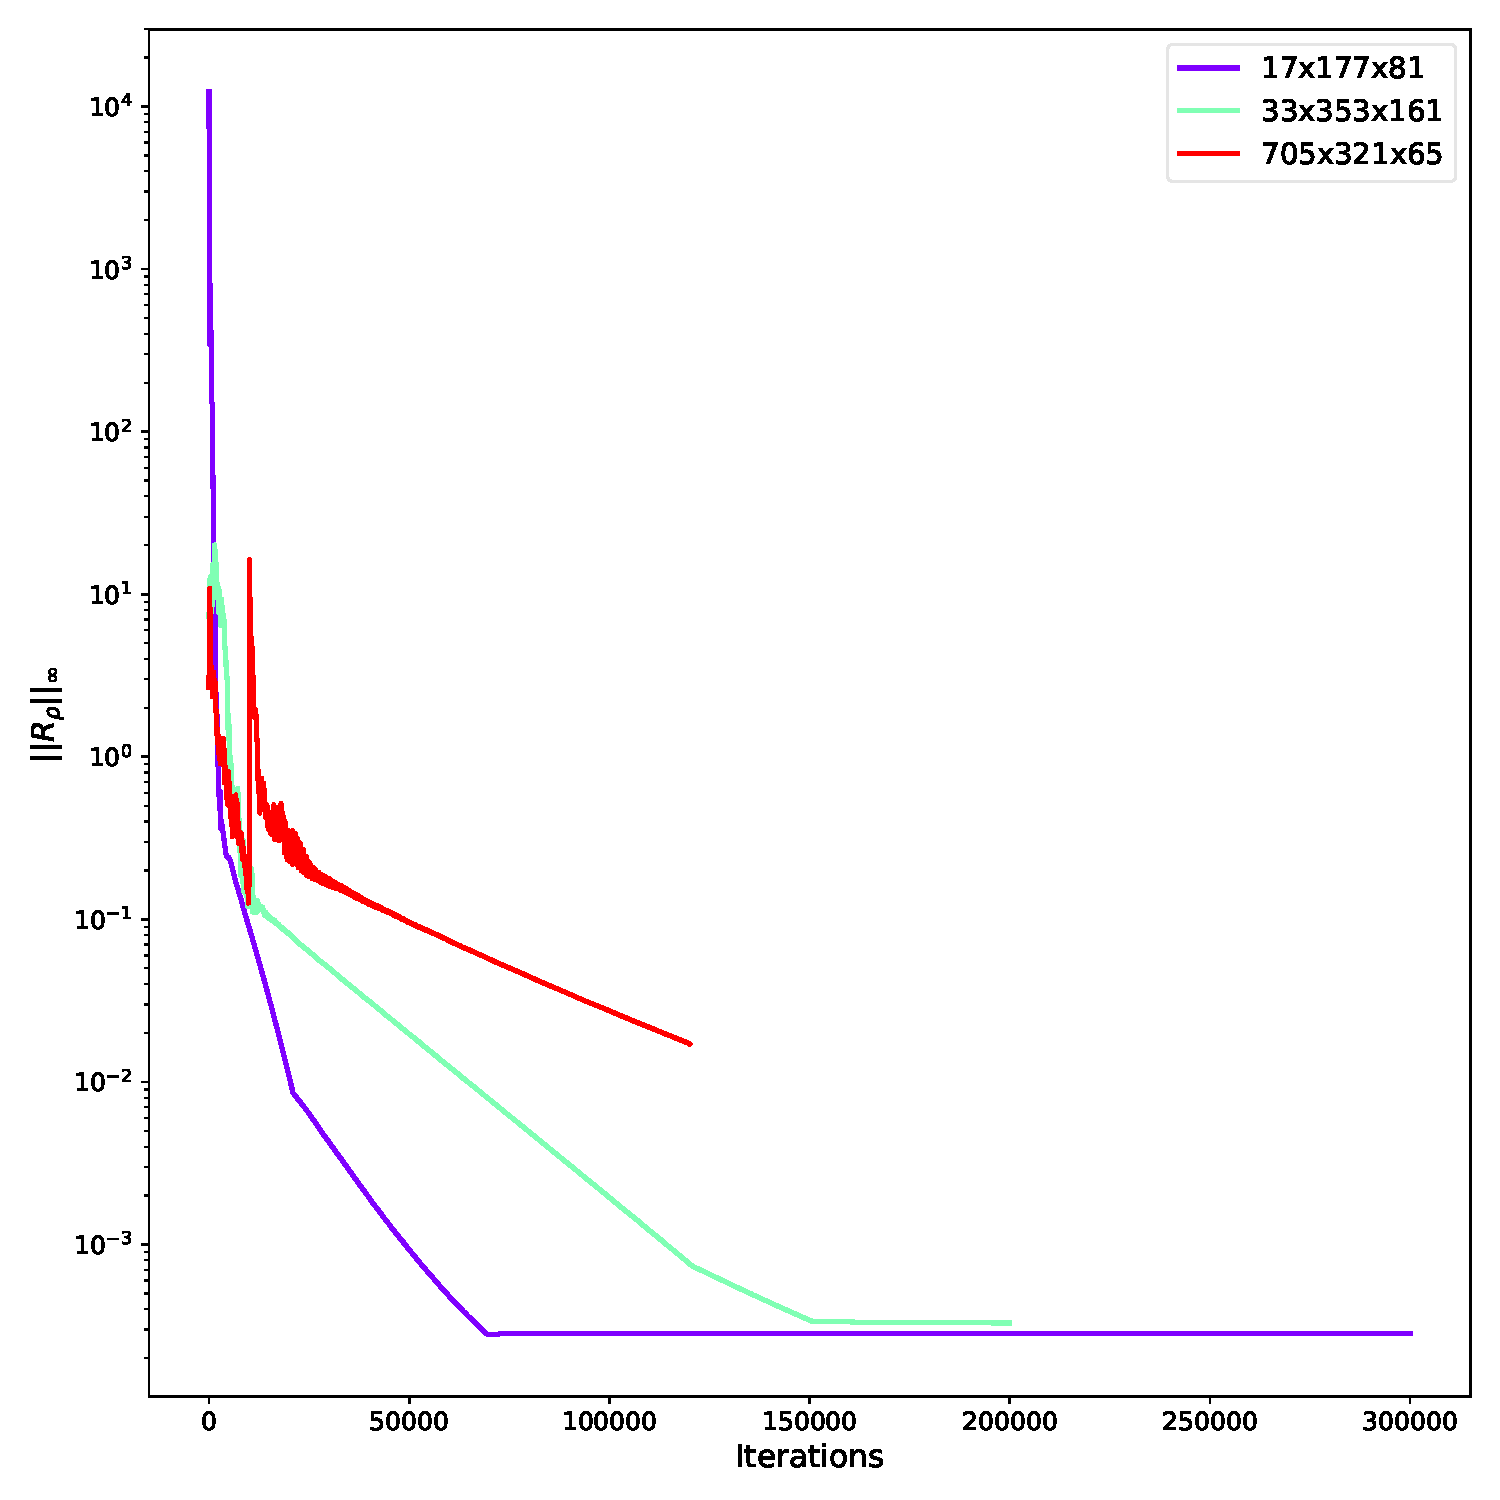
\includegraphics[width=1.0\textwidth]{figs/3dbump/convergenceRho.pdf}
  \caption{Maximum density residual.}
\end{subfigure}%
\begin{subfigure}{.45\textwidth}
  \centering
  \includegraphics[width=1.0\textwidth]{figs/3dbump/convergencesa.pdf}
  \caption{Maximum turbulent variable residual.}
\end{subfigure}
\caption{3D Bump (syn3D): Convergence of flow and turbulence variables.}
\label{fig:syn3dbumpcnv}
\end{figure}

 \begin{figure}[ht!]
\centering
\begin{subfigure}{.45\textwidth}
  \centering
  \includegraphics[width=1.0\textwidth]{figs/3dbump/cop001.pdf}
  \caption{$y=0.01$}
\end{subfigure}%
\begin{subfigure}{.45\textwidth}
  \centering
  \includegraphics[width=1.0\textwidth]{figs/3dbump/cop015.pdf}
  \caption{$y=0.15$}
\end{subfigure}
\\
\begin{subfigure}{.45\textwidth}
  \centering
  \includegraphics[width=1.0\textwidth]{figs/3dbump/cop030.pdf}
  \caption{$y=0.3$}
\end{subfigure}%
\begin{subfigure}{.45\textwidth}
  \centering
  \includegraphics[width=1.0\textwidth]{figs/3dbump/cop050.pdf}
  \caption{$y=0.50$}
\end{subfigure}
\caption{3D Bump (syn3D): Comparison of coefficient of pressure distribution at various cross-sections.}
\label{fig:syn3dbumpcp}
\end{figure}
\Cref{fig:syn3dbumpcp} compares $C_p$ at four fixed values of $y$. \Cref{fig:syn3dbumpmut03,fig:syn3dbumpmut12} show contour plots of the dimensionless eddy viscosity at $x=0.3$ and $x=1.2$ respectively. \Cref{fig:syn3dbumpmut} compares dimensionless eddy viscosity profiles at various locations. The plots are similar in trend to those of the two-dimensional bump, but vary due to the three-dimensional geometry of the bump. While the eddy viscosity is, as in previous cases, over-predicted by syn3D, \Cref{fig:syn3dbumpbad} displays a large discrepancy between syn3D and CFL3D.

\begin{figure}[ht!]
\centering
\begin{subfigure}{.45\textwidth}
  \centering
  \includegraphics[width=1.0\textwidth]{figs/3dbump/mut_03_cfl3d.jpg}
  \caption{CFL3D}
\end{subfigure}%
\begin{subfigure}{.45\textwidth}
  \centering
  \includegraphics[width=1.0\textwidth]{figs/3dbump/x03Rev.png}
  \caption{syn3D}
\end{subfigure}
\caption{3D Bump (syn3D): Contours of $\frac{\mu_t}{\mu_{\infty}}$ at $x=0.3$}
\label{fig:syn3dbumpmut03}
\end{figure}

\begin{figure}[ht!]
\centering
\begin{subfigure}{.45\textwidth}
  \centering
  \includegraphics[width=1.0\textwidth]{figs/3dbump/mut_12_cfl3d.jpg}
  \caption{CFL3D}
\end{subfigure}%
\begin{subfigure}{.45\textwidth}
  \centering
  \includegraphics[width=1.0\textwidth]{figs/3dbump/x12Rev.png}
  \caption{syn3D}
\end{subfigure}
\caption{3D Bump (syn3D): Contours of $\frac{\mu_t}{\mu_{\infty}}$ at $x=1.2$}
\label{fig:syn3dbumpmut12}
\end{figure}

\begin{figure}[ht!]
\centering
\begin{subfigure}{.45\textwidth}
  \centering
  \includegraphics[width=1.0\textwidth]{figs/3dbump/x03y01REV.pdf}
  \caption{$x=0.3, y=-0.1$}
\end{subfigure}%
\begin{subfigure}{.45\textwidth}
  \centering
  \includegraphics[width=1.0\textwidth]{figs/3dbump/x03y05REV.pdf}
  \caption{$x=0.3, y=-0.5$}
  \label{fig:syn3dbumpbad}
\end{subfigure}%
\\
\begin{subfigure}{.45\textwidth}
  \centering
  \includegraphics[width=1.0\textwidth]{figs/3dbump/x12y01REV.pdf}
  \caption{$x=1.2, y=-0.1$}
\end{subfigure}%
\begin{subfigure}{.45\textwidth}
  \centering
  \includegraphics[width=1.0\textwidth]{figs/3dbump/x12y05REV.pdf}
  \caption{$x=1.2, y=-0.5$}
\end{subfigure}%
\caption{3D Bump (syn3D): Comparison of dimensionless eddy viscosity profiles at various locations.}
\label{fig:syn3dbumpmut}
\end{figure}

As for the grid study, \Cref{fig:syn3dbumpforces} compares the dependence of force coefficients on grid size, \Cref{fig:syn3dbumpmutstudy} and \Cref{fig:syn3dbumpcpstudy} compare the eddy viscosity and pressure coefficient at select locations.
\begin{figure}[ht!]
\centering
\begin{subfigure}{.45\textwidth}
  \centering
  \includegraphics[width=1.0\textwidth]{figs/3dbump/C_L_GridStudy.pdf}
  \caption{$C_L$}
\end{subfigure}%
\begin{subfigure}{.45\textwidth}
  \centering
  \includegraphics[width=1.0\textwidth]{figs/3dbump/C_D_GridStudy.pdf}
  \caption{$C_D$}
\end{subfigure}
\\
\begin{subfigure}{.45\textwidth}
  \centering
  \includegraphics[width=1.0\textwidth]{figs/3dbump/C_Dp_GridStudy.pdf}
  \caption{$C_{Dp}$}
\end{subfigure}%
\begin{subfigure}{.45\textwidth}
  \centering
  \includegraphics[width=1.0\textwidth]{figs/3dbump/C_Dv_GridStudy.pdf}
  \caption{$C_{Dv}$}
\end{subfigure}
\caption{3D Bump (syn3D): Force coefficients for various grids}
\label{fig:syn3dbumpforces}
\end{figure}

\begin{figure}[ht!]
    \centering
    \includegraphics[width=0.4\textwidth]{figs/3dbump/x03y01REV_study.pdf}
    \caption{3D Bump (syn3D): Dimensionless eddy viscosity at $x=0.3,y=0.1$ for various grids.}
    \label{fig:syn3dbumpmutstudy}
\end{figure}

\begin{figure}[ht!]
    \centering
    \includegraphics[width=0.4\textwidth]{figs/3dbump/cop050study.pdf}
    \caption{3D Bump (syn3D): Coefficient of pressure at $y=0.5$ for various grids.}
    \label{fig:syn3dbumpcpstudy}
\end{figure}
\section{NACA0012}
The last validation case from the TMR website is the NACA 0012 airfoil case, which was only run with NX Flow. This case is available on~\cite{tmr} under the name ``2D NACA 0012 airfoil''. While the Turbulence Modeling Resource provides grids for this problem, they are not suitable for the boundary conditions available in NX Flow. The mesh used is shown in~\Cref{fig:naca0012}, which is an unstructured mesh. The boundary layer is meshed with hexahedron elements and the far field with tetrahedral elements. The average value of $y^+$ for the first layer is approximately unity. No grid study was performed since no grid study data is available at~\cite{tmr}.
\begin{figure}
    \centering
    \includegraphics[width=0.5\textwidth]{figs/naca0012/naca0012.png}
    \caption{Close-up of the NACA0012 unstructured mesh. Far field extends 3 chords upstream, 7 chords downstream and 3 chords above and below.}
    \label{fig:naca0012}
\end{figure}
This case was run using a fixed density, as it is an incompressible case. The Reynolds number value is 6 million and three angles of attack were used: 0, 10 and 15 degrees.

\Cref{tab:naca0012} tabulates the lift and drag coefficients at all angles of attack and \Cref{fig:naca0012_0} through \Cref{fig:naca0012_15} compare the pressure and skin friction coefficient along the airfoil at $\alpha=0\degc$, $\alpha=10\degc$ and $\alpha=15\degc$ respectively. In all cases, there is a high level of suction on the upper surface at the leading edge, as the flow accelerates. The pressure differential between the upper and lower surface is, for the most part, what generates lift. The skin friction distribution is, as expected, qualitatively similar to that of the flat plate.

Even though there is decent agreement between the coefficients of pressure and skin friction, the drag values are heavily over-predicted by NX Flow. The pressure at the leading edge is under-predicted by NX Flow. Compounded with the fact that most of the drag (over 90\%) is due to the pressure forces in this case, this results in the large discrepancy observed.
\begin{table}
    \centering
    \caption{NACA0012: Comparison of drag and lift coefficients at all angles of attack.}
    \label{tab:naca0012}
    \begin{tabular}{@{}l cc c cc c cc@{}}
        \toprule
         & \multicolumn{2}{c}{$\alpha = 0\degc$} & \phantom{a}
            & \multicolumn{2}{c}{$\alpha = 10\degc$} & \phantom{a}
            & \multicolumn{2}{c}{$\alpha = 15\degc$}\\
        \cline{2-3} \cline{5-6} \cline{8-9}
        Code & $C_L$ & $C_D$ && $C_L$ & $C_D$ && $C_L$ & $C_D$ \\
        \midrule
        CFL3D & $\approx$ 0 & 0.00819 && 1.0909 & 0.01231 && 1.5461 & 0.02124 \\
        FUN3D & $\approx$ 0 & 0.00812 && 1.0983 & 0.01242 && 1.5547 & 0.02159 \\
        NX Flow & 7.5E-5    & 0.01230 && 1.0175 & 0.05018 && 1.4295 & 0.09959 \\
        \bottomrule
    \end{tabular}
\end{table}

\begin{figure}[ht!]
\centering
\begin{subfigure}{.45\textwidth}
  \centering
  \includegraphics[width=1.0\textwidth]{figs/naca0012/cp_0.pdf}
  \caption{Coefficient of pressure.}
\end{subfigure}%
\begin{subfigure}{.45\textwidth}
  \centering
  \includegraphics[width=1.0\textwidth]{figs/naca0012/cf_0.pdf}
  \caption{Coefficient of skin friction.}
\end{subfigure}
\caption{NACA0012 (NX Flow): Force coefficient distribution at $\alpha = 0\degc$.}
\label{fig:naca0012_0}
\end{figure}

\begin{figure}[ht!]
\centering
\begin{subfigure}{.45\textwidth}
  \centering
  \includegraphics[width=1.0\textwidth]{figs/naca0012/cp_10.pdf}
  \caption{Coefficient of pressure.}
\end{subfigure}%
\begin{subfigure}{.45\textwidth}
  \centering
  \includegraphics[width=1.0\textwidth]{figs/naca0012/cf_10.pdf}
  \caption{Coefficient of skin friction.}
\end{subfigure}
\caption{NACA0012 (NX Flow): Force coefficient distribution at $\alpha = 10\degc$.}
\label{fig:naca0012_10}
\end{figure}

\begin{figure}[ht!]
\centering
\begin{subfigure}{.45\textwidth}
  \centering
  \includegraphics[width=1.0\textwidth]{figs/naca0012/cp_15.pdf}
  \caption{Coefficient of pressure.}
\end{subfigure}%
\begin{subfigure}{.45\textwidth}
  \centering
  \includegraphics[width=1.0\textwidth]{figs/naca0012/cf_15.pdf}
  \caption{Coefficient of skin friction.}
\end{subfigure}
\caption{NACA0012 (NX Flow): Force coefficient distribution at $\alpha = 15\degc$.}
\label{fig:naca0012_15}
\end{figure}

\section{RAE 2822}
Flow over the RAE 2822 airfoil is discussed in this section. Experimental data is obtained from the AGARD advisory report 138~\cite{agard}. The report provides results for a large set of conditions, however only two of these are run in this report: cases 3 and 9. The free-stream conditions and the solvers ran are tabulated in~\Cref{tab:raecases}. \Cref{fig:raesynmesh,fig:raenxmesh} show the mesh used in syn3D and NX Flow respectively. The average $y^+$ of the first layer for both grids is around 1.
\begin{table}
    \centering
    \caption{Case specifications for the RAE 2822 and which code they were run with.}
    \label{tab:raecases}
    \begin{tabular}{@{}l ccc cc@{}}
    \toprule
    Case & $M_\infty$ & $\Rey \times 10^{6}$ & $\alpha$ (\degc) & syn3D & NX Flow \\
    \midrule
    3 & 0.6 & 6.3 & 2.57 & Yes & Yes \\
    9 & 0.730 & 6.5 & 3.19 & Yes & No \\
    \bottomrule
    \end{tabular}
\end{table}
\begin{figure}
    \centering
    \includegraphics[width=0.7\textwidth]{figs/rae/synrae}
    \caption{Close-up of the syn3D mesh for the RAE 2822 case.}
    \label{fig:raesynmesh}
\end{figure}
\begin{figure}
    \centering
    \includegraphics[width=0.7\textwidth]{figs/rae/nxrae}
    \caption{Close-up of the NX Flow mesh for the RAE 2822 case.}
    \label{fig:raenxmesh}
\end{figure}
%
%
\subsection{Case 3}
%
%
\Cref{fig:raecp3} compares the pressure coefficient over the airfoil between NX Flow, syn3D and the experimental data. \Cref{fig:raecf3} compares the skin friction coefficient only for syn3D and NX Flow, since no experimental data is available. It can be seen that syn3D over-predicts the suction on the upper surface at the leading edge, whereas NX Flow under-predicts it. The skin friction coefficient distribution is different between syn3D and NX Flow, but similar trends can be observed.

\Cref{tab:raecase3} tabulates the lift and drag coefficients. Syn3D slightly over-predicts both the lift and drag, whereas NX Flow under-predicts the lift and significantly over-predicts drag, as it did for the NACA0012 case.
\begin{table}
    \centering
    \caption{RAE 2822 case 3 (syn3D \& NX Flow): Comparison of drag and lift coefficients with experimental data.}
    \label{tab:raecase3}
    \begin{tabular}{@{}lcc@{}}
        \toprule
        Source & $C_L$ & $C_D$ \\
        \midrule
        Experimental & 0.5220 & 0.0101 \\
        syn3D & 0.5907 & 0.0115 \\
        NX Flow & 0.4865 & 0.0348 \\
         \bottomrule
    \end{tabular}
\end{table}
\begin{figure}
    \centering
    \includegraphics[width=0.7\textwidth]{figs/rae/cp_case3}
    \caption{RAE 2822 case 3 (syn3D \& NX Flow): Coefficient of pressure along the airfoil.}
    \label{fig:raecp3}
\end{figure}
\begin{figure}
    \centering
    \includegraphics[width=0.7\textwidth]{figs/rae/cf_case3}
    \caption{RAE 2822 case 3 (syn3D \& NX Flow) : Coefficient of skin friction along the airfoil.}
    \label{fig:raecf3}
\end{figure}

\subsection{Case 9}
\Cref{fig:raecp9} compares the pressure coefficient over the airfoil between syn3D and experimental data. A shock can be observed on the upper surface, at around half of the chord length. This shock is well captured by syn3D and the location approximately matches that of the experimental data. \Cref{fig:raecf9} shows the skin friction coefficient on the upper surface. A shock can be observed in this plot as well, at around half the chord length.

\Cref{tab:raecase9} tabulates the lift and drag coefficients. Once again, syn3D slightly over-predicts both the lift and drag.
\begin{table}
    \centering
    \caption{RAE 2822 case 9 (syn3D): Comparison of drag and lift coefficients with experimental data.}
    \label{tab:raecase9}
    \begin{tabular}{@{}lcc@{}}
        \toprule
        Source & $C_L$ & $C_D$ \\
        \midrule
        Experimental & 0.8030 & 0.0168 \\
        syn3D & 0.8186 & 0.0225 \\
         \bottomrule
    \end{tabular}
\end{table}
\begin{figure}
    \centering
    \includegraphics[width=0.7\textwidth]{figs/rae/cp_case9}
    \caption{RAE 2822 case 9 (syn3D) : Coefficient of pressure along the airfoil.}
    \label{fig:raecp9}
\end{figure}
\begin{figure}
    \centering
    \includegraphics[width=0.7\textwidth]{figs/rae/cf_case9}
    \caption{RAE 2822 case 9 (syn3D) : Coefficient of skin friction along the upper surface of the airfoil.}
    \label{fig:raecf9}
\end{figure}

\section{High-lift configuration}
The last case that was run is the McDonnel-Douglas 30P/30N three-element high-lift configuration. This case was only run with syn3D and the mesh is shown in~\Cref{fig:highmesh}. \Cref{tab:high} tabulates the free-stream conditions.
\begin{table}
    \centering
    \caption{Specification of free-stream flow conditions for the high-lift configuration}
    \label{tab:high}
    \begin{tabular}{ccc}
        \toprule
        $M_\infty$ & $\Rey \times 10^6$ & $\alpha$ (\degc)\\
        \midrule
        0.2 & 9 & 19 \\
        \bottomrule
    \end{tabular}
\end{table}
\begin{figure}
    \centering
    \includegraphics[width=0.7\textwidth]{figs/high/highlift}
    \caption{High-lift (syn3D): Close-up of the high-lift mesh.}
    \label{fig:highmesh}
\end{figure}
Unfortunately, this case could only be run on a mesh with an average $y^+$ of 50 and composed of around 100,000 elements. Of course, this is much too coarse of a mesh, especially for such a complex configuration, but the results are qualitatively accurate nonetheless.

\Cref{fig:highdist} shows a contour of the wall distance. \Cref{fig:highstream} depicts streamlines around the airfoils, which shows the expected recirculation regions.

\Cref{fig:highcp} compares the coefficient of pressure distribution with ISAAC~\cite{morrison1998numerical}. The cited reference also shows experimental data, although the results from ISAAC are virtually identical. It can be seen that the suction on the first element is not as pronounced as it should be for syn3D, which can be attributed to the coarseness of the grid. ISAAC also implements a transitional model, which allows the flow to naturally transition between the laminar regime and turbulent regime. Such a model is currently not implemented in syn3D, and this is another source of error~\cite{morrison1998numerical}.

Finally, \Cref{tab:highld} compares the lift and drag coefficients. The lift coefficient is under-predicted and the drag coefficient is over-predicted. This discrepancy may be attributed to the reasons mentioned above.
\begin{figure}
    \centering
    \includegraphics[width=0.7\textwidth]{figs/high/high_dist}
    \caption{High-lift (syn3D): Wall distance contour.}
    \label{fig:highdist}
\end{figure}
\begin{figure}
    \centering
    \includegraphics[width=0.7\textwidth]{figs/high/highstream}
    \caption{High-lift (syn3D): Streamlines around the high-lift configuration. Recirculation regions are identified by the solid black shapes.}
    \label{fig:highstream}
\end{figure}
\begin{figure}
    \centering
    \includegraphics[width=0.95\textwidth]{figs/high/cp_highlift}
    \caption{High-lift (syn3D): Comparison of coefficient of pressure distribution.}
    \label{fig:highcp}
\end{figure}
\begin{table}
    \centering
    \caption{High-lift (syn3D): Comparison of lift and drag coefficients}
    \label{tab:highld}
    \begin{tabular}{l cc}
        \toprule
        Code & $C_L$ & $_D$ \\
        \midrule
        syn3D & 2.98 & 0.290\\
        ISAAC & $\approx$ 4 & $\approx$ 0.08\\
        \bottomrule
    \end{tabular}
\end{table}

%\section{Syn3D}
\label{sec:resultssyn}
Verification of the implementation of the Spalart-Allmaras turbulence model in Syn3D is verified in this section. First, the program is compared against established CFD codes on three different cases available on the Turbulence Modeling Resource (TMR) website~\cite{tmr}. Then, it is compared against experimental data on an RAE2822 airfoil. Finally, results for a multi-element airfoil configuration are shown.

\subsection{Flat plate}
The turbulent flow over a flat plate is investigated. All grids and results are available in~\cite{tmr} under the name: ``2D Zero pressure gradient flat plate''. The problem domain and flow conditions are shown in~\Cref{fig:flat}. The Turbulence Modeling Resource provides five grids, each finer than the next, in order to compare so-called mesh independent results and to perform a grid study. The goal of a grid study is to establish that the obtained results will not vary significantly by further refining the mesh. 
\begin{figure}
    \centering
    \includegraphics[width=0.7\textwidth]{figs/flat/flatplate.png}
    \caption{Turbulent flat plate case~\cite{tmr}.}
    \label{fig:flat}
\end{figure}
The skin friction coefficient $C_f$ at $x = 0.97$ and drag coefficient $C_D$ are compared to CFL3D, a cell-centered finite volume code developed by NASA, in~\Cref{tab:flat}. They are calculated as:
\begin{align*}
    C_f = \frac{2\tau_w}{\rho_\infty U_\infty^2}\\
    C_D = \frac{2D}{\rho_\infty U_\infty^2 A}
\end{align*}
where $D$ is the drag force and $A$ is the reference area. For this case, the reference area is the length of the plate times its width, i.e. the length of the mesh in the $z$ direction. \Cref{tab:flat} tabulates skin friction coefficient and drag coefficient values.
\begin{table}
\centering
\caption{Flat Plate (Syn3D): Comparison of force coefficients on the finest grid.}
\label{tab:flat}
\begin{tabular}{@{}lcc@{}}
    \toprule
    Solver & $C_D$ & $C_f$ at $x=0.97$ \\
    \midrule
    CFL3D & 0.00286 & 0.00270 \\
    Syn3D & 0.00280 & 0.00269\\
    \bottomrule
\end{tabular}
\end{table}
\Cref{fig:synflatcnvstudy} shows the residual convergence of the density residual and turbulence residual for all grids. The density residual, which is the residual of the mass equation, was driven down to around $10^-4$ on all meshes, which is enough for the sake of this comparison -- differences in the obtained solution field were found to be marginal beyond that point.
\begin{figure}[ht!]
\centering
\begin{subfigure}{.45\textwidth}
  \centering
  \includegraphics[width=1.0\textwidth]{figs/flat/gov_convergence_gridstudy.pdf}
  \caption{Maximum density residual.}
\end{subfigure}%
\begin{subfigure}{.45\textwidth}
    \centering
    \includegraphics[width=1.0\textwidth]{figs/flat/SA_convergence_gridstudy.pdf}
    \caption{Maximum turbulence variable residual.}
\end{subfigure}
\caption{Flat Plate (Syn3D): Convergence of flow and turbulence variables on various grid sizes.}
\label{fig:synflatcnvstudy}
\end{figure}
% \begin{figure}[ht!]
% \centering
% \begin{subfigure}{.45\textwidth}
%   \centering
%   \includegraphics[width=1.0\textwidth]{figs/flat/gov_convergence.pdf}
%   \caption{Maximum density residual}
% \end{subfigure}%
% \begin{subfigure}{.45\textwidth}
%   \centering
%   \includegraphics[width=1.0\textwidth]{figs/flat/turb_convergence.pdf}
%   \caption{Maximum turbulent variable residuals}
% \end{subfigure}
% \caption{Convergence of flow and turbulence variables (finest flat plate).}
% \label{fig:synflatcnv}
% \end{figure}

Several plots have been generated to compare the results between Syn3D and CFL3D. Unless otherwise noted, all results were obtained with the finest grid. \Cref{fig:synflatcf} compares the skin friction along the plate. \Cref{fig:synflatmutcontour} shows contour plots of the dimensionless eddy viscosity $\frac{\mu_t}{\mu_{\infty}}$ and \Cref{fig:synflatmu} shows line plots of the dimensionless eddy viscosity. \Cref{fig:synflatu,fig:synflatupyp} show profiles of the dimensionless velocity $u/u_\infty$ and $u^+$ respectively. There is decent agreement between the two solvers, and the source of discrepancy is easily seen in~\Cref{fig:synflatmutmax}: the eddy viscosity jumps abruptly right at the leading edge for Syn3D but not for CFL3D. The cause of this jump was investigated by the author as well as others working on the code, but a definite answer was unfortunately not found.
\begin{figure}[ht!]
\centering
	\includegraphics[width=0.7\textwidth]{figs/flat/skin_friction.pdf}
    \caption{Flat Plate (Syn3D): Coefficient of skin friction along the plate.}
    \label{fig:synflatcf}
\end{figure}

\begin{figure}[ht!]
\centering
\begin{subfigure}{.45\textwidth}
  \centering
  \includegraphics[width=1.0\textwidth]{figs/flat/mut_contours_cfl3d.jpg}
  \caption{CFL3D}
\end{subfigure}%
\begin{subfigure}{.45\textwidth}
  \centering
  \includegraphics[width=1.0\textwidth]{figs/flat/rev_sa.png}
  \caption{Syn3D}
\end{subfigure}
\caption{Flat Plate (Syn3D): Contours of non-dimensionalized eddy viscosity}
\label{fig:synflatmutcontour}
\end{figure}

\begin{figure}[ht!]
\centering
\begin{subfigure}{.45\textwidth}
  \centering
  \includegraphics[width=1.0\textwidth]{figs/flat/mut_x097.pdf}
  \caption{Nondimensional eddy viscosity at x=0.97 }
\end{subfigure}%
\begin{subfigure}{.45\textwidth}
  \centering
  \includegraphics[width=1.0\textwidth]{figs/flat/maxmut.pdf}
  \caption{Maximum $\frac{\mu_t}{\mu_{\infty}}$ in the boundary layer}
  \label{fig:synflatmutmax}
\end{subfigure}
\caption{Flat Plate (Syn3D): Dimensionless eddy viscosity line plots}
\label{fig:synflatmu}
\end{figure}

\begin{figure}[ht!]
\centering
\begin{subfigure}{.45\textwidth}
  \centering
  \includegraphics[width=1.0\textwidth]{figs/flat/u097.pdf}
  \caption{$x=0.97$}
\end{subfigure}%
\begin{subfigure}{.45\textwidth}
  \centering
  \includegraphics[width=1.0\textwidth]{figs/flat/u190.pdf}
  \caption{$x=1.90$}
\end{subfigure}
\caption{Flat Plate (Syn3D): $\frac{U}{U_{\infty}}$ profiles in the boundary layer}
\label{fig:synflatu}
\end{figure}

\begin{figure}[ht!]
\centering
\begin{subfigure}{.45\textwidth}
  \centering
  \includegraphics[width=1.0\textwidth]{figs/flat/uplus_yplus_097.pdf}
  \caption{$x=0.97$}
\end{subfigure}%
\begin{subfigure}{.45\textwidth}
  \centering
  \includegraphics[width=1.0\textwidth]{figs/flat/uplus_yplus_190.pdf}
  \caption{$x=1.90$}
\end{subfigure}
\caption{Flat Plate (Syn3D): $u^+$ vs. $y^+$ profiles in the boundary layer. Law of the wall is also shown for comparison.}
\label{fig:synflatupyp}
\end{figure}

Next, \Cref{fig:synflatforcestudy} shows the dependence of $C_D$ and $C_f$ on the grid spacing $h = 1/N^2$, where $N$ is the number of grid points. It can be seen that there is still significant differences in results between the second finest and finest grid for Syn3D as compared to CFL3D and FUN3D -- the latter is a vertex-centered code also developed by NASA. \Cref{fig:synflatcnvstudy} shows the Syn3D convergence of residuals for all five grids. As expected, the coarser grids show faster convergence than the finer ones -- this phenomenon is detailed in~\cite{blazek2015computational}. \Cref{fig:synflatcfstudy,fig:synflatprofilestudy} show the variation of skin friction coefficient along the plate and profiles of eddy viscosity and velocity with grid size respectively. These plots show that the solution field seems to converge to a unique solution, as opposed to oscillating back and forth between different values.
\begin{figure}[ht!]
\centering
\begin{subfigure}{.45\textwidth}
  \centering
  \includegraphics[width=1.0\textwidth]{figs/flat/cd_grid.pdf}
  \caption{Coefficient of drag.}
\end{subfigure}%
\begin{subfigure}{.45\textwidth}
  \centering
  \includegraphics[width=1.0\textwidth]{figs/flat/cf_grid.pdf}
  \caption{Coefficient of Skin Friction at x=0.97.}
\end{subfigure}
\caption{Flat Plate (Syn3D): Force coefficients for various grid sizes.}
\label{fig:synflatforcestudy}
\end{figure}

\begin{figure}[ht!]
\centering
  \includegraphics[width=0.7\textwidth]{figs/flat/skin_friction_grid.pdf}
  \caption{Flat Plate (Syn3D): Coefficient of skin friction on various grids.}
  \label{fig:synflatcfstudy}
\end{figure}

\begin{figure}[ht!]
\centering
\begin{subfigure}{.45\textwidth}
  \centering
  \includegraphics[width=1.0\textwidth]{figs/flat/rev_grid.pdf}
  \caption{Dimensionless eddy viscosity}
\end{subfigure}%
\begin{subfigure}{.45\textwidth}
  \centering
  \includegraphics[width=1.0\textwidth]{figs/flat/u097_grid.pdf}
  \caption{Dimensionless velocity}
\end{subfigure}
\caption{Flat Plate (Syn3D): Profiles at $x=0.97$ for various grid sizes.}
\label{fig:synflatprofilestudy}
\end{figure}

\section{Two-dimensional bump-in-channel}
Upon completion of the validation of the flow over a flat-plate, the turbulent flow on a two-dimensional bump-in-channel case was investigated. This case is also available on~\cite{tmr} under the name ``2D Bump-in-channel''. This case was only run with syn3D.

The problem domain and flow conditions are shown in~\Cref{fig:2dbump}. It is referred to as two-dimensional due to the shape of the bump not depending upon the $z$ coordinate, as opposed to the three-dimensional bump in~\Cref{sec:syn3dbump}.

This case is different from the previous flat plate case because it involves wall curvature, which induces a pressure gradient. The TMR website also provides five grids for this case.
\begin{figure}
    \centering
    \includegraphics[width=0.7\textwidth]{figs/2dbump/bumpBCpic.jpg}
    \caption{Turbulent two-dimensional bump case~\cite{tmr}.}
    \label{fig:2dbump}
\end{figure}

\begin{table}[ht!]
    \centering
    \caption{2D Bump (syn3D): Comparison of force coefficients for the finest two-dimensional bump.}
\label{tab:syn2dbump1}
\begin{tabular}{@{}lcccc@{}}
\toprule
Solver & $C_L$ & $C_D$ & $C_{Dv}$ & $C_{Dp}$ \\
\midrule
CFL3D & 0.0249 & 0.0036  & 0.0032 & 0.0004  \\
syn3D & 0.0251 &  0.0035 & 0.0031 & 0.0004  \\  \bottomrule
\end{tabular}

\end{table}

\begin{table}[ht!]
\centering
\caption{2D Bump (syn3D): Comparison of skin friction coefficient at various locations.}
\label{tab:syn2dbump2}
\begin{tabular}{lccc}
\toprule
& \multicolumn{3}{c}{$C_f$} \\
\cline{2-4}
Solver & $x=0.75$ & $x=0.6321975$ & $x=0.8678025$ \\
\midrule
CFL3D & 0.00615 & 0.00519  & 0.002680   \\
syn3D & 0.00610 & 0.00519  & 0.002835  \\
\bottomrule
\end{tabular}

\end{table}

\Cref{tab:syn2dbump1} tabulates the drag coefficient, the lift coefficient $C_L$ as well as the contributors to the drag coefficient $C_{Dv}$ and $C_{Dp}$, which represent the contributions due to viscous forces and pressure forces respectively. \Cref{tab:syn2dbump2} tabulates the skin friction coefficient probed at various locations. These tables show good agreement between CFL3D and syn3D.

\Cref{fig:syn2dbumpcnvstudy} shows the convergence for all grids. Reduction of the residual is quite slow for this particular problem, with the finest grid taking over 3 days on 64 processors to complete. In addition, a plateau of the residual at approximately $2\times10^{-3}$ can be observed for the three coarsest grids, which is likely due to the interfaces between the symmetry planes and the solid wall. In fact, the maximum residual occurs at the field points with faces lying on that interface, which is also an interface between block boundaries.
\begin{figure}[ht!]
\centering
\begin{subfigure}{.7\textwidth}
  \centering
  \includegraphics[width=1.0\textwidth]{figs/2dbump/convergenceRho.pdf}
  %\caption{Maximum density residual}
\end{subfigure}%
%\begin{subfigure}{.45\textwidth}
%  \centering
%  \includegraphics[width=1.0\textwidth]{figs/2dbump/convergencesa.pdf}
%  \caption{Maximum turbulence variable residual.}
%\end{subfigure}
\caption{2D Bump (syn3D): Convergence of maximum density residual on various grid sizes.}
\label{fig:syn2dbumpcnvstudy}
\end{figure}

\begin{figure}[ht!]
\centering
	\includegraphics[width=0.7\textwidth]{figs/2dbump/CoefficientFriction.pdf}
    \caption{2D Bump (syn3D): Coefficient of skin friction distribution along the bump.}
    \label{fig:syn2dbumpcf}
\end{figure}


\begin{figure}[ht!]
\centering
	\includegraphics[width=0.7\textwidth]{figs/2dbump/CoefficientPressure.pdf}
    \caption{2D Bump (syn3D): Coefficient of pressure distribution along the bump.}
    \label{fig:syn2dbumpcp}
\end{figure}


\begin{figure}[ht!]
\centering
\begin{subfigure}{.45\textwidth}
  \centering
  \includegraphics[width=1.0\textwidth]{figs/2dbump/MutNASA.jpg}
  \caption{CFL3D}
\end{subfigure}%
\begin{subfigure}{.45\textwidth}
  \centering
  \includegraphics[width=1.0\textwidth]{figs/2dbump/RevContour2.png}
  \caption{syn3D}
\end{subfigure}
\caption{2D Bump (syn3D): Contours of $\mu_T/\mu_{\infty}$.}
\label{fig:syn2dbumpmutcontour}
\end{figure}

\begin{figure}[ht!]
\centering
\begin{subfigure}{.45\textwidth}
  \centering
  \includegraphics[width=1.0\textwidth]{figs/2dbump/revBL.pdf}
  \caption{Profile at $x=0.75$}
  \label{fig:syn2dbumpmutprof}
\end{subfigure}%
\begin{subfigure}{.45\textwidth}
  \centering
  \includegraphics[width=1.0\textwidth]{figs/2dbump/maxRev.pdf}
  \caption{Maximum value in the boundary layer.}
  \label{fig:syn2dbumpmaxmut}
\end{subfigure}
\caption{2D Bump (syn3D): Dimensionless eddy viscosity profiles.}
\label{fig:syn2dbumpmut}
\end{figure}

\begin{figure}[ht!]
\centering
\begin{subfigure}{.45\textwidth}
  \centering
  \includegraphics[width=1.0\textwidth]{figs/2dbump/u75.pdf}
  \caption{$x=0.75$}
\end{subfigure}%
\begin{subfigure}{.45\textwidth}
  \centering
  \includegraphics[width=1.0\textwidth]{figs/2dbump/u120148.pdf}
  \caption{$x=1.20148$}
\end{subfigure}
\caption{2D Bump (syn3D): Dimensionless velocity profiles $U/U_\infty$.}
\label{fig:syn2dbumpu}
\end{figure}

\Cref{fig:syn2dbumpcf} compares the $C_f$ distribution over the bump for the finest grid. The skin friction coefficient can be seen to start high, slowly decrease in the flat portion as it did for the flat plate, and then increase on the bump as it accelerates. The value of $C_f$ is under-predicted syn3D until the peak of the bump, after which point it is over-predicted.

\Cref{fig:syn2dbumpcp} shows the $C_p$ distribution. The trend in this plot is similar to the skin friction plot. The pressure decreases as the flow accelerates at the leading edge of the bump. The pressure then increases again once the peak is reached. The pressure coefficient is identical between syn3D and CFL3D, as is the drag force due to the pressure component $C_{Dp}$ (see~\Cref{tab:syn2dbump1}).

\Cref{fig:syn2dbumpmutcontour} compares the contour of eddy viscosity over the bump. Both contour plots show similar trends. However, values of $\mu_t$ in the downstream region are slightly elevated for syn3D.

\Cref{fig:syn2dbumpmut} compares the eddy viscosity through line plots. Similar to the flat plate, $\mu_t$ increases with $x$. Once again, syn3D displays a small peak in eddy viscosity at the leading edge ($x=0.0$). The difference of the maximum $\mu_t$ value between syn3D and CFL3D is, as mentioned previously, greater in the downstream region. In, \Cref{fig:syn2dbumpmutprof}, it can again be seen that the eddy viscosity increases with $y$ until it reaches a maximum value and begins to decrease again as it reaches the far-field region. In the region of increasing $\mu_t$ ($y < 0.054$), syn3D and CFL3D show very similar results. In the decreasing region, however, syn3D displays a greater gradient and under-predicts the distance needed for $\mu_t$ to return to its free-stream value.

\Cref{fig:syn2dbumpu} compares the velocity profile. A sharp velocity gradient near the wall is observed at both locations, although the height of the boundary layer is greater as $x$ increases. Profiles are identical between the two solvers.
\begin{figure}[ht!]
\centering
  \includegraphics[width=0.7\textwidth]{figs/2dbump/CfGridStudy.pdf}
    \caption{2D Bump (syn3D): Coefficient of skin friction along the bump for various grids.}
    \label{fig:syn2dbumpcfstudy}
\end{figure}

\begin{figure}[ht!]
\centering
  \includegraphics[width=0.7\textwidth]{figs/2dbump/CpGridStudy.pdf}
    \caption{2D Bump (syn3D): Coefficient of pressure along the bump for various grid.}
    \label{fig:syn2dbumpcpstudy}
\end{figure}

\begin{figure}[ht!]
\centering
\begin{subfigure}{.45\textwidth}
  \centering
  \includegraphics[width=1.0\textwidth]{figs/2dbump/revBLGridStudy.pdf}
  \caption{Profile at $x=0.75$.}
\end{subfigure}%
\begin{subfigure}{.45\textwidth}
  \centering
  \includegraphics[width=1.0\textwidth]{figs/2dbump/maxRevstudy.pdf}
  \caption{Maximum value in the boundary layer.}
\end{subfigure}
\caption{2D Bump (syn3D): Dimensionless eddy viscosity profiles on the bump for various grids.}
\label{fig:syn2dbumpmutstudy}
\end{figure}

\begin{figure}[ht!]
\centering
\begin{subfigure}{.45\textwidth}
  \centering
  \includegraphics[width=1.0\textwidth]{figs/2dbump/C_LGridStudy.pdf}
  \caption{Lift coefficient.}
\end{subfigure}%
\begin{subfigure}{.45\textwidth}
  \centering
  \includegraphics[width=1.0\textwidth]{figs/2dbump/C_DGridStudy.pdf}
  \caption{Drag coefficient.}
\end{subfigure}
\\
\begin{subfigure}{.45\textwidth}
  \centering
  \includegraphics[width=1.0\textwidth]{figs/2dbump/C_DpGridStudy.pdf}
  \caption{Pressure contribution to drag.}
\end{subfigure}%
\begin{subfigure}{.45\textwidth}
  \centering
  \includegraphics[width=1.0\textwidth]{figs/2dbump/C_DvGridStudy.pdf}
  \caption{Viscous contribution to drag.}
\end{subfigure}
\caption{2D Bump (syn3D): Force coefficients for various grid sizes.}
\label{fig:syn2dbumpforcestudy}
\end{figure}

\begin{figure}[ht!]
\centering
\begin{subfigure}{.45\textwidth}
  \centering
  \includegraphics[width=1.0\textwidth]{figs/2dbump/Cf075GridStudy.pdf}
  \caption{$C_f$ grid study where x=0.75}
\end{subfigure}%
\begin{subfigure}{.45\textwidth}
  \centering
  \includegraphics[width=1.0\textwidth]{figs/2dbump/Cf06321975GridStudy.pdf}
  \caption{$C_f$ grid study where x=0.6321975}
\end{subfigure}
\\
\begin{subfigure}{.45\textwidth}
  \centering
  \includegraphics[width=1.0\textwidth]{figs/2dbump/Cf08678025GridStudy.pdf}
  \caption{$C_f$ grid study where x=0.8678025}
\end{subfigure}%}
\caption{2D Bump (syn3D): Skin friction coefficient at specific locations for various grid sizes.}
\label{fig:syn2dbumpcflocstudy}
\end{figure}

\Cref{fig:syn2dbumpcfstudy,fig:syn2dbumpcpstudy} show $C_f$ and $C_p$ distributions along the bump for all grids. Both plots show over-dissipated results for the coarser grids, which is expected, as discussed for the flat plate case. The difference of $C_f$ between the coarsest and finest grid is much greater than that of $C_p$. In other words, pressure seems to be less senstivive to mesh refinement than the skin friction. By the same token, while there is seemingly no difference of $C_p$ between the second finest and finest grids, indicating that grid convergence is achieved, there remains a noticeable discrepancy for $C_f$, which indicates its greater sensitivity to grid refinement.

\Cref{fig:syn2dbumpmutstudy} compares the eddy viscosity distribution between grids. The peak at the leading edge is significantly more pronounced for the coarser grids, and even slightly extends upstream. This results in over-predicted values for most, but not all, of the length of the wall; $\mu_t$ is under-predicted after $x\approx1.0$. Again, this is due to increased dissipation in the coarser grids, where the gradients are not as sharp as they should be.

\Cref{fig:syn2dbumpforcestudy,fig:syn2dbumpcflocstudy} show the convergence of force coefficients and skin friction for various grid sizes, compared with results from CFL3D and FUN3D. Again, it can be seen that there is much more dependence on grid size for syn3D as compared to the NASA solvers, although most values are very similar on the finest grid. The pressure contribution to drag, seems to have reached the asymptotic range of convergence, although the same cannot be said of the viscous contribution. Without a doubt, this increased dependence on grid size is due to the peak in eddy viscosity at the leading edge, which is an interface between block boundaries.

\section{Three-dimensional bump-in-channel}
\label{sec:syn3dbump}
The third verification case from the TMR website that was investigated was the three-dimensional bump-in-channel, which is available on~\cite{tmr} under the name ``3D Bump-in-channel''. This case was only simulated with syn3D.

The problem domain and flow conditions are shown in~\Cref{fig:3dbump}. While the website provides five sets of grids for this case as well, only results from the finest three grids are shown.
\begin{figure}
    \centering
    \includegraphics[width=0.7\textwidth]{figs/3dbump/bump3dBCpic1.jpg}
    \caption{Turbulent three-dimensional bump case~\cite{tmr}.}
    \label{fig:3dbump}
\end{figure}

The number of elements of the finest available grid exceeds 1.5 million and the residual could not be converged past $10^{-2}$ after over 6 days of computation with 64 cores, which is typically not sufficient for the purposes of verification -- results are shown nonetheless.

\Cref{tab:syn3dbump} compares force coefficients and shows relatively good agreement. \Cref{fig:syn3dbumpcnv} shows the convergence for the finest three grids.
\begin{table}[ht!]
\centering
\caption{3D Bump (syn3D): Comparison of force coefficients for the three-dimensional bump.}
\label{tab:syn3dbump}
\begin{tabular}{@{}l cccc@{}}
\toprule
Solver & $C_L$ & $C_D$ & $C_{Dv}$ & $C_{Dp}$ \\  \midrule
CFL3D & 0.0250 & 0.0036  & 0.0032 & 0.0004  \\
syn3D &  0.0258 & 0.0035  & 0.0031 & 0.0004  \\
\bottomrule
\end{tabular}
\end{table}
 \begin{figure}[ht!]
\centering
\begin{subfigure}{.45\textwidth}
  \centering
  \includegraphics[width=1.0\textwidth]{figs/3dbump/convergenceRho.pdf}
  \caption{Maximum density residual.}
\end{subfigure}%
\begin{subfigure}{.45\textwidth}
  \centering
  \includegraphics[width=1.0\textwidth]{figs/3dbump/convergencesa.pdf}
  \caption{Maximum turbulent variable residual.}
\end{subfigure}
\caption{3D Bump (syn3D): Convergence of flow and turbulence variables.}
\label{fig:syn3dbumpcnv}
\end{figure}

 \begin{figure}[ht!]
\centering
\begin{subfigure}{.45\textwidth}
  \centering
  \includegraphics[width=1.0\textwidth]{figs/3dbump/cop001.pdf}
  \caption{$y=0.01$}
\end{subfigure}%
\begin{subfigure}{.45\textwidth}
  \centering
  \includegraphics[width=1.0\textwidth]{figs/3dbump/cop015.pdf}
  \caption{$y=0.15$}
\end{subfigure}
\\
\begin{subfigure}{.45\textwidth}
  \centering
  \includegraphics[width=1.0\textwidth]{figs/3dbump/cop030.pdf}
  \caption{$y=0.3$}
\end{subfigure}%
\begin{subfigure}{.45\textwidth}
  \centering
  \includegraphics[width=1.0\textwidth]{figs/3dbump/cop050.pdf}
  \caption{$y=0.50$}
\end{subfigure}
\caption{3D Bump (syn3D): Comparison of coefficient of pressure distribution at various cross-sections.}
\label{fig:syn3dbumpcp}
\end{figure}
\Cref{fig:syn3dbumpcp} compares $C_p$ at four fixed values of $y$. \Cref{fig:syn3dbumpmut03,fig:syn3dbumpmut12} show contour plots of the dimensionless eddy viscosity at $x=0.3$ and $x=1.2$ respectively. \Cref{fig:syn3dbumpmut} compares dimensionless eddy viscosity profiles at various locations. The plots are similar in trend to those of the two-dimensional bump, but vary due to the three-dimensional geometry of the bump. While the eddy viscosity is, as in previous cases, over-predicted by syn3D, \Cref{fig:syn3dbumpbad} displays a large discrepancy between syn3D and CFL3D.

\begin{figure}[ht!]
\centering
\begin{subfigure}{.45\textwidth}
  \centering
  \includegraphics[width=1.0\textwidth]{figs/3dbump/mut_03_cfl3d.jpg}
  \caption{CFL3D}
\end{subfigure}%
\begin{subfigure}{.45\textwidth}
  \centering
  \includegraphics[width=1.0\textwidth]{figs/3dbump/x03Rev.png}
  \caption{syn3D}
\end{subfigure}
\caption{3D Bump (syn3D): Contours of $\frac{\mu_t}{\mu_{\infty}}$ at $x=0.3$}
\label{fig:syn3dbumpmut03}
\end{figure}

\begin{figure}[ht!]
\centering
\begin{subfigure}{.45\textwidth}
  \centering
  \includegraphics[width=1.0\textwidth]{figs/3dbump/mut_12_cfl3d.jpg}
  \caption{CFL3D}
\end{subfigure}%
\begin{subfigure}{.45\textwidth}
  \centering
  \includegraphics[width=1.0\textwidth]{figs/3dbump/x12Rev.png}
  \caption{syn3D}
\end{subfigure}
\caption{3D Bump (syn3D): Contours of $\frac{\mu_t}{\mu_{\infty}}$ at $x=1.2$}
\label{fig:syn3dbumpmut12}
\end{figure}

\begin{figure}[ht!]
\centering
\begin{subfigure}{.45\textwidth}
  \centering
  \includegraphics[width=1.0\textwidth]{figs/3dbump/x03y01REV.pdf}
  \caption{$x=0.3, y=-0.1$}
\end{subfigure}%
\begin{subfigure}{.45\textwidth}
  \centering
  \includegraphics[width=1.0\textwidth]{figs/3dbump/x03y05REV.pdf}
  \caption{$x=0.3, y=-0.5$}
  \label{fig:syn3dbumpbad}
\end{subfigure}%
\\
\begin{subfigure}{.45\textwidth}
  \centering
  \includegraphics[width=1.0\textwidth]{figs/3dbump/x12y01REV.pdf}
  \caption{$x=1.2, y=-0.1$}
\end{subfigure}%
\begin{subfigure}{.45\textwidth}
  \centering
  \includegraphics[width=1.0\textwidth]{figs/3dbump/x12y05REV.pdf}
  \caption{$x=1.2, y=-0.5$}
\end{subfigure}%
\caption{3D Bump (syn3D): Comparison of dimensionless eddy viscosity profiles at various locations.}
\label{fig:syn3dbumpmut}
\end{figure}

As for the grid study, \Cref{fig:syn3dbumpforces} compares the dependence of force coefficients on grid size, \Cref{fig:syn3dbumpmutstudy} and \Cref{fig:syn3dbumpcpstudy} compare the eddy viscosity and pressure coefficient at select locations.
\begin{figure}[ht!]
\centering
\begin{subfigure}{.45\textwidth}
  \centering
  \includegraphics[width=1.0\textwidth]{figs/3dbump/C_L_GridStudy.pdf}
  \caption{$C_L$}
\end{subfigure}%
\begin{subfigure}{.45\textwidth}
  \centering
  \includegraphics[width=1.0\textwidth]{figs/3dbump/C_D_GridStudy.pdf}
  \caption{$C_D$}
\end{subfigure}
\\
\begin{subfigure}{.45\textwidth}
  \centering
  \includegraphics[width=1.0\textwidth]{figs/3dbump/C_Dp_GridStudy.pdf}
  \caption{$C_{Dp}$}
\end{subfigure}%
\begin{subfigure}{.45\textwidth}
  \centering
  \includegraphics[width=1.0\textwidth]{figs/3dbump/C_Dv_GridStudy.pdf}
  \caption{$C_{Dv}$}
\end{subfigure}
\caption{3D Bump (syn3D): Force coefficients for various grids}
\label{fig:syn3dbumpforces}
\end{figure}

\begin{figure}[ht!]
    \centering
    \includegraphics[width=0.4\textwidth]{figs/3dbump/x03y01REV_study.pdf}
    \caption{3D Bump (syn3D): Dimensionless eddy viscosity at $x=0.3,y=0.1$ for various grids.}
    \label{fig:syn3dbumpmutstudy}
\end{figure}

\begin{figure}[ht!]
    \centering
    \includegraphics[width=0.4\textwidth]{figs/3dbump/cop050study.pdf}
    \caption{3D Bump (syn3D): Coefficient of pressure at $y=0.5$ for various grids.}
    \label{fig:syn3dbumpcpstudy}
\end{figure}


%\section{NX Flow}
\label{sec:resultsnx}
Verification of the implementation of the Spalart-Allmaras turbulence model in NX Flow is verified in this section. The program is compared against CFL3D for the TMR flat plate and NACA0012 cases as well as against experimental data for an RAE2822 airfoil.

\subsection{Flat plate}
The turbulent flow over a flat plate is once again investigated using the grids from the TMR website.  The only difference is the choice of boundary conditions. NX Flow does not offer far-field BCs and uses an inlet BC on the leftmost face and openings on the top and rightmost face (see~\Cref{fig:flat}. Moreover, this case was run in incompressible mode.

\Cref{tab:flatnx} tabulates skin friction coefficient and drag coefficient values.
\begin{table}
\centering
\caption{Flat Plate (NX Flow): Comparison of force coefficients on the finest grid.}
\label{tab:flatnx}
\begin{tabular}{@{}lcc@{}}
    \toprule
    Solver & $C_D$ & $C_f$ at $x=0.97$ \\
    \midrule
    NX Flow & 0.00288 & 0.00272 \\
    CFL3D & 0.00286 & 0.00270\\
    \bottomrule
\end{tabular}
\end{table}
\Cref{fig:nxflatcnvstudy} shows the residual convergence of all residuals.
\begin{figure}[ht!]
    \centering
    \begin{subfigure}{0.48\textwidth}
        \includegraphics[width=\textwidth]{./figs/flatnx/35x25_conv.png}
        \caption{35x25}
    \end{subfigure}
    \hfill
    \begin{subfigure}{0.48\textwidth}
        \includegraphics[width=\textwidth]{./figs/flatnx/69x49_conv.png}
        \caption{69x49}
    \end{subfigure}
    \\
    \begin{subfigure}{0.48\textwidth}
        \includegraphics[width=\textwidth]{./figs/flatnx/137x97_conv.png}
        \caption{137x97}
    \end{subfigure}
    \hfill
    \begin{subfigure}{0.48\textwidth}
        \includegraphics[width=\textwidth]{./figs/flatnx/273x193_conv.png}
        \caption{273x193}
    \end{subfigure}
    \\
    \begin{subfigure}{0.48\textwidth}
        \includegraphics[width=\textwidth]{./figs/flatnx/545x385_conv.png}
        \caption{545x385}
    \end{subfigure}
    \caption{Flat Plate (NX Flow): Convergence of residuals on various grid sizes.}
    \label{fig:nxflatcnvstudy}
\end{figure}

Unless otherwise noted, all results were obtained with the finest grid. \Cref{fig:nxflatcf} compares the skin friction along the plate. \Cref{fig:nxflatmutcontour} shows contour plots of the dimensionless eddy viscosity and \Cref{fig:nxflatmu} shows line plots of the dimensionless eddy viscosity. \Cref{fig:nxflatu,fig:nxflatupyp} show profiles of the dimensionless velocity $u/u_\infty$ and $u^+$ respectively. Similarly to Syn3D, the eddy viscosity jumps abruptly right at the leading edge, as seen in~\Cref{fig:nxflatmutmax}.
\begin{figure}[ht!]
\centering
	\includegraphics[width=0.7\textwidth]{figs/flatnx/cf.pdf}
    \caption{Flat Plate (NX Flow): Coefficient of skin friction along the plate.}
    \label{fig:nxflatcf}
\end{figure}

\begin{figure}[ht!]
\centering
\begin{subfigure}{.45\textwidth}
  \centering
  \includegraphics[width=1.0\textwidth]{figs/flatnx/mut_contour_fun3d.jpg}
  \caption{CFL3D}
\end{subfigure}%
\begin{subfigure}{.45\textwidth}
  \centering
  \includegraphics[width=1.0\textwidth]{figs/flatnx/mut_contour.png}
  \caption{NX Flow}
\end{subfigure}
\caption{Flat Plate (NX Flow): Contours of non-dimensionalized eddy viscosity}
\label{fig:nxflatmutcontour}
\end{figure}

\begin{figure}[ht!]
\centering
\begin{subfigure}{.45\textwidth}
  \centering
  \includegraphics[width=1.0\textwidth]{figs/flatnx/mut.pdf}
  \caption{Nondimensional eddy viscosity at x=0.97 }
\end{subfigure}%
\begin{subfigure}{.45\textwidth}
  \centering
  \includegraphics[width=1.0\textwidth]{figs/flatnx/maxmut.pdf}
  \caption{Maximum $\frac{\mu_t}{\mu_{\infty}}$ in the boundary layer}
  \label{fig:nxflatmutmax}
\end{subfigure}
\caption{Flat Plate (NX Flow): Dimensionless eddy viscosity line plots}
\label{fig:nxflatmu}
\end{figure}

\begin{figure}[ht!]
\centering
\begin{subfigure}{.45\textwidth}
  \centering
  \includegraphics[width=1.0\textwidth]{figs/flatnx/u_x097.pdf}
  \caption{$x=0.97$}
\end{subfigure}%
\begin{subfigure}{.45\textwidth}
  \centering
  \includegraphics[width=1.0\textwidth]{figs/flatnx/u_x190.pdf}
  \caption{$x=1.90$}
\end{subfigure}
\caption{Flat Plate (NX Flow): $\frac{U}{U_{\infty}}$ profiles in the boundary layer}
\label{fig:nxflatu}
\end{figure}

\begin{figure}[ht!]
\centering
\begin{subfigure}{.45\textwidth}
  \centering
  \includegraphics[width=1.0\textwidth]{figs/flatnx/uyplus_x097.pdf}
  \caption{$x=0.97$}
\end{subfigure}%
\begin{subfigure}{.45\textwidth}
  \centering
  \includegraphics[width=1.0\textwidth]{figs/flatnx/uyplus_x190.pdf}
  \caption{$x=1.90$}
\end{subfigure}
\caption{Flat Plate (NX Flow): $u^+$ vs. $y^+$ profiles in the boundary layer. Law of the wall is also shown for comparison.}
\label{fig:nxflatupyp}
\end{figure}

\Cref{fig:nxflatforcestudy} shows the dependence of $C_D$ and $C_f$ on the grid spacing.  The results of running FUN3D in incompressible mode are also shown, and it can be seen that  \Cref{fig:nxflatcfstudy,fig:nxflatprofilestudy} show the variation of skin friction coefficient along the plate and profiles of eddy viscosity and velocity with grid size respectively.
\begin{figure}[ht!]
\centering
\begin{subfigure}{.45\textwidth}
  \centering
  \includegraphics[width=1.0\textwidth]{figs/flatnx/cd_convergence.pdf}
  \caption{Coefficient of drag.}
\end{subfigure}%
\begin{subfigure}{.45\textwidth}
  \centering
  \includegraphics[width=1.0\textwidth]{figs/flatnx/cf_convergence.pdf}
  \caption{Coefficient of Skin Friction at x=0.97.}
\end{subfigure}
\caption{Flat Plate (NX Flow): Force coefficients for various grid sizes.}
\label{fig:nxflatforcestudy}
\end{figure}

\begin{figure}[ht!]
\centering
  \includegraphics[width=0.7\textwidth]{figs/flatnx/cf_gridstudy.pdf}
  \caption{Flat Plate (NX Flow): Coefficient of skin friction on various grids.}
  \label{fig:nxflatcfstudy}
\end{figure}

\begin{figure}[ht!]
\centering
\begin{subfigure}{.45\textwidth}
  \centering
  \includegraphics[width=1.0\textwidth]{figs/flatnx/mut_gridstudy.pdf}
  \caption{Dimensionless eddy viscosity}
\end{subfigure}%
\begin{subfigure}{.45\textwidth}
  \centering
  \includegraphics[width=1.0\textwidth]{figs/flatnx/u_x097_gridstudy.pdf}
  \caption{Dimensionless velocity}
\end{subfigure}
\caption{Flat Plate (NX Flow): Profiles at $x=0.97$ for various grid sizes.}
\label{fig:nxflatprofilestudy}
\end{figure}

\input{nxnaca}
%\input{nxrae}